\glsresetall
 \graphicspath{{figures/analysing/}}
\chapter{Introduction}
\todo[inline]{Write introduction}

\begin{figure}[htbp!]
\centering
\def\svgwidth{\columnwidth}
\scalebox{0.7}{\input{figures/analysing/real_life_drawing.pdf_tex}}
\caption{Real life illustration of the system setup.}
		\label{fig:real_life_drawing}
\end{figure}

\section{Initial problem statement}
The following questions are made with the intention, of gathering the necessary knowledge, to be able to answer a later stated problem statement. The initial questions, which will be answered in the analysis, are:

\begin{itemize}
\item Which parameters can be adjusted on an electric guitar, in order to adjust the sound?
\item Which effects can be applied to the signal from an electric guitar and how do they work?
\item Which platforms can be used for the implementation of the above mentioned effects? 
\end{itemize}
%%
\part{Analysis \& Requirements}\label{pt:analysis} \glsresetall
 \graphicspath{{figures/analysing/}}
 \chapter{Analysising of guitar and its effect}\label{ch:analysing}
 \section{Changeable parameters on an electric guitar}

In order to give an electric guitar a certain sound, some changes can be made directly with physical parts on the guitar. This section aims to give an overview of some of these changeable parameters. The parameters that will be mentioned, are parameters which change the sound of the guitar, when it is not amplified.
To get an overview of how the different parameters influence the sound, a description of an electric guitar will be made.

\subsection{The electric guitar}

In \autoref{fig:guitar_parts} an illustration of an electrical guitar and its parts is shown.

\begin{figure}[h]
	\centering
		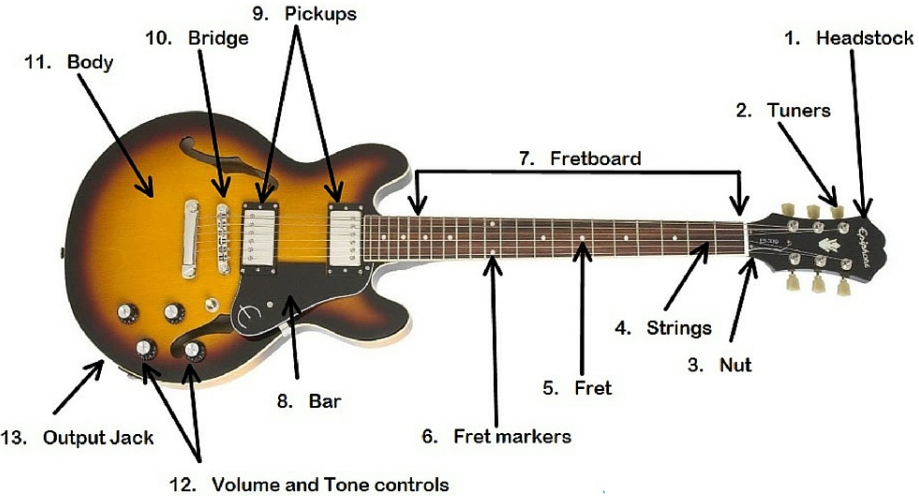
\includegraphics[width=0.9\textwidth]{guitar_parts.png}
		\caption{Illustration of an electric guitar and its parts \cite{coustii}.}
		\label{fig:guitar_parts}
\end{figure}
\todo[inline]{Sebastian: Maybe remove blue box?}

In the figure several parts are highlighted, but not all of them influence the sound, in the case where the guitar is not amplified. The pickups, the volume and the tone control have a large influence on the sound, when amplified, but they have no influence when not amplified. The Tuners do have an influence on the sound, but more in the sense of making sure the guitar is in tune, which also is more or less the case with the fretboard. 
The parameters that will be investigated and have an influence on the sound, when not amplified, are:

\begin{itemize}
 \item String thickness and material
 \item String action
 \item Bridges
\end{itemize}

\subsection{String thickness and material}
String thickness (gauge) affects the sound of a guitar a lot. String gauge affects the tone of the sound and the sustain of the sound. Tone is a very broad term, which says something about how a string sounds. Often tone is described in subjective terms such as warm, deep, crunchy etc \cite{premierguitar}. Sustain describes the period from when a tone is played until it fades out. Thicker strings will increase the sustain compared to thinner ones. Thicker strings will also increase the volume compared to thinner ones \cite{Helsinki}.
The material of the string also have an effect on its sound. Some of the materials used for electric guitar strings are: Nickel-plated steel, pure nickel and Stainless steel. Describing how the string material affects the sound is also often done in similar terms as for describing tone. E-Home Recording Studio fx. describes Nickel-plated steel as follows:
\\*
\\*
\textit{"Nickel-Plated Steel – which has a good combination of warmth and brightness, a strong picking attack, and is the most popular option."}\cite{E-Home}

\subsection{String action}
String action describes the distance from the strings to the fretboard on a guitar. A higher action allows the strings to vibrate more freely, and thereby increasing the sustain of the tone \cite{sweetwater}. If the string action is set too low, distortion can occur when a note is tapped.  

\subsection{Bridges}
The bridge on an electric guitar is where the playable area of the guitar strings begin. The purpose of the bridge is to keep the strings fixed on the body, but without adding too much friction to the strings. This is because it is wanted to transfer as less string vibration to the bridge as possible. Two main categories of electrical guitar bridges exist: the fixed bridges and the moving bridges. The type of bridge has an effect on several aspects when playing the guitar, but it is the string-friction on the bridge that has the largest effect on the sound \cite{seymourduncan}.
\\*
\\*
Other physical parts on an electric guitar such as the fretboard, the nut and the body does have an effect on the not amplified sound, because some of the string vibration will be transferred to these parts. These parts are however parts that are difficult to change, without decreasing the quality set by the factory.   


\todo[inline] {Sebastian: We need to explain the difference between the two volume control and tone control types}




 \section{Pickups on an electric guitar}
One of the most important parts of an electric guitar, is the transducer which converts the strings vibrations into an electrical signal. This is done with pickups, which as seen in \autoref{fig:guitar_parts}, is placed on the body. Typically an electric guitar has two or three pickups and the type and combination of pickups can vary. Two types of pickups are the single coil pickups and the dual coil (Humbucker) pickups. The electric equivalent to a single coil pickup is shown in \autoref{fig:electric_pickup}

\begin{figure}[h!]
\centering
\begin{circuitikz}\draw (0,0)
to[L=$L$]  (3,0)
to[R=$R$] (5,0)
(5,-1)to[short,-o](6,-1)
(5,0)to[short](5,-2)
to[C=$C$] (0,-2)
(0,-1)to[short,-o](-1,-1)
(0,-2)to[short] (0,0)
%to[short] (0,0)
;\end{circuitikz}
\caption{Electric equivalent of a single coil pickup \citep{build_your_guitar}.}
\label{fig:electric_pickup}
\end{figure}

A single coil pickup can be described as a an ideal inductor and a resistor in series, in parallel with a capacitor. This circuit is for the case when the guitars strings doesn't vibrate. When one or more strings are played, the circuit is expanded as shown in \autoref{fig:electric_pickup_strings}.

\begin{figure}[h!]
\centering
\begin{circuitikz}\draw (0,0)
to[L=$L$]  (3,0)
to[R=$R$] (5,0)
to[short, -o](6,0)
(5,0)to[C=$C$] (5,-2)
(6,-2)to[short, o-] (0,-2)
to[sV=$String$] (0,0)
%to[short] (0,0)
;\end{circuitikz}
\caption{Electric equivalent of a single coil pickup, when strings are played \citep{build_your_guitar}.}
\label{fig:electric_pickup_strings}
\end{figure}

When the strings are vibrates, they act as an \gls{ac} supply. The output signal from the pickup is then the voltage over the capacitor  \citep{build_your_guitar}. 
The complete circuit in an electric guitar is a bit more complicated, since an electric guitar often contains a volume control, one or more tone controls etc. A simple circuit of an electric guitar with one volume control and one tone control, is shown in \autoref{}

\begin{figure}[h!]
\centering
\begin{circuitikz}\draw (0,0)
to[L=$Pickup$]  (0,4)
to[short] (2,4)
to[vR=$Tone$ $pot$] (2,2)
to[C=$Tone$ $C$] (2,0)
to[short](0,0)
(2,4) to[short](5,4)
to[pR=$ $](5,0)
to[short](2,0)node[ground]{}
%Jack
(5.3,2)to[short]node[left,above]{$Volume$ $pot$}(6.6,2)
to[short](6.9,1.7)
to[short](7.2,2)
(7.5,2)to[short](7.5,1)
to[short](6,1)
to[short](6,0)
to[short](5,0)
(7.5,2)to[short](7.7,2)
to[short]node[right]{$Jack$ $input$}(7.7,1)
to[short](7.5,1)
%end Jack
;\end{circuitikz}
\caption{Simple circuit of an electric guitar with one volume control and one tone control \citep{electricalfun}.}
\label{fig:simple_guitar_circuit}
\end{figure}

The tone control is a simple lowpass filter and the volume control is a potentiometer. 

\subsection{Output impedance of an electric guitar}
A test was made to find the output impedance of an electric guitar. The test was made on a Fender Squier Classic Vibe Telecaster, and was tested with three pickup settings. The complete test journal can be seen in \autoref{app:output_impedance}. In \autoref{tab:impedance_test} the results from the output impedance test on the guitar is shown.

\begin{longtable}[h!]{ |m{\dimexpr 0.34\linewidth-2\tabcolsep}| 
          m{\dimexpr 0.33\linewidth-2\tabcolsep}| 
          m{\dimexpr 0.33\linewidth-2\tabcolsep}|   } 
\caption{Results from output impedance test of an electric guitar.} \label{tab:impedance_test} \\ 
 
\hline 
%%%%%%%%  
\textbf{Pickup setting} & \textbf{Minimum output impedance} & \textbf{Maximum output impedance} \\ 
%%%%%%%% 
\hline 
\endfirsthead     
\multicolumn{3}{c}{{{\footnotesize \bfseries \tablename\ \thetable{} -- Continued from previous page.}}} \\  
\hline 
%%%%%%%%  
\textbf{Pickup setting} & \textbf{Minimum output impedance} & \textbf{Maximum output impedance} \\ 
%%%%%%%%  
\hline 
\endhead       
\hline \multicolumn{3}{|r|}{{Continues on next page.}} \\ \hline 
\endfoot     
\hline 
\endlastfoot 
%%%%%%%% Content of table 
Neck & \SI{6220}{\ohm} at \SI{10}{\hertz} & \SI{58,51}{\kilo\ohm} at \SI{5167}{\hertz} \\ \hline
Bridge & \SI{7863}{\ohm} at \SI{10}{\hertz}  & \SI{73.06}{\kilo\ohm} at \SI{4010}{\hertz}\\ \hline
Neck and bridge & \SI{3563}{\ohm} at \SI{10}{\hertz} & \SI{53.43}{\kilo\ohm} at \SI{5702}{\hertz}\\ \hline
\end{longtable}

\subsection{Frequency area of an electric guitar}
A test was made to see which frequencies can be played on an electric guitar. The test was made with a Fender Squier Classic Vibe Telecaster, and was tested with two pickup settings. The complete test journal can be seen in \autoref{app:frequency_area}. In \autoref{tab:impedance_test} the results from the frequency spectrum test on the guitar is shown.

\begin{longtable}[h!]{ |m{\dimexpr 0.34\linewidth-2\tabcolsep}| 
          m{\dimexpr 0.33\linewidth-2\tabcolsep}| 
          m{\dimexpr 0.33\linewidth-2\tabcolsep}|   } 
\caption{Results from output impedance test of an electric guitar.} \label{tab:impedance_test} \\ 
 
\hline 
%%%%%%%%  
\textbf{Pickup setting} & \textbf{Lowest significant frequency} & \textbf{Highest significant frequency} \\ 
%%%%%%%% 
\hline 
\endfirsthead     
\multicolumn{3}{c}{{{\footnotesize \bfseries \tablename\ \thetable{} -- Continued from previous page.}}} \\  
\hline 
%%%%%%%%  
\textbf{Pickup setting} & \textbf{Lowest significant frequency} & \textbf{Highest significant frequency} \\ 
%%%%%%%%  
\hline 
\endhead       
\hline \multicolumn{3}{|r|}{{Continues on next page.}} \\ \hline 
\endfoot     
\hline 
\endlastfoot 
%%%%%%%% Content of table 
Neck & Around \SI{80}{\hertz} & Around \SI{4400}{\hertz} \\ \hline
Bridge & Around \SI{80}{\hertz}  & Around \SI{4400}{\hertz}\\ \hline
\end{longtable}




\section{Effect on an electric guitar}

Electrical guitars can have more effects than the ones that can be done with the physical part. Those additional ones will be described in the following part. The ones that are going to be described are:

\begin{itemize}
 \item Equalizing
 \item Reverberation
 \item Overdrive
 \item Distortion
 \item Chorus
 \item Flanger
 \item Wah-Wah
\end{itemize}


\newpage

\input{chapters/analysing/equalizing}\label{sec:equalizing} 
\subsection{Delay}
Delay is an audio effect which memorizes the input signal for a customized time, and then release it without changing anything else than the amplitude. The delayed signal can either be played back multiple times or only once . When the signal is delayed and then played back multiple times, it can either be amplified or attenuated. If the delayed signal is amplified, it will start to oscillate. If the wanted effect is an echo, the delayed signal shouldn't be kept alive, then the gain in the feedback must be reduced in order to attenuate the signal.  \autoref{fig:delay_block} shows a block diagram of a simple delay, "echo" unit.


\begin{figure} [htbp]
 \centering
\begin{picture}(0,0)%
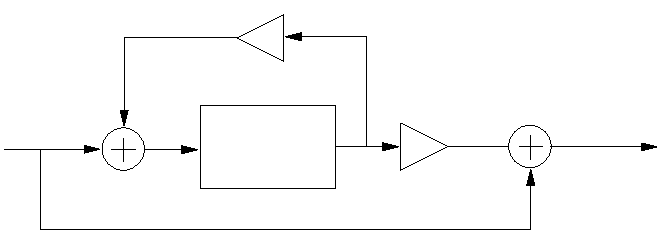
\includegraphics{delay.pdf}%
\end{picture}%
\setlength{\unitlength}{4144sp}%
%
\begingroup\makeatletter\ifx\SetFigFont\undefined%
\gdef\SetFigFont#1#2#3#4#5{%
	\reset@font\fontsize{#1}{#2pt}%
	\fontfamily{#3}\fontseries{#4}\fontshape{#5}%
	\selectfont}%
\fi\endgroup%
\begin{picture}(5035,1329)(1491,-118)
\put(4726,704){$Gain$}%

\put(3106,479){$Delay$}%

\put(5814,672){$Output$}%

\put(1506,659){$Input$}%

\end{picture}%

  \caption{The photo shows a block diagram on a delay unit \citep{delay_block}}
  \label{fig:delay_block}
\end{figure}

The block diagram \autoref{fig:delay_block} shows a delay unit with a feedback line that has an adjustable gain. The feedback signal is either attenuated or amplified depending on the gain value and then added to the delay line input \cite{delay_echo}. The following \autoref{fig:delay_echo} shows the effect in time domain.

\begin{figure} [htbp]
 \centering
  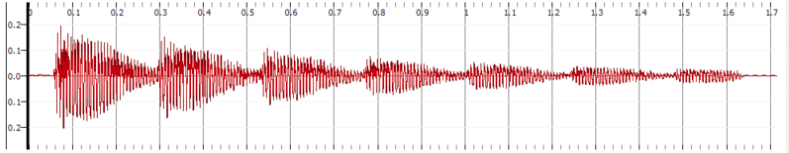
\includegraphics[width=1\textwidth]{delay_echo}
  \caption{The photo shows a echo in time domain}
  \label{fig:delay_echo}
\end{figure}
\todo[inline]{make figure i matlab}

The \autoref{fig:delay_echo} shows that the main signal is repeated and attenuated 6 time before it is totally attenuated. A time domain diagram is shown at \autoref{fig:delay_timed}.

\begin{figure} [htbp]
 \centering
\begin{picture}(0,0)%
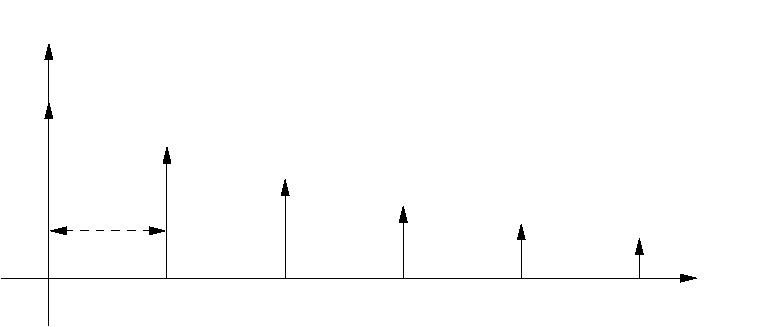
\includegraphics{delay_timed.pdf}%
\end{picture}%
\setlength{\unitlength}{4144sp}%
%
\begingroup\makeatletter\ifx\SetFigFont\undefined%
\gdef\SetFigFont#1#2#3#4#5{%
  \reset@font\fontsize{#1}{#2pt}%
  \fontfamily{#3}\fontseries{#4}\fontshape{#5}%
  \selectfont}%
\fi\endgroup%
\begin{picture}(5843,2478)(4129,-5833)
\put(9496,-5506){$Time$}%
\put(4231,-3526){$Magnitude$}%
\put(4591,-4291){$Main$}%
\put(5536,-4606){$G$}%
\put(6436,-4876){$G^2$}%
\put(7336,-5056){$G^3$}%
\put(8236,-5191){$G^4$}%
\put(9136,-5281){$G^5$}%
\put(4861,-5056){$t\Delta$}%
\put(6256,-5776){$t2$}%
\put(5356,-5776){$t1$}%
\put(7156,-5776){$t4$}%
\put(8056,-5776){$t5$}%
\put(8956,-5776){$t6$}%
\end{picture}%
  \caption{The figure shows the impulse respond of the delay unit}
  \label{fig:delay_timed}
\end{figure}
\label{sec:delay} 
\section{Reverberation}
Reverberation is \label{sec:reverberation} 
\subsection{Overdrive and Distortion} 

The distortion effects changes the sound of the played instrument by increasing the gain. It is commonly used the with the electric guitar. The sound changes due to the clipping effect. \\
\todo[inline]{Muhammed: "It is commonly used in the with the electric guitar" does something missing?}

The clipping effect is a way of changing the waveform when an amplifier is over driven; forcing it to deliver an output that is higher than its maximum capability. \\
The part of the waveform where the amplifier is asked to get a value higher than its maximum capacity gets the maximum value the amplifier can give. It means that all the parts of the waveform where the amplifier is pushed more than its capacity will have the same amplitude. The signal is then 'clipped'. An illustration of this effect is shown in \autoref{fig:clipping1}.\\

\begin{figure} [htbp]
	\centering
  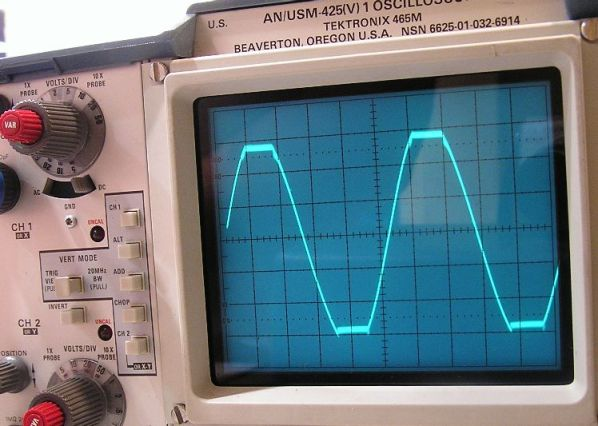
\includegraphics[width=0.7\textwidth]{clippingeffect.jpg}
  \caption{Photo showing the effect of clipping, a consequence of the overdrive or distortion effect.}
  \label{fig:clipping1}
\end{figure}


The consequences in the frequency domain are that the clipping effect creates more harmonics at high frequency than the signal without the clipping effect. \\

The clipping effect in signal processing happens when the amplitude is limited by a number and if during the processing the amplitude surpasses this limit, clipping happens because the value is then maxed to the maximum number that can be handled digitally. The maximum amplitude that can be handled is determined by the number of bits the system uses. The maximum number for a \SI{16}{\bit}  signed integers system is $\frac{2^{16}}{2} = \SI{32768}{\cdot}$ which means that if a value has an amplitude higher than this number the clipping effect occurs. \\

In any clipping technique, there is a creation of new harmonics. In the case of soft clipping, the new harmonics are multiples of the harmonics of the original tone. Valve Overdrive is a soft clipping technique for instance. In the case of hard clipping, they are not multiples which results to what is called intermodulation. Hard clipping usually happens when the harmonics of the original signal are not related by a multiple. Transistor overdrive is an example of hard clipping.  Effects of hard and soft clipping on the waveforms are shown in \autoref{fig:clipping2}.

In the previous paragraphs, distortion and overdrive has been explained as if they are the same effects. In fact, there is a small difference between the two. Distortion changes the original tone more than overdrive which means that distortion will generate more extra harmonics than overdrive and their amplitude tend to be higher. Overdrive effect has "cleaner" consequences on the final tone than distortion. Overdrive is often assigned to soft clipping while distortion is assigned to hard clipping.

\begin{figure} [htbp]
	\centering
  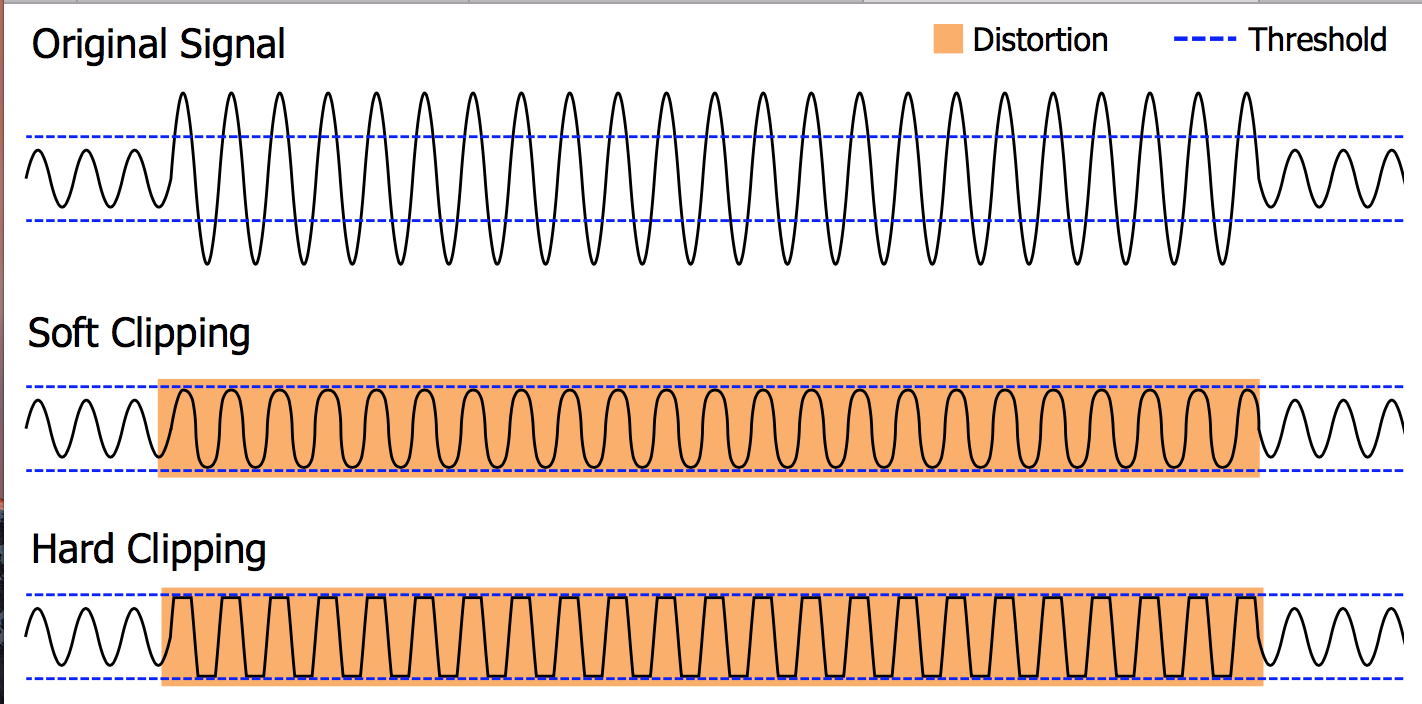
\includegraphics[width=0.7\textwidth]{softhardclipping.png}
  \caption{Photo showing the effect of hard and soft clipping, a consequence of the overdrive or distortion effect.}
  \label{fig:clipping2}
\end{figure}


\label{sec:overdrive} 
\subsection{Chorus and Flanger Effect} \label{sec:chorus} 

%\label{chor_flang}

The chorus effect is obtained when a signal is delayed and then mixed with its original version \citep{chorus_gibson} \citep{chorus_apple}. \\
The chorus effect takes a single audio signal as input and applies different delay values to it. Chorus effect using one delay is called flanger. Each of the delayed signals are then mixed with the original audio input. \\
A \gls{lfo} can be used to make the delay times vary. Different \gls{lfo}s can be used for each of the delay channels to make a richer sound mix and avoiding repetitive sound but it implies more computations. The same \gls{lfo} can be used for all the delay channels but not at the same cycle for each delay \citep{chorus_testtone}. \\ 

Different parameters on the chorus effect can changed by settings on the hardware. Some of these are:\\
\begin{itemize}
\item \textbf{Delay time}: The time difference between the original sound and the delayed one (The frequency of the signal from the \gls{lfo}).
\item \textbf{Chorus size}: The number of delayed sounds that will be mixed.
\item \textbf{Depth}: The amplitude of the signal from the \gls{lfo}.
\item \textbf{Waveform}: The waveform of the signal from the \gls{lfo} can be changed to triangle, sine, log ect. \citep{hobby_hour_chorus}
\item \textbf{Gain}: The amplification of the delayed signal.
\end{itemize} \citep{chorus_parameters}

A block diagram for  the chorus and flanger effect is shown in \autoref{fig:chorus_diag}.

\begin{figure} [htbp!]
	\centering
\begin{picture}(0,0)%
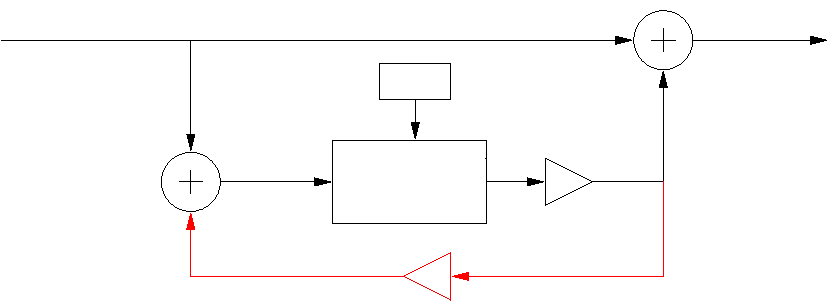
\includegraphics{chorus_diag.pdf}%
\end{picture}%
\setlength{\unitlength}{4144sp}%
%
\begingroup\makeatletter\ifx\SetFigFont\undefined%
\gdef\SetFigFont#1#2#3#4#5{%
	\reset@font\fontsize{#1}{#2pt}%
	\fontfamily{#3}\fontseries{#4}\fontshape{#5}%
	\selectfont}%
\fi\endgroup%
\begin{picture}(6327,3018)(3766,-3493)
\put(6706,-1366){\color[rgb]{0,0,0}LFO}%

\put(8101,-1636){\color[rgb]{0,0,0}Gain}%

\put(3781,-646){\color[rgb]{0,0,0}Input}%

\put(9406,-646){\color[rgb]{0,0,0}Output}%

\put(6571,-1906){\color[rgb]{0,0,0}Delay}%

\put(6616,-3211){\color[rgb]{1,0,0}Delay}%

\put(8101,-2986){\color[rgb]{1,0,0}Gain}%

\put(6706,-2671){\color[rgb]{1,0,0}LFO}%

\end{picture}%



\caption{Block Diagram of the chorus effect.}
\label{fig:chorus_diag}
\end{figure}


As it can be seen on the block diagram in figure \autoref{fig:chorus_diag}, a signal that hasn't been affected by any changes is added to the same signal delayed, controlled by the \gls{lfo}. The addition is done just before the output. The chorus effect is represented by the black and the red parts of the block diagram. The flanger effect is represented only by the black parts of the block diagram. In \autoref{fig:chorus_and_flanger_time} the impulse response of the chorus and the flanger effect are shown. Its is seen that with a pulse as the input, in the flanger effect, the output will be the original pulse, followed by an echo. The period before this echo arrives varies, based on the \gls{lfo}. When using the chorus effect several echoes will arrive, still with varying delay time. 

\begin{figure}[htbp!]
\centering
\def\svgwidth{\columnwidth}
\scalebox{0.8}{\input{figures/analysing/chorus_and_flanger_time_domain.pdf_tex}}
\caption{Impulse response of the flanger effect (black) and the chorus effect (red).}
		\label{fig:chorus_and_flanger_time}
\end{figure}










\label{sec:chorus} 
\subsection{Wah-Wah}\label{sec:wah-wah} 

The effect takes the original signal and mix it with another signal that passes through a bandpass filter. The bandpass filter is time varying, which means that it changes its position in the frequency spectrum \citep{wah-wah_course}. \\
The automatic Wah-Wah effect have some different parameters that can be changed to customize the effect:\\

\begin{itemize}
	\item \textbf{The \gls{lfo} frequency}: it sets the speed at which the bandpass filter moves in the frequency spectrum.
	\item \textbf{\gls{lfo} start phase}: Determine where should the bandpass filter start.
	\item \textbf{\gls{lfo} depth}: the range of frequencies it should work on, high depth gives a bigger range and vice versa.
\end{itemize} \citep{wah-wah_audacity}

A block diagram of the effect is illustrated in \autoref{fig:wah_diag}.  

\begin{figure} [htbp]
	\centering
\begin{picture}(0,0)%
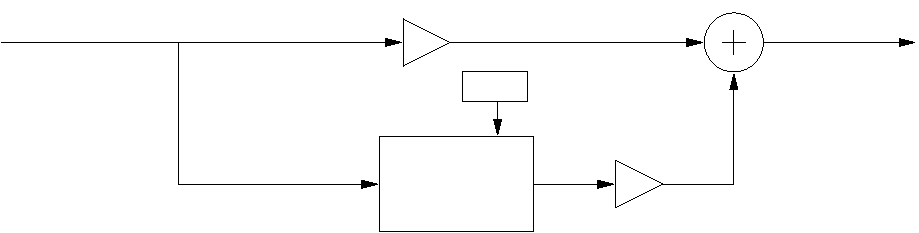
\includegraphics{wah_diag.pdf}%
\end{picture}%
\setlength{\unitlength}{4144sp}%
%
\begingroup\makeatletter\ifx\SetFigFont\undefined%
\gdef\SetFigFont#1#2#3#4#5{%
  \reset@font\fontsize{#1}{#2pt}%
  \fontfamily{#3}\fontseries{#4}\fontshape{#5}%
  \selectfont}%
\fi\endgroup%
\begin{picture}(6999,1770)(2689,-2233)
\put(6841,-1591){\textit{Wah-Wah Gain}}%
\put(5626,-2041){$Filter$}%
\put(6136,-1186){\textit{LFO or Pedal}}%
\put(2746,-646){$Input$}%
\put(8686,-646){$Output$}%
\put(5626,-1816){$Bandpass-$}%
\put(5986,-646){$Gain$}%
\end{picture}%
	\caption{Block diagram of the wah-wah effect}
	\label{fig:wah_diag}
\end{figure}

It can be seen on the block diagram that the filtered signal is added to the direct signal. Thus, this block diagram is a representation of the wah-wah effect.  \\


The phaser effect can be created by using a band-stop filter instead of a bandpass filter using the same block diagram presented in \autoref{fig:wah_diag} \citep{wah-wah_cardiff}. \\

There is another type of wah-wah effect called M-fold wah-wah which uses multiple M-tap bandpass filters that move around the spectrum at the same time \citep{wah-wah_cardiff}. \\

An example of a time domain response is shown in figure \autoref{fig:wah-wah-response}. \\

\begin{figure} [htbp!]
	\centering
	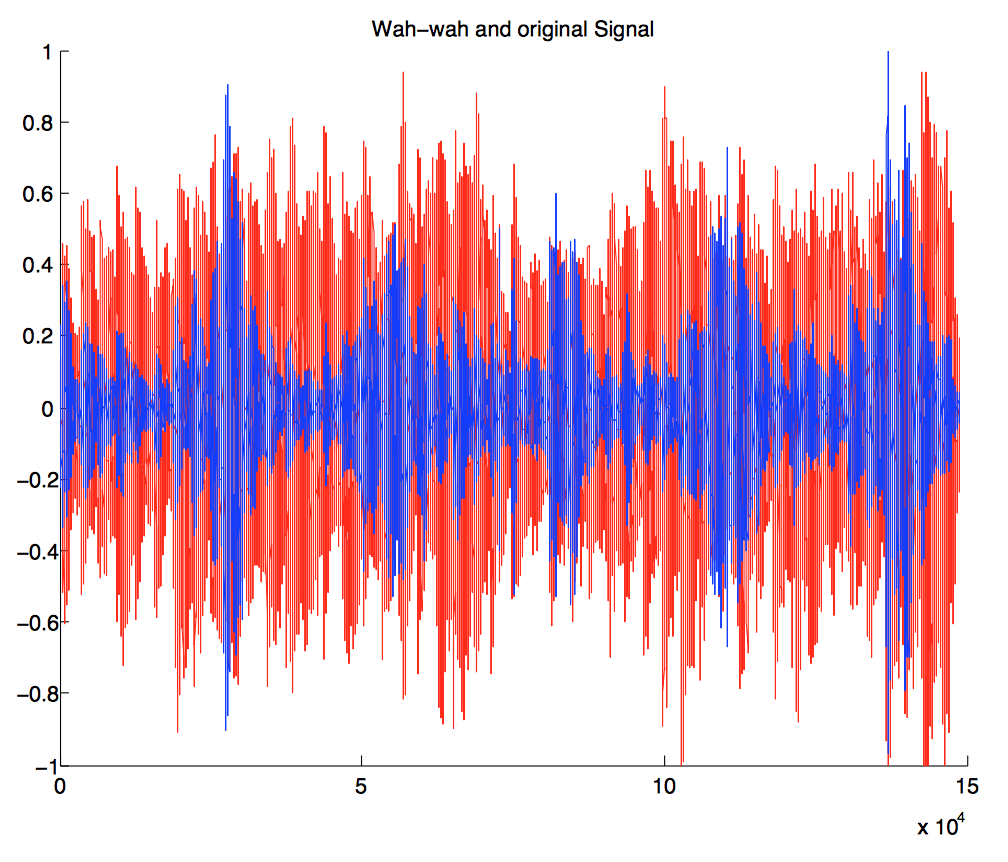
\includegraphics[width=0.6\textwidth]{wah-wah-response.png}
	\caption{Time domain response of the original sound (red) and the one after having the wah-wah effect (blue) \citep{wah-wah_cardiff}.}
	\label{fig:wah-wah-response}
\end{figure}
\todo[inline]{write about wah wah frequency in text}

\todo[inline]{Jonas: Muhammed, can you explain the above time domain spectra?(and the block diagram)}
\todo[inline]{Sebastian: Maybe make figure our self, because axis descriptions are missing now}

As it can be seen on \autoref{fig:wah-wah-response}, the wah-wah effect reduced the amplitudes of many parts of the wave-form compared to the signal without the wah-wah effect. Some of the them remained the same. It is due to the bandpass-filtering.
In \autoref{fig:wah_wah_frequency} an illustration of the bandpass filter in the wah-wah effect in frequency domain is shown. 

\begin{figure}
\centering
\def\svgwidth{\columnwidth}
\input{figures/analysing/wah_wah_frequency_domain.pdf_tex}
\caption{Frequency domain illustration of bandpass filter in the wah-wah effect}
		\label{fig:wah_wah_frequency}
\end{figure}

It is shown that the bandpass filter can be moved in frequency. This movement is done either by an \gls{lfo} or with an expression pedal.
\label{sec:wah-wah} 

\section{Platform comparing}
In order to implement the previous discussed effects digitally, a platform has to be chosen. In this section a list of possible platforms for the effect implementation will be analysed. The following platforms will be analysed:

\begin{itemize}
\item Rasperry pi
\item \gls{dsp}
\item \gls{fpga}
\end{itemize}

\subsection{Raspberry pi}
There exist different generations of the Raspberry pi, but the one that will be analysed is the Raspberry pi 3 model B, since it is the latest version. 
A Raspberry pi is a \gls{sbc} at the size of a credit-card. A picture of the Raspberry pi 3 model B, is shown in \autoref{fig:RP3mB}.

\begin{figure}[h]
	\centering
		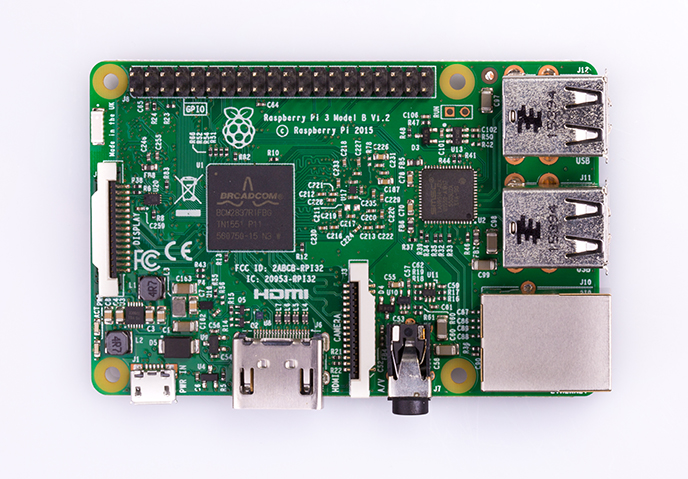
\includegraphics[width=0.7\textwidth]{Raspberry_pi_3_model_B.jpg}
		\caption{Picture of the Raspberry Pi 3 model B \cite{Raspberry_pi}.}
		\label{fig:RP3mB}
\end{figure}

The Raspberry pi 3 model B has a 1.2 GHz Quad-core ARM processor, supports wireless LAN and Bluetooth 4.1. It has 1GB RAM and has connectors for micro SD cards \cite{Raspberry_pi}.
The Raspberry Pi is Linux based, but can also run Windows \cite{sparkfun_Raspberry_pi}. This makes the Raspberry pi 3 model B suited for a wide range of projects. This is both its advantage and its disadvantage if a specialized platform is wanted. 

\subsection{Digital Signal Processor}
A \gls{dsp} is a processor, which is optimized for high-speed numerical operations such as: Addition, subtraction and multiplication. A typical \gls{dsp} system includes an anti-aliasing filter, an \gls{adc}, a \gls{dsp}, a host interface, a \gls{dac} and a anti-imaging filter. A block diagram of the typical \gls{dsp} system is shown in \autoref{fig:typ_dsp}.

\begin{figure}
\centering
\def\svgwidth{\columnwidth}
\input{figures/analysing/DSP_typical.pdf_tex}
\caption{Block diagram of a typical \gls{dsp} \cite{AnalogDialogue}.}
		\label{fig:typ_dsp}
\end{figure}

These high-speed numerical operations make the \gls{dsp} suited for real-time applications, and a \gls{dsp} can work both as a sample-based system and as a frame-based system. 
Two terms are commonly used for describing the processing power of a \gls{dsp}. These are \gls{mips} and \gls{mops}. The requirements of the \gls{dsp} can be found, based on the sampling interval and the number of operations needed between each sample. This is shown in \eqref{eq:MOPS}.

\begin{equation}\label{eq:MOPS}
        DSP_{speed} = \frac{Operations}{T_s}\addunit{MOPS}
    \end{equation}

    \startexplain
        \explain{$DSP_{speed}$ is the \gls{dsp}'s processing power}{MOPS}
        \explain{$Operations$  is the number of operations}{1}
        \explain{$T_s$ is the sampling interval}{\si{\second}}
    \stopexplain


\gls{mips} and \gls{mops} are not the same, but related in the way that each \gls{dsp} instruction containe a numbers for operation  \cite{AnalogDialogue}. E.g. a \gls{dsp} with 4 \gls{mips} and 8 \gls{mops} means that the \gls{dsp} can preform 2 operation for each instruction.


\label{sec:platform_comparing}
\subsection{FPGA}


The FPGA (Field Programmable Gate Array) is a circuit that contains multiple logic blocks and routing channels.\\
The hardware configuration is customizable in order to meet the user’s demands in the digital domain; unlike ICs where the connections between the transistors cannot be changed, it is possible to make a custom architecture on an FPGA. \\
As said, the FPGA consists of multiple logic blocks often called logic cells. Each cells consists of an LUT (Look-up table) and a flip-flop. The LUT has four inputs and the flip-flop one clock input. The LUT contains a small Random Access Memory and performs logical operation. \\
Around the logic blocks, there are multiple I/O blocks which can also be programmed to an output or input for instance.  \\
An FPGA contains a configuration logic that is connected to the flash memory which contains information about the connection between the logic blocks and the architecture inside the block itself. The more logic blocks are used and programmed, the bigger the flash memory storage size has to be. An overview of the structure of the FPGA is shown in \autoref{fig:fpgastructure} and the structure of the logic block in \autoref{fig:logicblockstruct}. \\
\newline

\begin{figure}[htbp]
	\centering
	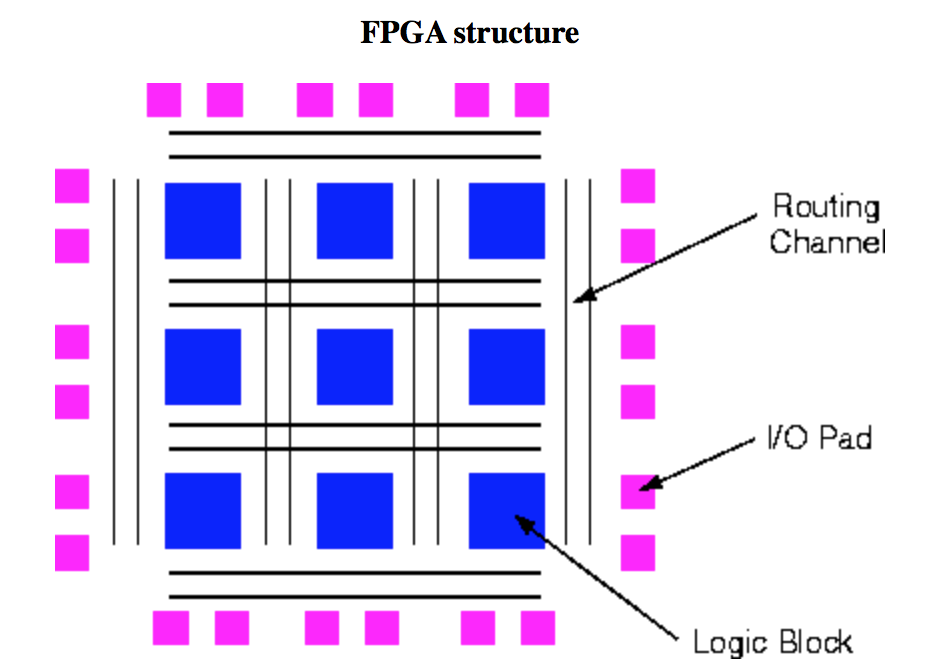
\includegraphics[width=0.7\textwidth]{fpgastructure}
	\caption{Scheme of FPGA components.}
	\label{fig:fpgastructure}
\end{figure}

\begin{figure}[htbp]
	\centering
	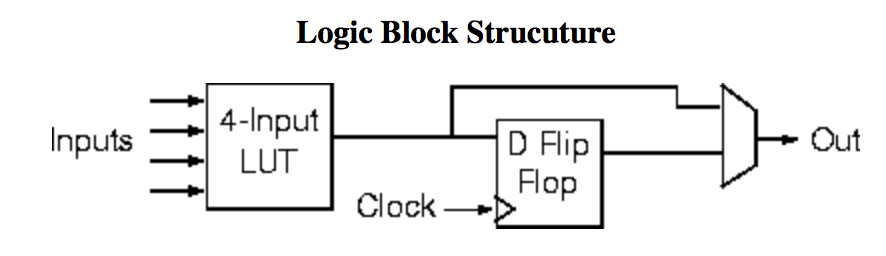
\includegraphics[width=0.7\textwidth]{logicblockstruct}
	\caption{Structure of a logic block.}
	\label{fig:logicblockstruct}
\end{figure}


The biggest advantage of the FPGA is to make multiple processes at the same time by isolating some logic blocks and I/Os for a specific task, which is not possible with ICs. A micro controller needs to run tasks in sequence, one after the other. If different tasks needs to be done in a restricted timing, this parameter can be crucial. 
By using parallelism and having fast I/Os, the FPGA can be very powerful. \\

The FPGA can be programmed using a hardware description language like VHDL or Verilog. \\

FPGA are certainly more efficient than ICs and normal micro controller but they are also more expensive especially if it’s about cloning a pre-existing micro controller without any personal added value. They are also power demanding. The FPGA has a configuration flash memory which means that there is no need for the user to intervene after a reboot, but at each boot the FPGA is programmed from scratch using the data from the flash memory which can drastically increase the boot time as well as the power consumption. It is more complicated to program an FPGA than using an IC or micro controller because it has to be designed by the user. \\








 \label{sec:FPGA}
\section{The benefits of using digital signal processing over analog}
\subsection{Quality}

The bandwidth in an analog sound signal can be increased infinitely unlike the digital one where it is limited by the sampling rate that is being used. \\

The quality in the digital signal is  lower because in the digital domain there is what is called the digital noise. It occurs after sampling, and increase when the sound between samples get less and less smooth. On the other side, in the analog domain, the signal is not sampled, it is the real one so this problem do not exist. Errors can also occur due to bit depth, bit depth limits the values that the sample can take, which means that even with high sample rate but low bit depth, the digital track can sound different. The number of values that can be sampled is defined by the number of bits per sample, and the number of values are then $2^{number of bits}$ \citep{analog_quality}.\\
It can then be inferred that there are quantization noise and errors in digital signals, which do not exist in analog signals. The same goes for aliasing \citep{analog_aliasing}. 

\subsection{Mobility}

Digital Sounds are more portable than analog ones, they can be played on different machines and copied without losing any information unlike the analog sound that can only be played on a tape for instance \citep{analog_quality}. 

\subsection{Lifetime}

A digital sound can last longer than an analog one. A Vinyl disk for example can get damaged and impact the sound stored on it and thus the quality. On the other side, a digital file saved on a computer cannot get damaged physically, unless the storage does, and can be duplicated very easily to preserve it. With the rise of cloud systems, the loss of a digital file is nearly impossible unless intentional \citep{analog_storage}.


\subsection{Requirements}

It is easier to fulfil given requirements using digital over analog signal processing because the user has more control over the digital controller than the analog one. If at anytime, the engineer realizes that the components needs more processing power, it can be easily upgraded \citep{analog_requirements}.

\subsection{Functionality and Customization}

With only one \gls{dsp}, it is possible to program numerous effects, personalize them and even create custom ones. Effects presented in \autoref{sec:effects} are just part of a growing and endless world of digital effects. 

  \label{sec:digital_vs_analog}
\chapter{Problem Analysis Conclusion}\label{ch:analysing_cl}
In the previous \autoref{ch:analysing}, different sound personalizations that can be done without any effect pedals on an electric guitar has been scrutinized. Then, different effects in the digital domain has been presented followed by the advantages of digital signal processing over analog. Different devices for \gls{dsp} have also been presented.  \\
\newline
It can be inferred from the analysis \autoref{sec:electric_guitar_theory} that the level of customization when using the physical part of the guitar is very low. However, there is a great number of effects that can be attached to this type of guitars and give the musician more possibilities, some of them presented in \autoref{sec:effects}.  \\
During the last decades, a lot of improvements have been made in the digital domain. The digital sound quality is now comparable to the analog one even for an audiophile. The advantages of using analog signal processing over digital are getting weaker. On the other side, various reasons can push the user to choose digital over analog: portability, lifetime, personalization, ease of use...

\chapter{Problem statement}
Based on the knowledge found in the analysis, and the conclusions drawn from it, a problem statement can be made. The following problem statement will be the focus of the rest of the project:
\\
\\
\textbf{How can a number of digital guitar effects be designed and implemented using Digital Signal Processing?}
\section{Delimitations}
The following delimitations are made for the rest of the project:

\begin{itemize}
\item Since the main focus of this project will be to design and digitally implement guitar effects, the design of the analog parts of the project will, as often as possible, be done using \gls{ic}'s. 
\item It is chosen to work with mono audio, since this will be sufficient for the main focus of the project.
\end{itemize} 
 
\chapter{Product Requirements}
This chapter lists the requirements for the effects presented in the analysis. 

\begin{figure}[htbp]
	\centering
\begin{picture}(0,0)%
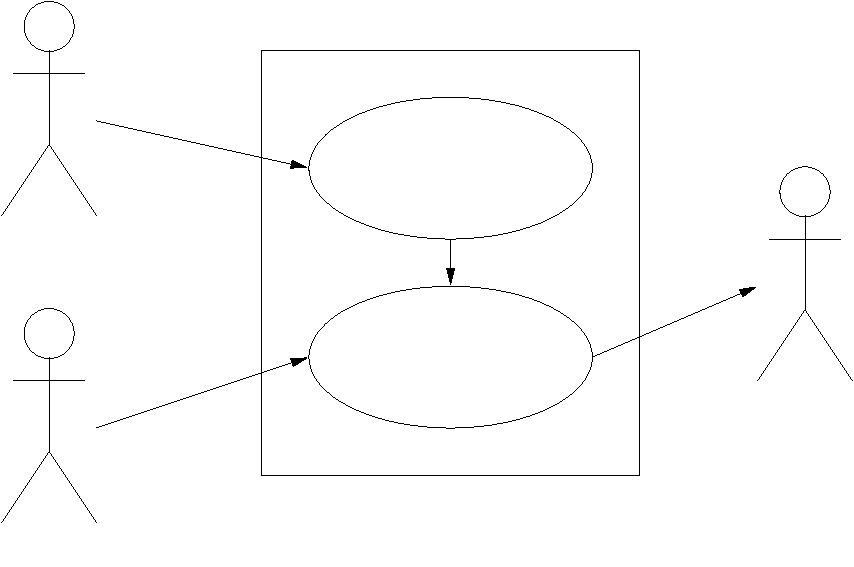
\includegraphics{Use_case.pdf}%
\end{picture}%
\setlength{\unitlength}{4144sp}%
%
\begingroup\makeatletter\ifx\SetFigFont\undefined%
\gdef\SetFigFont#1#2#3#4#5{%
  \reset@font\fontsize{#1}{#2pt}%
  \fontfamily{#3}\fontseries{#4}\fontshape{#5}%
  \selectfont}%
\fi\endgroup%
\begin{picture}(6507,4318)(1426,-4900)
\put(1531,-2491){User}%
\put(4546,-3346){Effect}%
\put(4276,-1906){Effect select}%
\put(7111,-3751){Amplifier}%
\put(1441,-4831){Guitar}%
\end{picture}%
	\caption{A graphically overview of wanted functionality in form of an use case digram.}
	\label{fig:use_case}
\end{figure}

From \autoref{ch:analysing} some of the effect can be designed together, because the effect is using the same parts but multiply times or just a small difference. The following description tells shortly about the different in the effect block and which effect that can be designed together.

\paragraph{Basic filtering}
The only basis filter, which is explained in \autoref{ch:analysing} which is a basic filter without delay and time changing parameters is the Equalizer.


\paragraph{Time varying filter}
The only Time varying filter, which is explained in \autoref{ch:analysing} is the Wah-Wah.


\paragraph{Delay}
All the delay based effect have at lest one delay block and have both fast and slow delay. All the analysed delayed based effect in \autoref{ch:analysing} is:
\begin{itemize}
	\item Delay
	\item Flanger
	\item Chorus
	\item \gls{reverb}
\end{itemize} 

The block diagram in each effect shows that two and two effect have a common structure with using the same parts but multiply times. In another way the chorus is the flanger with 

\paragraph{Non-linear processing}
\begin{itemize}
	\item Distortion
	\item Overdrive
\end{itemize} 

\subsection{Block}

The requirements are divided into units, based on the effect analysis \autoref{ch:analysing}, since it is concluded in \autoref{ch:analysing} that only six general units need to be designed and all the presented effects can be created with those six. The unit that are going to be designed are the:



\begin{itemize}
	\item Bandpass filter
	\item Inverse bandpass filter
	\item Delay
	\item Gain
	\item Clipping
	\item \gls{lfo}
\end{itemize} 

 Besides the fact that each unit shall be designed individually, each unit interface should fit in the effect that is using it. Each unit has its own section where the requirements and their arguments are presented. To ensure that the units can fit and work together, basic requirements  are made on the processing component to be chosen afterwards first.
 
 
\newcommand{\reqbasis}{The delay unit must delay the input signal, in time defined by external unit.}

\reqPrefix{BS}
\section{Basis requirements}
Based on the \autoref{ch:analysing}, the delay requirement is as following

\begin{requirement}\label{req:dsp}
    \requirement{The processing component module are used to process the signal }
    \argument{It is concluded that the effect shall be made digitally}
\end{requirement}

\begin{requirement}\label{req:software}
    \requirement{Each unit must fit into a \gls{dsp} architecture}
    \argument{In order to be able to design all unit digitally}
\end{requirement}

\begin{requirement}\label{req:speed}
    \requirement{The calculation of one effect shall be faster than the sample frequency. }
    \argument{The processing component shall be fast enough to calculate at lest one effect between two sample}
\end{requirement}


\newcommand{\reqconverters}{The delay unit must delay the input signal, in time defined by external unit.}

\reqPrefix{Converter}
\section{Converters}
Based on \autoref{sec:pickups}, the requirements for the \gls{adc} and the \gls{dac} are as follows:

\begin{requirement}\label{req:ADC_resolution}
    \requirement{The \gls{adc} much have a resolution of at least 10 bits.}
    \argument{This requirement is made according to \autoref{eq:dB_max_min_guitar_out}.}
\end{requirement}


\begin{requirement}\label{req:ADC_Fs}
    \requirement{The sampling frequency of the \gls{adc} must be at least \SI{8.8}{\kilo \hertz}. }
    \argument{This requirement is made according to \autoref{tab:frequency_area}.}
\end{requirement}

\begin{requirement}\label{req:DAC_resolution}
    \requirement{The \gls{dac} much have a resolution of at least 10 bits.}
    \argument{This requirement is made according to \autoref{eq:dB_max_min_guitar_out}.}
\end{requirement}

\begin{requirement}\label{req:DAC_Fs}
    \requirement{The sampling frequency of the \gls{dac} must be at least \SI{8.8}{\kilo \hertz}. }
    \argument{This requirement is made according to \autoref{tab:frequency_area}.}
\end{requirement}
\newcommand{\reqbandpass}{The delay unit must delay the input signal, in time defined by external unit.}

\reqPrefix{BF}
\section{Bandpass filter (\reqPrefixName)}
Based on the \autoref{ch:analysing}, the delay requirement is as following

\begin{requirement}\label{req:bandpass_filter}
    \requirement{The bandpass filter unit must be able to increase the gain in its passband area}
    \argument{In order to be able to amplifier the the signal gain in specified frequencies}
\end{requirement}

\begin{requirement}\label{req:bandpass_filter1}
    \requirement{The center frequency must be able to change, defined by an external unit and internal preset}
    \argument{In order to be able to change the center frequency in Wah-Wah, and have preset center frequency in equalizer}
\end{requirement}

\begin{requirement}\label{req:bandpass_filter2}
    \requirement{The bandpass filter cross frequency at \SI{0}{\decibel} shall be at the previously and the next bandpass center frequency in any gain}
    \argument{In order to be able to make a flat frequency respond on the amplified frequency}
\end{requirement}
\newcommand{\reqInversebandpassfilter}{The delay unit must delay the input signal, in time defined by external unit.}

\reqPrefix{IBF}
\section{Inverse bandpass filter (\reqPrefixName)}
Based on the \autoref{ch:analysing}, the delay requirement is as following

\begin{requirement}\label{req:Inverse_bandpass_filter_ex}
    \requirement{The inverse bandpass filter unit must be able to attenuate the gain in its stopband area}
    \argument{In order to be able to attenuate the the signal gain in specified frequencies}
\end{requirement}

\begin{requirement}\label{req:Inverse_bandpass_filter_time}
    \requirement{The center frequency must be defined by internal preset}
    \argument{In order to attenuate the frequency with octave separation in the equalizer}
\end{requirement}

\begin{requirement}\label{req:nverse_bandpass_filter_center}
    \requirement{The bandstop filter cross frequency at \SI{0}{\decibel} shall be at the previously and the next bandstop center frequency}
    \argument{In order to be able to make a flat frequency respond on the attenuated frequency}
\end{requirement}

\newcommand{\reqdelay}{The delay unit must delay the input signal, in time defined by external unit.}

\reqPrefix{Delay}
\section{Delay}
Based on the \autoref{ch:analysing}, the delay unit requirements are as follows:

\begin{requirement}\label{req:delay_ex}
    \requirement{The unit must be able to delay a signal, with the delay time defined by an external unit.}
    \argument{In order to be able to control the delay time from an external unit.}
\end{requirement}

\begin{requirement}\label{req:delay_time}
    \requirement{The unit must be able to delay a signal, with a predefined delay time.}
    \argument{In order to be able to change the effect mode in the \gls{reverb} effect.}
\end{requirement}


\newcommand{\reqgain}{The delay unit must delay the input signal, in time defined by external unit.}

\reqPrefix{Gain}
\section{Gain}
Based on the \autoref{ch:analysing}, the delay requirement is as following

\begin{requirement}\label{req:gain_ex}
    \requirement{The delay unit must delay the input signal, in time defined by external unit.}
    \argument{In order to be able to change the delay time, the unit needs to depend on external unit}
\end{requirement}

\begin{requirement}\label{req:gain_time}
    \requirement{The delay unit must delay the input signal, in time defined by external unit.}
    \argument{In order to be able to change the delay time, the unit needs to depend on external unit}
\end{requirement}


\newcommand{\reqclipping}{The delay unit must delay the input signal, in time defined by external unit.}

\reqPrefix{Clipping}
\section{Clipping}
Based on \autoref{ch:analysing}, the clipping requirements are as follows:

\begin{requirement}\label{req:hard_clipping}
    \requirement{The clipping unit must be able to make hard clipping.}
    \argument{In order to be able to perform the distortion effect.}
\end{requirement}

\begin{requirement}\label{req:soft_clipping}
    \requirement{The clipping unit must be able to make soft clipping.}
    \argument{In order to be able to perform overdrive effect.}
\end{requirement}


\newcommand{\reqlfo}{The delay unit must delay the input signal, in time defined by external unit.}

\reqPrefix{LFO}
\section{Low frequency oscillator}
Based on \autoref{ch:analysing}, the \gls{lfo} requirements are as follows:

\begin{requirement}\label{req:lfo_ex}
    \requirement{The \gls{lfo} unit must have a frequency from \SI{0.1}{\hertz} to \SI{10}{\hertz}  }
    \argument{In order to be able to make a signal which is under the audibility range. }
\end{requirement}

\begin{requirement}\label{req:lfo_time}
    \requirement{The \gls{lfo} unit shall be able to make sinus, triangle, squared and sawtooth waveforms.}
    \argument{In order to create different effects like chorus, flanger and wah-wah.}
\end{requirement}


%%
\part{Design \& Construction}\label{pt:design} 
\graphicspath{{figures/design/}}
\chapter{Component choices}
\section{Digital Signal Processor Choice}

The chosen component is the \gls{dsp} for numerous reasons that are going to be presented in the following subsections.

\subsection{Advantage of the \gls{dsp} over the FPGA}

Some of the  reasons of choosing a \gls{dsp} over an FPGA in this project are:
 
\begin{itemize}

\item  The simplicity of designing with a \gls{dsp} due to the availability of all the simple functionalities in a micro-controller \citep{eetimes}. 

\item A \gls{dsp} is designed to perform signal processing task unlike the FPGA which purpose of creation was not related to signal processing but to program circuits \citep{eetimes}. 

\item A \gls{dsp} is more suitable in terms of cost/performance for \gls{mmac} per second lower than 3000, which means that it is better for low demanding applications \citep{eetimes}. 

\item FPGAs lack integrated DAC and ADC \citep{eetimes}. 

\item The \gls{dsp}s are more power efficient than the FPGAs which can be important if the effect is to be used on the move on battery power \citep{rtcmag}. 

\item A \gls{dsp} can be optimal if there are many operations that are repeated \citep{eetimes} \citep{hunteng}. 

\end{itemize}

\subsection{Advantage of the \gls{dsp} over the Raspberry Pi}

Some of the  reasons of choosing a \gls{dsp} over an Raspberry Pi in this project are:
 
\begin{itemize}

\item \gls{dsp}s are much faster for integer and floating mathematical calculations. A \gls{dsp} is designed to compute large and complex operations that are repetitive which makes it more suitable for this project \citep{diffbet} \citep{esp_simone}.   

\item A micro-controller, such as a Raspberry Pi, has many different features that are not to going to be used in the project \citep{diffbet} \citep{esp_simone}. 

\item In general, a \gls{dsp} is faster than a micro-controller because it involves specialized units like multipliers \citep{diffbet2}. 

\item A micro-controller is usually used for control applications and not signal processing even if it can work \citep{tex_dsp}.

\end{itemize}












\section{Pre-amplifier}
\label{label_Pre-amplifier}
In order to transfer as much of the signal from the guitar to the \gls{dsp} as possible, and avoid a significant voltage division between the guitar and the \gls{dsp}, a \gls{preamp} will be designed. The output impedance of the guitar is measured and the result is shown in \autoref{app:output_impedance}. This shows that the output impedance for a guitar is not the same from \SI{10}{\hertz} to \SI{22}{\kilo\hertz}. The output impedance is always more than \SI{6220}{\ohm} and the maximum output impedance is \SI{73.08}{\kilo\ohm}, for the measured guitar. Therefore the \gls{preamp} must have an input impedance, much higher than \SI{73.08}{\kilo\ohm}, to avoid a significant voltage division in the frequency area from \SI{10}{\kilo\hertz} to \SI{22}{\kilo\hertz}. 

\subsection{The operational-amplifier}

In \autoref{app:guitar_max_amplitude} it is seen that the maximum output signal from the guitar is about $\SI{1}{\volt}_{peak}$. The 
\gls{dsp} have a typical input signal level of $\SI{0.5}{\volt}_{RMS}$ which give a peak value of $\SI{0.707}{\volt}_{peak}$ \citep{TLV320AIC3204}. To make a general \gls{preamp} that works with more guitar than only the measured guitar, the \gls{preamp} will be designed with a volume control. It is chosen that the \gls{preamp} shall have a voltage gain of approximate \SI{3}{\decibel} and the input impedance shall be more than ten times the guitar output impedance. The \gls{preamp} will be designed to fit into a \SI{6.33}{\milli\meter}  jack connector house, and therefore the chosen \gls{opamp} is the ST ts424 \citep{TS464} and the \gls{preamp} will be designed to fit this \gls{opamp}. 
	An \gls{opamp} often have an input impedance of more than \SI{1}{\mega\ohm} and have a gain of about \SI{100}{\decibel}, and after the feedback circuit is implemented on the \gls{opamp} the input impedance is even higher and the output impedance is even lower. A simple diagram of the overall \gls{preamp}, which will be designed, is shown in \autoref{fig:simple_preamp}. 

\begin{figure}[h!]
\centering
\begin{circuitikz}\draw (0,0)
(0,0)to[short, o-]node[left,above]{$Input$}(1,0)
to[amp, t=$G1$]  (3,0)
to[short] (3,0)
to[pR=$ $](3,-2)
to[short](3,-2)node[ground]{}(3.5,-1)
to[short] (4,-1)
to[short] (4,0)
to[amp, t=$G2$]  (6,0)
(6,0)to[short, -o]node[left,above]{$Output$}(7,0)
%to[short] (0,0)
;\end{circuitikz}
\caption{A simple block diagram of the overall \gls{preamp}.}
\label{fig:simple_preamp}
\end{figure}


\subsection{Design of $G1$ resistor}
The first amplification in the \gls{opamp}, $G1$ in \autoref{fig:simple_preamp}, can ether be working in a non inverting or an inverting \gls{opamp} configuration. Since the \gls{preamp} shall have a gain of \SI{6}{\decibel} and a high input impedance, the non inverting \gls{opamp} configuration will be used, because it is a voltage-seriel feedback configuration. The seriel feedback configuration gives a higher input impedance than a parallel feedback, because the feedback circuit is in series with the input imperdance of the \gls{opamp} and not i parallel. The schematics of a non inverting \gls{opamp} is shown in \autoref{fig:preamp_opamp}.

\begin{figure}[h!]
\centering
\begin{circuitikz}\draw (0,0)
node[op amp,yscale=-1] (opamp) {} 
(-3,-3.5)
to[R=$R_{Bias}$] (-3,0.5)
to[short](opamp.+) 
(-5,0.5)to[short, o-]node[left,above]{$Input$} (-3,0.5)
(opamp.-) 
(opamp.out) 
to[short] (2,0)
to[short] (2,-1.5)
to[R=$R_F$] (-1.5,-1.5)
to[short] (-1.5,-0.5)
to[short] (-1,-0.5)
(-1.5,-1.5)to[R=$R_1$] (-1.5,-3.5)
(2,-1.5)to[pR, l_=$R_V$] (2,-3.5)
(2.5,-2.5)to[short, -o]node[left,above]{$Output$} (4,-2.5)
(-3,-3.5)to[short](2,-3.5)
(-1.5,-3.5)to[V=$V_{Offset}$] (-1.5,-5)node[ground]{}(-1.5,-5.5)
;\end{circuitikz}
\caption{The schematic of $G1$, see \autoref{fig:simple_preamp}.}
\label{fig:preamp_opamp}
\end{figure}

The output of $G1$ is looking into $G2$ which is a \gls{opamp} with an input impedance higher than \SI{1}{\mega\ohm}, and therefor the calculations can be made without taking $G2$ into account. The calculation is also without the $V_{Offset}$ power supply, because a voltage power supply is a short circuit with respect to impedances.  The equivalent schematic of a non inverting \gls{opamp} is as follows in  \autoref{fig:preamp_opamp_equa}.

\begin{figure}[h!]
\centering
\begin{circuitikz}\draw (0,0)
to[R=$R_{Bias}$] (0,-2)node[ground]{}(0,-2.5)
(0,0)to[R=$Z_{i}$] (2,0)
to[R=$Z_{i\beta}$] (4,0)
to[V=$\beta \cdot V_o$] (4,-2)node[ground]{}(4,-2.5)
(0,0)to[short, -o]node[left,above]{$Z_{Input}$} (-3,0)
;\end{circuitikz}
\caption{The equivalent input impedance schematic of $G1$, see \autoref{fig:simple_preamp}.}
\label{fig:preamp_opamp_equa}
\end{figure}

\newpage

The calculation of $Z_{i\beta}$ is done using \autoref{eq:preamp_ib}

\begin{equation}\label{eq:preamp_ib}
        Z_{i\beta} = R_F\parallel R_1
        \addunit{\si{\ohm}}
    \end{equation}

    \startexplain
        \explain{$R_1$ is a resistor in the feedback circuit}{\si{\ohm}}
        \explain{$R_F$ is a resistor in the feedback circuit}{\si{\ohm}}
        \explain{$Z_{i\beta}$ the impedance of the feedback circuit}{\si{\ohm}}
    \stopexplain

Calculating of $\beta$ is done by following \autoref{eq:preamp_beta}

\begin{equation}\label{eq:preamp_beta}
        \beta = \frac{R_1}{R_1 + R_F}
        \addunit{\si{1}}
    \end{equation}
    \startexplain
        \explain{$\beta$ is the feedback factor}{\si{1}}
    \stopexplain


The resulting input impedance of the \gls{preamp} will be as following \autoref{eq:preamp_result}.

\begin{equation}\label{eq:preamp_result}
        Z_{In_{G1}} = R_{Bias}\parallel ((Z_i + Z_{i \beta}) \cdot (1+\beta \cdot A)) \simeq R_{Bias}
        \addunit{\si{\ohm}}
    \end{equation}

    \startexplain
        \explain{$Z_{In_{G1}} $ is the resulting input impedance of $G1$}{\si{\ohm}}
        \explain{$R_{Bias}$ An bias resistor}{\si{\ohm}}
        \explain{$Z_i$ The input impedance of the \gls{opamp}}{\si{\ohm}}
         \explain{$A$ is the gain of the \gls{opamp}}{\si{1}}
    \stopexplain

$R_{Bias}$ is chosen to \SI{1}{\mega\ohm}.
The feedback circuit will increase the $(Z_{i}+Z_{i\beta})$ by a factor of $(1+\beta \cdot A')$, and since the input impedance of an \gls{opamp} is over \SI{1}{\mega\ohm}, the feedback resistor values dose not matter, besides their relation. The feedback circuit will also decrease the output impedance by a factor of $(1+\beta \cdot A)$, which also entails that only the relation between the feedback resistors is important. The circuit in \autoref{fig:preamp_opamp_equa_out} shows the output impedance equivalent circuit of the \gls{opamp}.

\begin{figure}[h!]
\centering
\begin{circuitikz}\draw (0,0)
to[V=$A \cdot V_i$] (0,-3)
(0,0)to[R=$Z_o$](2,0)
to[R=$Z_{o\beta}$](2,-3)
(2,0)to[short](4,0)
(4,0)to[pR, l_=$R_V$](4,-3)
(0,-3)to[short, -o](6,-3)
(4.5,-1.5)to[short, -o](6,-1.5)
;\end{circuitikz}
\caption{The equivalent output impedance schematic of $G1$, see \autoref{fig:simple_preamp}}
\label{fig:preamp_opamp_equa_out}
\end{figure}


Calculating of $Z_{o\beta}$ is done by following \autoref{eq:preamp_beta_out}

\begin{equation}\label{eq:preamp_beta_out}
        Z_{o\beta} = R_F+R_1
        \addunit{\si{\ohm}}
    \end{equation}

A voltage power supply is a short cut with respect to impedance, so the resulting output impedance of $G1$ is calculated by following \autoref{eq:preamp_zout_out} 

\begin{equation}\label{eq:preamp_zout_out}
        Z_{out_{G1}} = \frac{ Z_{o\beta} \parallel Z_{o} }{1+\beta \cdot A'}
        \addunit{\si{\ohm}}
    \end{equation}
    \startexplain
        \explain{$A' =A \cdot \frac{Z_{o\beta}}{Z_o+Z_{o\beta}} \cdot \frac{Z_i}{Z_i+Z_{i\beta}}$ }{\si{1}}
\explain{$Z_{out_{G1}}$ is the total output impedance of $G1$ }{\si{\ohm}}
    \stopexplain

$R_V$ is chosen to \SI{10}{\kilo\ohm} to make as small a voltage division between $Z_{out}$ and $R_V$ as possible. In another way, to keep the voltage over $Z_{out_{G1}}$ as small as possible. The $R_F$ is chosen to be \SI{5}{\kilo\ohm} \todo[inline]{Input and output impedance MUST be measured}


The approximated amplification of a non inverting \gls{opamp} is given by \autoref{eq:preamp_amplification}

\begin{equation}\label{eq:preamp_amplification}
        G =1+\frac{R_F}{R_1}
        \addunit{\si{1}}
    \end{equation}

    \startexplain
        \explain{$G$ is the amplification of $G1$}{\si{1}}
    \stopexplain

Since the tested guitar have en amplitude of \SI{1}{\volt} it is chosen that the \gls{preamp} only shall be able to amplify by a factor of 2. Then  $R_1$ is founded to be \SI{5}{\kilo\ohm} by isolate $R_1$ in the above \autoref{eq:preamp_amplification}.
 
   
\subsection{Design of $G1$ DC offset}
The \gls{preamp} will be powered by one positive power supply of \SI{5}{\volt} and therefore a DC offset must be implemented to make the signal be swing around \SI{2.5}{\volt}. 
The design of the voltage offset power supply will be done by two resistors which divide the voltage by two equals, and afterwards an \gls{opamp} is used as buffer  to make a small output impedance. Because the \gls{opamp} have a impedance of more than \SI{1}{\mega\ohm} the resistor size does not matter, but a non ideal \gls{opamp} do have a bias current in the input, that will affect the division if the resistors are to large. To keep the division approximate to two, the resistors shall be at least ten times smaller than the input impedance of the \gls{opamp}. The voltage offset power supply circuit is designed as in \autoref{fig:preamp_voffset}.
    
  \begin{figure}[h!]
\centering
\begin{circuitikz}\draw (0,0)
node[op amp,yscale=-1] (opamp) {} 
(-9,0.5)to[short, o-]node[right,above]{$V_s$} (-8,0.5)
to[R=$R_{2}$]
(-5,0.5)to[C=$C_{Offset}$](-5,-2)node[ground]{}
(-5,0.5)to[short]
(-3,0.5)to[R=$R_{Offset}$](-3,-2)node[ground]{}
(opamp.+) 
(-3,0.5)to(opamp.+) 
(opamp.out) 
to[short] (2,0)
to[short] (2,-1.5)
to[short] (-1.5,-1.5)
to[short] (-1.5,-0.5)
to[short] (-1,-0.5)
(2,0)to[short, -o] (4,-0)node[left,above]{$V_{Offset}$}
;\end{circuitikz}
\caption{The offset power supply to $G1$, see \autoref{fig:preamp_opamp} }
\label{fig:preamp_voffset}
\end{figure}
  
Where $C_{Offset}$ is used to stabilize the voltage at the input of the \gls{opamp} and the calculation of $R_{Offset}$ and $R_{2}$ is done as in \autoref{eq:preamp_offset}.

\begin{equation}\label{eq:preamp_offset}
        R_{Offset} = R_{2} = \frac{Z_{in}}{10}
        \addunit{\si{\ohm}}
    \end{equation}

    \startexplain
        \explain{$Z_{in}$ is the input impedance of the \gls{opamp}}{\si{\ohm}}
        \explain{$R_2$ is the upper resistor in the voltage division circuit}{\si{\ohm}}
        \explain{$R_{offset}$ is the lower resistor in the voltage division circuit}{\si{\ohm}}
    \stopexplain
    
\subsection{Design of input and output DC blocking}

The total circuit of the \gls{preamp} is as in \autoref{fig:preamp_total}, where the \gls{opamp} to the far right without any resistors in the feedback loop, is $G2$.
%and the design of $G1$ input capacitor $C_{In}$ and  $G2$ output capacitor $C_{Out}$ will be done beneath the full circuit \autoref{fig:preamp_total}.

\begin{figure}[h!]
\centering
\begin{circuitikz}\draw 
(-5,0.5) node[anchor=south] {$S_{In}$}
(-5,-5.5) node[anchor=south] {$V_{in}$}
(8.5,-3) node[anchor=south] {$S_{Out}$}
(0,0)node[op amp,yscale=-1] (opamp1) {} 
(-3,-3.5)
to[R=$R_{Bias}$] (-3,0.5)
to[short](opamp1.+) 
(-5,0.5)to[C=$C_{In}$, o-] (-3,0.5)
(opamp1.-) 
(opamp1.out) 
to[short] (2,0)
to[short] (2,-1.5)
to[R=$R_F$] (-1.5,-1.5)
to[short] (-1.5,-0.5)
to[short] (-1,-0.5)
(-1.5,-1.5)to[R=$R_1$] (-1.5,-3.5)
(2,-1.5)to[pR, l_=$R_V$] (2,-3.5)
(2.5,-2.5)to[short](4,-2.5)
(-3,-3.5)to[short](2,-3.5)
(5,-3) node[op amp,yscale=-1] (opamp2) {} 
(opamp2.-) 
(opamp2.+) 
(opamp2.out) 
to[short] (7,-3)
to[short] (7,-4.5)
to[short] (3.5,-4.5)
to[short] (3.5,-3.5)
to[short] (4,-3.5)
(7,-3)to[C=$C_{Out}$, -o](8.5,-3)
(2,-6)node[op amp,yscale=-1] (opamp3) {} 
(-5,-5.5)to[R=$R_{2}$, o-]
(-3,-5.5)to[C=$C_{Offset}$](-3,-7.5)node[ground]{}
(-3,-5.5)to[short]
(-1,-5.5)to[R=$R_{Offset}$](-1,-7.5)node[ground]{}
(opamp3.+) 
(-1,-5.5)to(opamp3.+) 
(opamp3.out) 
to[short] (4,-6)
to[short] (4,-7.5)
to[short] (0.5,-7.5)
to[short] (0.5,-6.5)
to[short] (1,-6.5)
(4,-6) to[short] (4,-5)
to[short] (2,-5)
to[short] (2,-3.5)
;\end{circuitikz}
\caption{The full schematic of the \gls{preamp}, $G1$ and $G2$, see \autoref{fig:simple_preamp}}
\label{fig:preamp_total}
\end{figure}

$C_{In}$ will be designed to have a cut-off frequency a decade beneath the audibility area. This result in a cut-off frequency of \SI{2}{\hertz}. The calculation of $C_{In}$ is done by following \autoref{eq:preamp_cin}.

    
\begin{subequations}\label{eq:preamp_cin}
\begin{equation}
        C_{In} \geq  \frac{1}{2 \pi \cdot Z_{In_{G1}} \cdot f}
        \addunit{\si{\farad}}
    \end{equation}
\centering
$\Updownarrow$
\begin{equation}
        \SI{80}{\nano\farad} \geq  \frac{1}{2 \pi \cdot 1M\ohm \cdot 2Hz}
        \addunit{\si{\farad}}
    \end{equation}
 \end{subequations}    
    

    \startexplain
         \explain{$C_{In}$ is the input capacitor}{\si{\farad}}
        \explain{$Z_{In}$ is the input impedance of $G1$}{\si{\ohm}}
        \explain{$f$ is the cut-off frequency}{\si{\hertz}}
    \stopexplain
    
$C_{Out}$ will be designed to have a cut-off frequency at a decade over the audibility area, which will result in a cross frequency of \SI{200}{\kilo\hertz}. The calculation of $C_{Out}$ is done by following \autoref{eq:preamp_cout}.


\begin{subequations}\label{eq:preamp_cout}
\begin{equation}
        C_{In} \geq  \frac{1}{2 \pi \cdot Z_{In,\gls{dsp}} \cdot f}
        \addunit{\si{\farad}}
    \end{equation}
\centering
$\Updownarrow$
\begin{equation}
         \SI{400}{\pico\farad} \geq  \frac{1}{2 \pi \cdot 20k\ohm \cdot 20kHz}
        \addunit{\si{\farad}}
    \end{equation}
 \end{subequations}    

    \startexplain
     \explain{$C_{Out}$ is the output capacitor}{\si{\farad}}
        \explain{$Z_{In,\gls{dsp}}$ is the input impedance of the \gls{dsp}}{\si{\ohm}}
 \explain{$f$ is the cut-off frequency}{\si{\hertz}}
    \stopexplain
    
The $C_{Offset}$ is selected to be separated into one \SI{100}{\nano\farad}- and one \SI{1}{\micro\farad}- capacitor, and both $C_{In}$ and $C_{Out}$ is chosen to be  \SI{10}{\micro\farad} 
 
\subsection{\gls{pcb} layout} 
The signal cable will have a capacitive effect on the signal, from the guitar to the \gls{preamp}, and this will cause a low pass filter. In order to avoid the low pass problem with the cable, the \gls{preamp} will be designed to fit inside a \SI{6.35}{\milli\meter} Jack connector house. This requires that the \gls{pcb} has a maximum size of  \SI{1}{\centi\meter} times \SI{2.5}{\centi\meter}. The used cable from the \gls{dsp} to the \gls{preamp} is a balanced cable, where the shield is used as ground to both signal and power. The red wire is used as signal wire and the black wire is used as positive power wire. The resulting \gls{preamp} layout is as in \autoref{fig:preamp_layout}.
 
 \begin{figure}[h]
	\centering
		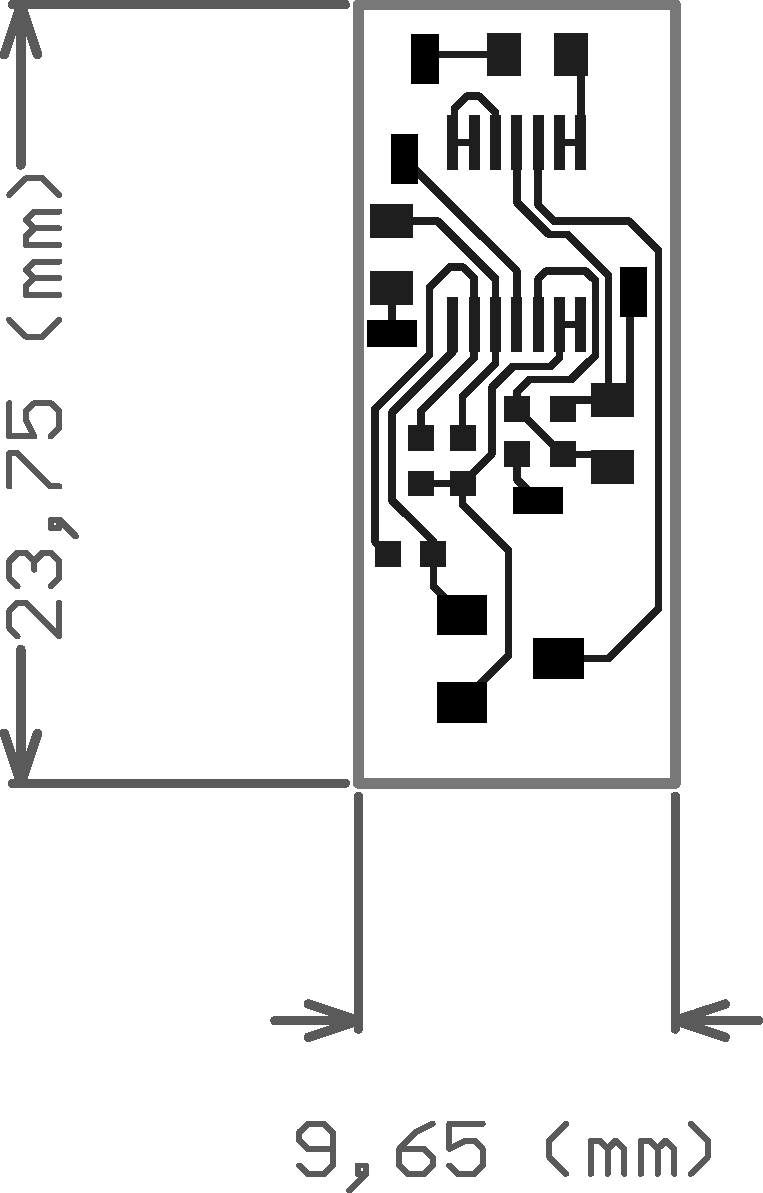
\includegraphics[width=0.2\textwidth]{PreAmp.pdf}
		\caption{The \gls{preamp} layout}
		\label{fig:preamp_layout}
\end{figure}

In \autoref{app:opamp_impedance} it is measured that $Z_i =$\SI{9.18}{\mega\ohm} which follows the assumption, but $Z_o$ is measured to \SI{9.06}{\kilo\ohm} which means that $R_V$ might have to be changed. 
 
\section{Description of the chosen DSP}

The chosen DSP is the Texas Instruments TMS320C5515 Fixed-Point Digital Signal Processor.

\subsection{Power}

The DSP processor gets its power from the \gls{usb} connection.

\subsection{Different Ports}

The C5515 features multiple ports and connectors. It has a micro SD connector, an expansion edge connector as well as a two \gls{usb}s. It also has an audio IN and two Bluetooth interfaces. \\

Each USB connector has a different role, one is used for software purposes and the other one to connect to the personal computer. 

\subsection{LCD Screen}

The \gls{dsp} processor has also an LCD screen that can print different characters by using a string of 14 pins. 

\subsection{Interface with the User}

The processor contains two switch buttons that can be integrated in the software to create an action. 

\subsection{Expansion}

The expansion connectors can be used to redirect the signals to other user interfaces that can be attached to some of the pins on the DSP. The exact number of the pins is in the data sheet. 

\subsection{Monitoring and Testing}

Several "Test points" are available in order to see the signals' behavior moving in the \gls{dsp} processor.

\subsection{Performance}

The \gls{dsp} can run on different speeds depending on how much the \gls{cpu} is powered. The clock rate can be between 60 and 75 MHz if powered with 1.05 Volts and between 100 and 120 MHz if powered with 1.3 Volts. \\

\subsection{Memory}

The chosen DSP has 320 \gls{kb} of \gls{ram} and 120 \gls{kb} of \gls{rom}. \\
There is also a 64 \gls{kb} of dual-access \gls{ram}, 256 \gls{kb} single-access \gls{ram} and 128 single access \gls{rom}. \\
Dual-access and single access \gls{ram}s presented above can be accessed using an internal program, data or \gls{dma} buses. \\
Dual-access and single access \gls{ram}s are divided into blocks that can be accessed using byte address ranges. Ranges are defined for each block but all blocks of a same memory type can be regrouped into one address range. \\
\gls{dma} address range for the block 0 of the dual-access \gls{ram} is 0001 0000h – 0001 1FFFh for instance. \\
All of the addresses are presented in the data sheet tables 2-2, 2-3.
The single-access \gls{rom} is also divided into blocks and has an address range. The usable range can be changed using a software. \\

The external memory interface permits a connection to other memories from other devices than the \gls{dsp}. 
\chapter{Design of the Different Effects}
\section{Design of the Chorus and Flanger Effect}

\subsection{Obtaining the Differential Equation}

The flanger- and chorus- effect are similar in their design so they will be presented in the same section. \\

From the block diagram presented in section \autoref{sec:chorus}, a block diagram in the discrete time domain for the flanger and chorus effect can be obtained and is shown in \autoref{fig:chorus_diag_des}. \\ 
The chorus effect is the one in red and black while the flanger is only in black.  
\begin{figure} [htbp!]
	\centering
\begin{picture}(0,0)%
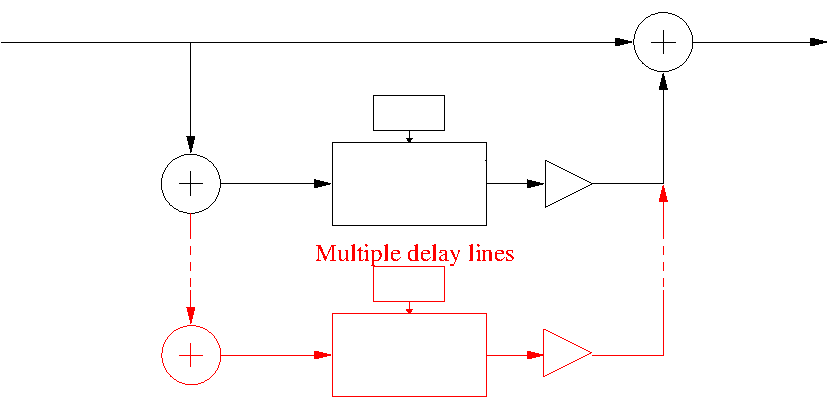
\includegraphics{chorus_diag_des.pdf}%
\end{picture}%
\setlength{\unitlength}{4144sp}%
%
\begingroup\makeatletter\ifx\SetFigFont\undefined%
\gdef\SetFigFont#1#2#3#4#5{%
	\reset@font\fontsize{#1}{#2pt}%
	\fontfamily{#3}\fontseries{#4}\fontshape{#5}%
	\selectfont}%
\fi\endgroup%
\begin{picture}(6327,3018)(3766,-3493)
\put(6571,-1906){\color[rgb]{0,0,0}$z^{-d_{1}}$}%

\put(8101,-1636){\color[rgb]{0,0,0}$g_{1}$}%

\put(6616,-3211){\color[rgb]{1,0,0}$z^{-d_{2}}$}%

\put(8101,-2986){\color[rgb]{1,0,0}$g_{2}$}%

\put(6706,-2671){\color[rgb]{1,0,0}\textit{LFO}}%

\put(6706,-1366){\color[rgb]{0,0,0}\textit{LFO}}%

\put(3781,-646){\color[rgb]{0,0,0}\textit{x[n]}}%

\put(9406,-646){\color[rgb]{0,0,0}\textit{y[n]}}%

\end{picture}%
\caption{Block Diagram of the chorus and flanger effect in the discrete time domain.}
\label{fig:chorus_diag_des}
\end{figure}

From \autoref{fig:chorus_diag_des}, the following differential equations can be inferred:

The equation for the flanger can be written as in \autoref{eq:flang_eq}
\begin{equation}
\label{eq:flang_eq}
		y[n] = x[n] + x[n- d_{1}] \cdot g_{1}  
\end{equation}

The equation for the chorus can be written as in \autoref{eq:chor_eq}:

\begin{equation}
\label{eq:chor_eq}
y[n] = x[n] + \sum_{j=1}^{i}  (x[n- d_{j}] \cdot g_{j})
\end{equation}

The index $i$ represents the number of delays that are being implemented in the chorus effect which is also the chorus size. Index $n$ represents the present sample. \\
If the implementation is done using a time varying delay, equations \ref{flang_eq} and \ref{chor_eq} can be re-written as \autoref{eq:flang_eq2} and \autoref{eq:chor_eq2}:

\begin{equation}
\label{eq:flang_eq2}
y[n] = x[n] + x[n- d_{1}[n]] \cdot g_{1}  
\end{equation}

\begin{equation}
\label{eq:chor_eq2}
y[n] = x[n] + \sum_{j=1}^{i}  (x[n- d_{j}[n]] \cdot g_{j})
\end{equation}

The delay value has to be a periodic function that is varying in a user-defined range. As illustrated in \autoref{fig:chorus_diag_des}, this varying delay can be made from a \gls{lfo}.

The LFO that makes the delay varies is a sine wave in the chorus and the flanger effect. In the case of the flanger, the user can set the LFO frequency between 0,1 and 10 Hz and only the boundaries for the chorus. \\

The gain for the flanger effect can be chosen by the user. For the chorus, the user can choose the boundaries of the gain value that will be randomly selected for each of the delay lines. \\

The number of delay lines for the chorus effect is also a choice but should not exceed 4, the reason is that after 4 lines it has been found that the effect has a strange sound. \\

The delay time for the flanging effect should be between 1 and 20 ms while the delay time in the chorus should be longer than 20ms. \\

From the difference equation, it can be seen that the design is using a FIR Comb filter but where the delay value varies. \todo[inline]{Why is it FIR comb filter?}

\subsection{Making the LFO by Cordic algorithm}
The \gls{lfo} in both the chorus- and the flanger- effect should, as stated in \autoref{}, be able to make sine waves from \SI{0.1}{\kilo\hertz} to \SI{10}{\kilo\hertz}. A \gls{dsp} is not necessarily able to calculate sine values and therefore an algorithm has to be implemented in order to make this possible. A way to do this is by using the \gls{cordic} algorithm, which can be used to calculate both sine, cosine, square roots etc \citep{cordic}. 
When using the \gls{cordic} algorithm for for an \gls{lfo} the two equations \autoref{eq:cordic_x} and \autoref{eq:cordic_y} are almost all what is needed.

\begin{equation}
\label{eq:cordic_x}
		x_{n+1} = x_n \cdot \cos(\theta) - y_n \cdot \cdot \sin(\theta) 
\end{equation}
\startexplain
     \explain{$x_{n+1}$ is the present cosine value.}{\si{1}}
     \explain{$x_n$ is the previous cosine value.}{\si{1}}
     \explain{$y_n$ is the previous sine value.}{\si{1}}
     \explain{$yn$ is the index.}{\si{1}}
    \stopexplain 

\begin{equation}
\label{eq:cordic_y}
		y_{n+1} = y_n \cdot \cos(\theta) + x_n \cdot \sin(\theta) 
\end{equation}
\startexplain
     \explain{$y_{n+1}$ is the present sine value.}{\si{1}}
\stopexplain

The algorithm works by initializing $x_0$ to 1 and $y_0$ to 0. This way $x_1$ becomes equal to $\cos(\theta)$ and $y_1$ becomes equal to $\sin(\theta)$. When the next iteration begins, the initial vector will then have the coordinates [$x_1$, $y_1$]. This way $x_2$ becomes equal to $\cos(2 \cdot \theta)$ and $y_2$ becomes equal to $\sin(2 \cdot \theta)$. Thus it is only necessary to calculate $\cos(\theta)$ and $\sin(\theta)$ and then follow the iterations to produce a sine wave. The frequency of the sine wave is decided by $\theta$. The relation between the frequency and $\theta$ is shown in \autoref{eq:cordic_freq}.

\begin{equation}
\label{eq:cordic_freq}
		\theta = 2 \cdot \pi \cdot \frac{F}{F_s} 
\end{equation}
\startexplain
     \explain{$F$ is the wanted frequency of the sine wave.}{\si{\hertz}}
     \explain{$F_s$ is the sampling frequency.}{\si{\hertz}}
\stopexplain 

This way the \gls{cordic} algorithm will have $\frac{F_s}{F}$ steps round the unitcircle and thereby produce a sine wave with frequency $F$ and sine values between $\pm$1.
A MATLAB simulation of the \gls{cordic} algorithm was made and set to produce a \SI{10}{\hertz} sine wave. The result of the simulation is shown in \autoref{}.

\begin{figure}[!h]
    \centering
        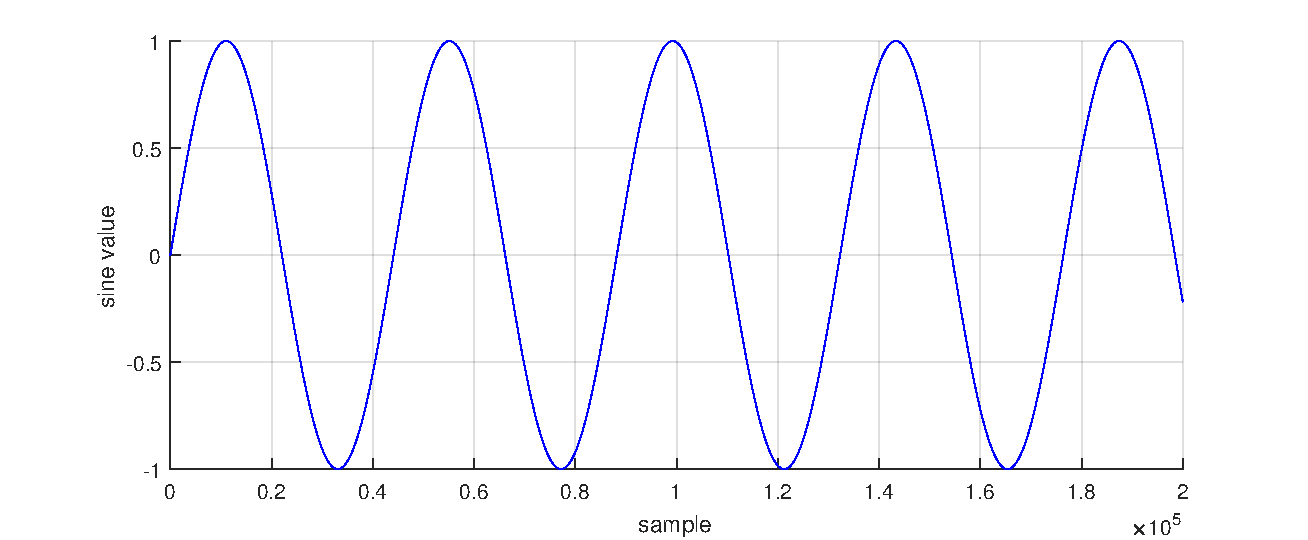
\includegraphics[width=0.5\textwidth]{cordic_1Hz.pdf}
        \caption{Simulation of the \gls{cordic} algorithm, set to produce a \SI{10}{\hertz} sine wave.}
        \label{fig:cordic_10Hz}
  \end{figure}
  
When implementing the \gls{cordic} algorithm on a \gls{dsp}, a gain value smaller than 1, might have to be implemented in \autoref{eq:cordic_x} and \autoref{eq:cordic_y} on $x_n$ and $y_n$ to make the algorithm stable. 







\subsection{Matlab Simulation}

A delay can be done in different ways digitally. One way is to use a ring buffer also known as circular buffer. \\
The idea of this data structure is that it takes values and only outputs them when it gets full, and overwrites the oldest after outputting it. It is a kind of a FIFO queue structure but where the start and the overwriting can start at any index. \\
This means that the size of the buffer depends on the delay.  The buffer size must then be always up-to-date with the new delay value. \\ 
The value of the delay is determined by a periodic function as said before, different waveforms can be used as said in \autoref{chor_flang}. A common periodic function that can be used is the sine. Since it varies between 0 and 1, it can be then multiplied with the user-defined range. 
The delay can then be written as:

\begin{equation}
	d[n]= A \cdot sin(2\pi  \cdot \frac{f_{l}}{f_{s}} n)
\end{equation}

\startexplain
     \explain{$A$ is the value of the user-defined range which is also the depth.}{\si{1}}
     \explain{$f_{s}$ the sampling frequency.}{\si{\hertz}}
     \explain{$f_{l}$ is the frequency of the \gls{lfo}.}{\si{\hertz}}
    \stopexplain 

The Matlab code for the flanger effect is:

\begin{lstlisting}[language=Matlab, caption= Matlab code for flanger effect]

%Flanger Effect
%Group 641
%Mohamed Gabr, Jonas and Sebastian


filename = 'inputttt.wav'; 
%The filename is inserted here, should be in the same directory as the
%codefile.
[input, fs] = audioread(filename, 'native');
%input samples and sample rate are extracted from the file.
input = input / (max(abs(input)));
%the input is rescaled in order to have values between -1 and 1. 
fl = 100;  
%LFO Frequency is chosen here.
sample_no = length(input); 
%Length of the input samples table.
g = 100; 
%Gain
delay_s = 0.0050; 
% The maximum delay in seconds.
after_delay = (1:1:sample_no); 
before_delay = (1:1:sample_no);
output = (1:1:sample_no);
%Needed tables in the code are intialized to make the code faster.
disp('max delay')
max_delay = delay_s * fs  
%Convert the maximum delay from delay in seconds to delay in samples.

buffer = zeros(1,abs(round(max_delay))); 
%intializing the buffer array.

for i = 1:1:sample_no  %Loop that treats a sample per iteration. 
 delay = max_delay * cos(2*pi*i*(fl/fs)); %Calculate time varying delay 
 %(unit is samples)
 buffer = [buffer(2:end) input(i)]; 
 %move the values in the buffer ==> first value overwritten, one new 
 %value added at the end.
 if abs(delay) < 1   %All delay values less than zero are considered as
  %not having a delay
  after_delay(i) = 0;
 else
  if floor(delay) == delay || abs(floor(delay)) >= floor(max_delay)
   after_delay(i) = buffer(round(abs(delay))) * g;
   %Treating the case when the delay is an integer and when it has a
   %value bigger than the maximum delay. 
  else %Treating the case when the delay is not an integer
   x1 = abs(floor(delay));
   x2 = x1 + 1;
   y1 = buffer(x1);
   y2 = buffer(x2);
   coeff = (y1 - y2)/(x1 - x2);
   %Making a linear approximation between the samples to increase
   %precision
   after_delay(i) = delay * coeff * g;  %sound from the delay line
   %in the block diagram 
  end
 end
 before_delay(i) = input(i);  %sound from the direct line
 output(i) = after_delay(i) + before_delay(i); %output delayed signal 
end
output = output / max(abs(output)); %output is rescaled to values between
% -1 and 1 to avoid clipping. 
audiowrite('out_flan.wav',output,fs); %Writing the values in a file, 
% PS: audiowrite will clip if the values are not between -1 and 1. 
plot(output,'r') %plotting the output samples in red.
hold on
grid
plot(before_delay,'b') %plotting the input samples in blue on the same fig.




\end{lstlisting}


The code is commented for the user's instruction.\\

The Matlab code for the chorus effect is:

\begin{lstlisting}[language=Matlab, caption= Matlab code for chorus effect]

%Chorus Effect
%Group 641
%Mohamed, Jonas and Sebastian

filename = 'inputttt.wav'; %Typing the filename, should be in same 
%directory as the codefile
[input, fs] = audioread(filename);
%input samples and sample rate are extracted from the file.
input = input / (max(abs(input)));
%the input is rescaled in order to have values between -1 and 1.
lines = 5; %number of chorus lines 
fl = randi(10,1,lines);
%LFO Frequencies for each line are generated.
delay = (1:1:lines);
%Delay table generated here to speed the coding. 
sample_no = length(input); 
%Length of the input samples
g = rand(1,lines); 
%Gain values generated here
delay_s = 0.025; 
% Maximum delay in seconds 
after_delay = rand(lines, sample_no); 
before_delay = (1:1:sample_no);
output = (1:1:sample_no);
% Generating tables to speed the code. 
max_delay = delay_s * fs  
%convert the delay from delay in seconds to delay in samples. 


buffer = zeros(1,abs(round(max_delay))); %create the buffer array 

for i = 1:1:sample_no %loop that gives one output sample per iteration
 buffer = [buffer(2:end) input(i)]; %moving buffer values
 before_delay(i) = input(i); %Value before delay
 output(i) = before_delay(i); %adding it to one output sample
 for j = 1:1:lines %Generating delays and then samples after delay for 
 %each chorus line
   delay(j) = max_delay * cos(2*pi*i*(fl(j)/fs)); %Calculate time  
   %varying delay (unit is samples)
   if abs(delay(j)) < 1 %Treating the case where the delay is less 
   %than one.
	 after_delay(j,i) =0;
   else
	 if floor(delay(j)) == delay(j) || abs(floor(delay(j))) >= floor(max_delay)
	   after_delay(j,i) = buffer(round(abs(delay(j)))) * g(j);
	   %Treating the case when the delay is an integer and when it has a
	   %value bigger than the maximum delay. 
	 else  %Treating the case when the delay is not an integer
	   x1 = abs(floor(delay(j)));
	   x2 = x1 + 1;
	   y1 = buffer(x1);
	   y2 = buffer(x2);
	   coeff = (y1 - y2)/(x1 - x2);
	   %Making a linear approximation between the samples to increase
	   %precision
	   after_delay(j,i) = delay(j) * coeff * g(j);  
	   %sound from the delay line in the block diagram
	 end
   end
   output(i) = output(i) + after_delay(j,i);
   %Signal output sample
 end
end
output = output / max(abs(output)); %output is rescaled to values between
% -1 and 1 to avoid clipping. 
audiowrite('out_chor.wav',output,fs); %Writing the values in a file, 
% PS: audiowrite will clip if the values are not between -1 and 1.
plot(output,'r') %plotting the output samples in red.
hold on
grid
plot(before_delay,'b') %plotting the input samples in blue on the same fig.



\end{lstlisting}

The codes where simulated on different audiofiles. 



%%
\part{Tests}\label{pt:tests} 
%%
\part{Conclusions}\label{pt:conclusions} 
%

\glsresetall
\appendix % Start of appendix
\addtocontents{toc}{\protect\setcounter{tocdepth}{0}} 
%\input{chapters/appendices/_appendices} % Include appendices
%Appendix:

 \graphicspath{{figures/appendix/}}
%\part{Appendix}\label{pt:appendix}
\chapter{Test a guitars frequency area}\label{app:frequency_area}
A test was made to get a view of the frequency area, in which the tones from a guitar lies.

\section*{Materials and setup}
To measure the frequency area on a guitar, the following materials are used:
\begin{itemize}
\item Digilent Analog Discovery 2 (Oscilloscope)
\item Fender Squier Classic Vibe Telecaster (Guitar)
\item Digilent Waveforms 2015 (PC - software)
\end{itemize}

\begin{figure}[htbp!]
\centering
\def\svgwidth{\columnwidth}
\chapter{Test a guitars frequency area}\label{app:frequency_area}
A test was made to get a view of the frequency area, in which the tones from a guitar lies.

\section*{Materials and setup}
To measure the frequency area on a guitar, the following materials are used:
\begin{itemize}
\item Digilent Analog Discovery 2 (Oscilloscope)
\item Fender Squier Classic Vibe Telecaster (Guitar)
\item Digilent Waveforms 2015 (PC - software)
\end{itemize}

\begin{figure}[htbp!]
\centering
\def\svgwidth{\columnwidth}
\chapter{Test a guitars frequency area}\label{app:frequency_area}
A test was made to get a view of the frequency area, in which the tones from a guitar lies.

\section*{Materials and setup}
To measure the frequency area on a guitar, the following materials are used:
\begin{itemize}
\item Digilent Analog Discovery 2 (Oscilloscope)
\item Fender Squier Classic Vibe Telecaster (Guitar)
\item Digilent Waveforms 2015 (PC - software)
\end{itemize}

\begin{figure}[htbp!]
\centering
\def\svgwidth{\columnwidth}
\input{figures/appendix/guitar_frequency_test.pdf_tex}
\caption{Setup for measuring frequency area on a guitar.}
		\label{fig:appendix:guitar_freq}
\end{figure}

\section*{Test procedure}
To the frequency area on a guitar, the following steps are made:
\begin{enumerate}
\item The materials are set up as in \autoref{fig:appendix:guitar_freq}.
\item Digilent Waveforms 2015 is set as a spectrum analyser. 
\item The guitar is set to use the neck pickup and the volume control and the tone control are turned all the way up.
\item The highest and the lowest tone on the guitar are played, measured by the oscilloscope and analysed in Digilent Waveforms 2015.
\item The guitar is set to use the bridge pickup and step 4 is repeated. 
\item The data is plotted in MATLAB.
\end{enumerate}

\section*{Results}

\begin{figure}[htbp!]
	\centering
		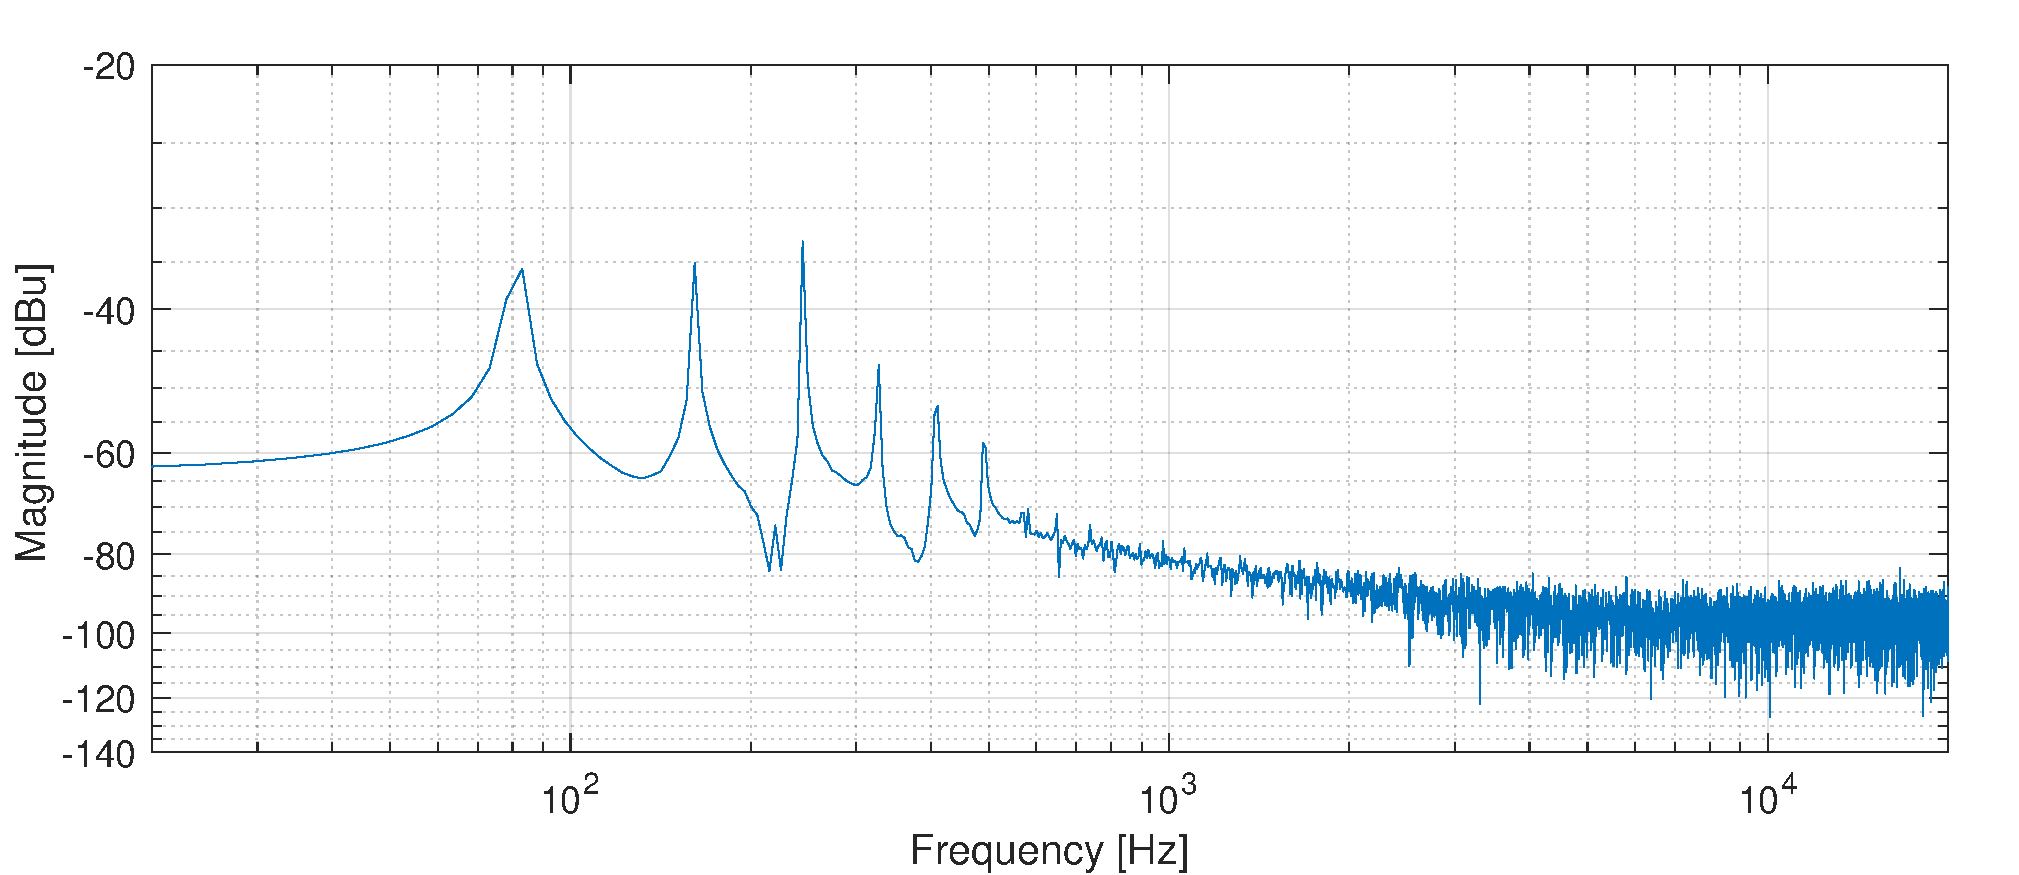
\includegraphics[width=1\textwidth]{guitar_low_E_neck.pdf}
		\caption{Measurement of the low E note on the neck pickup.}
		\label{fig:appendix:low_E_neck}
\end{figure}

On  \autoref{fig:appendix:low_E_neck} it is seen that the lowest significant frequency is around \SI{80}{\hertz} and the highest significant frequency is around \SI{400}{\hertz}, when playing the low E note on the guitar, using the neck pickup.

\begin{figure}[htbp!]
	\centering
		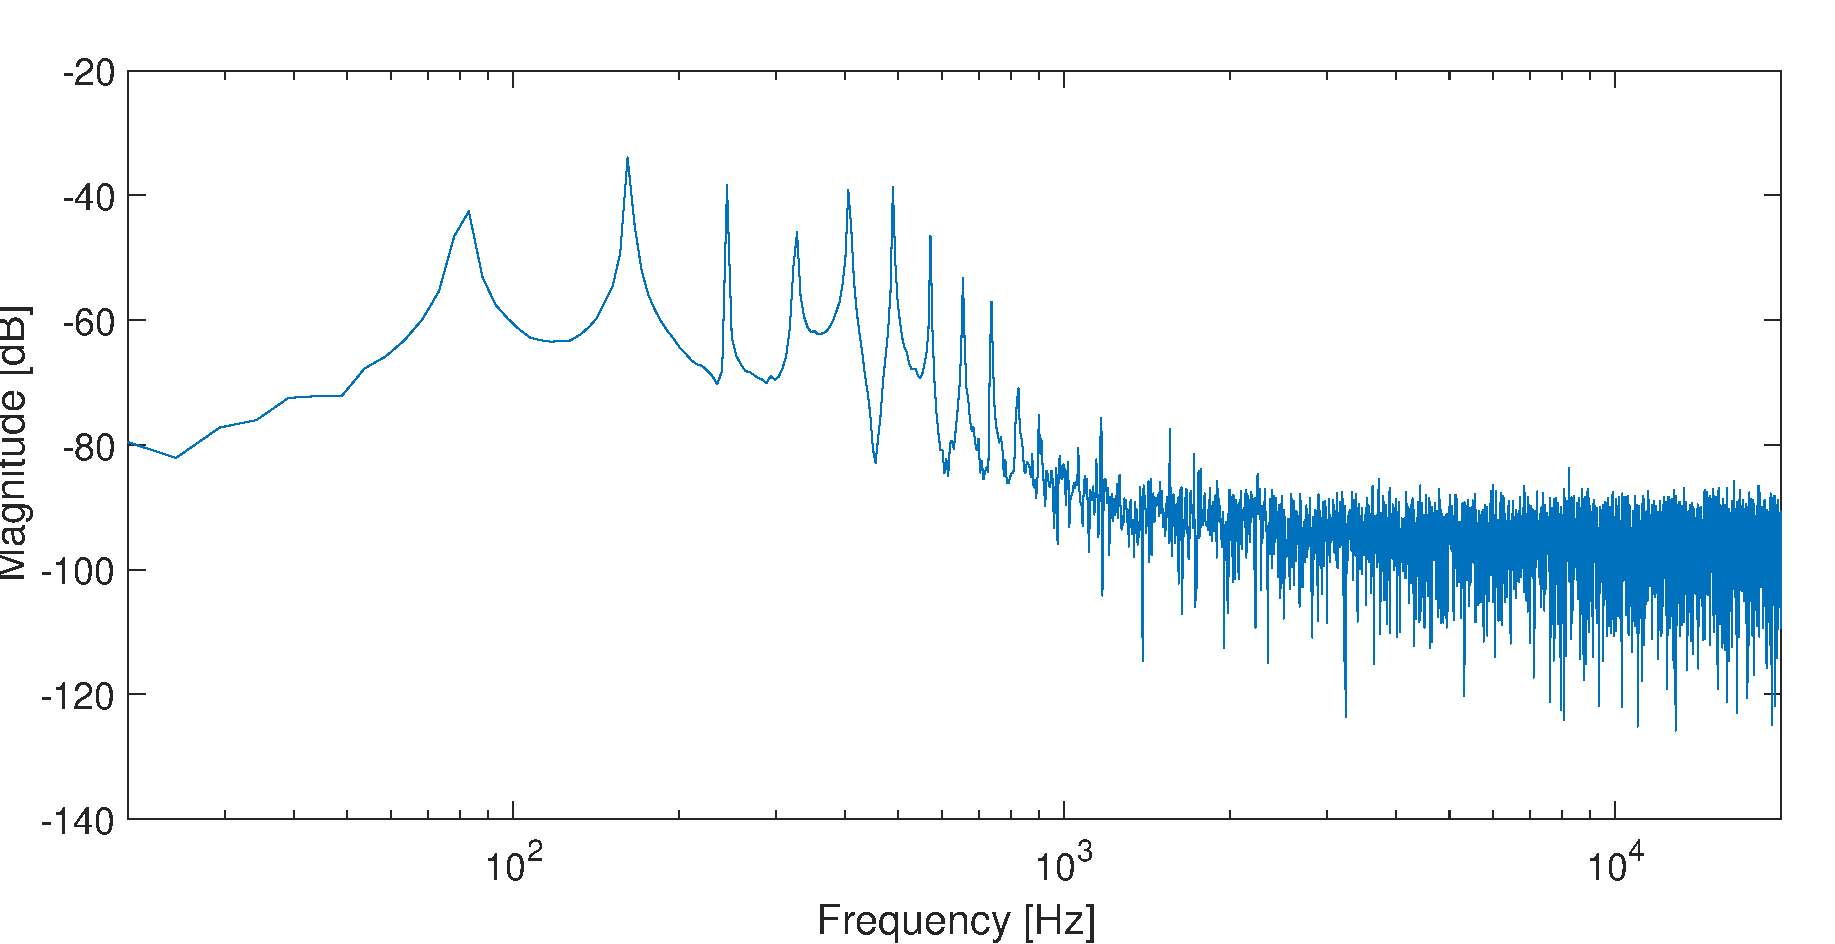
\includegraphics[width=1\textwidth]{guitar_low_E_bridge.pdf}
		\caption{Measurement of the low E note on the bridge pickup.}
		\label{fig:appendix:low_E_bridge}
\end{figure}

On  \autoref{fig:appendix:low_E_bridge} it is seen that the lowest significant frequency is around \SI{80}{\hertz} and the highest significant frequency is around \SI{730}{\hertz}, when playing the low E note on the guitar, using the bridge pickup.

\begin{figure}[htbp!]
	\centering
		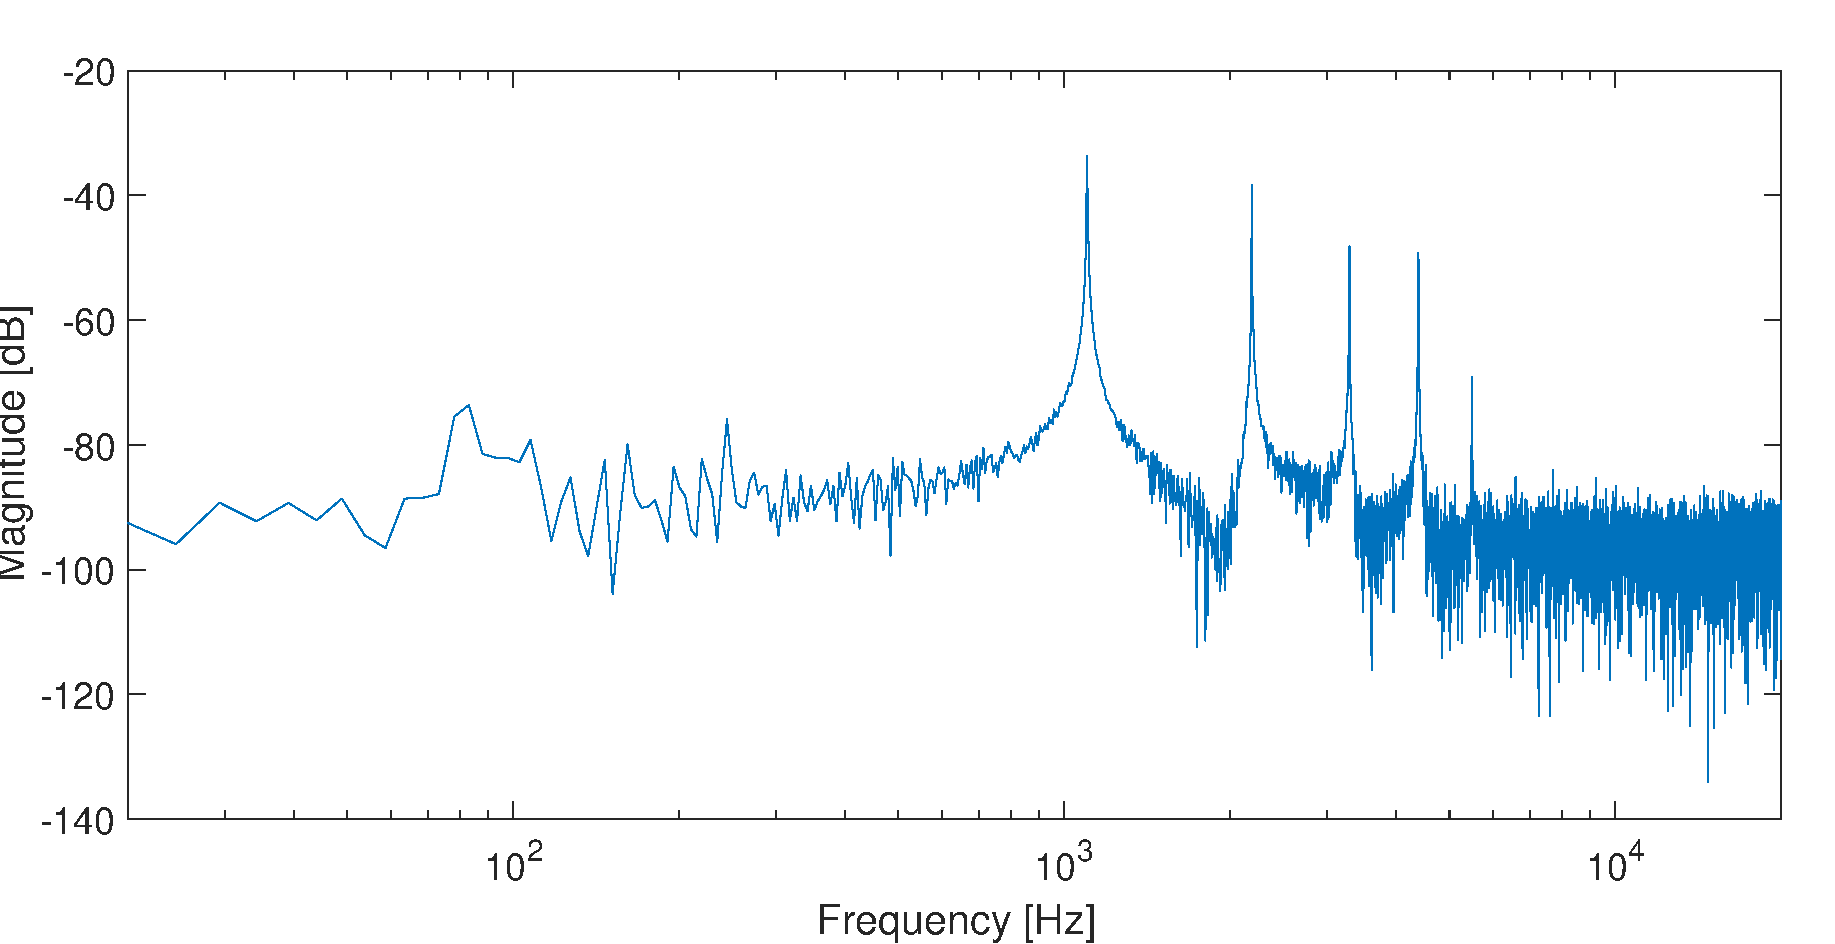
\includegraphics[width=1\textwidth]{guitar_high_Cis_neck.pdf}
		\caption{Measurement of the high C\# note on the neck pickup.}
		\label{fig:appendix:high_Cis_neck}
\end{figure}

On  \autoref{fig:appendix:high_Cis_neck} it is seen that the lowest significant frequency is around \SI{1100}{\hertz} and the highest significant frequency is around \SI{4400}{\hertz}, when playing the high C\# note on the guitar, using the neck pickup.

\begin{figure}[htbp!]
	\centering
		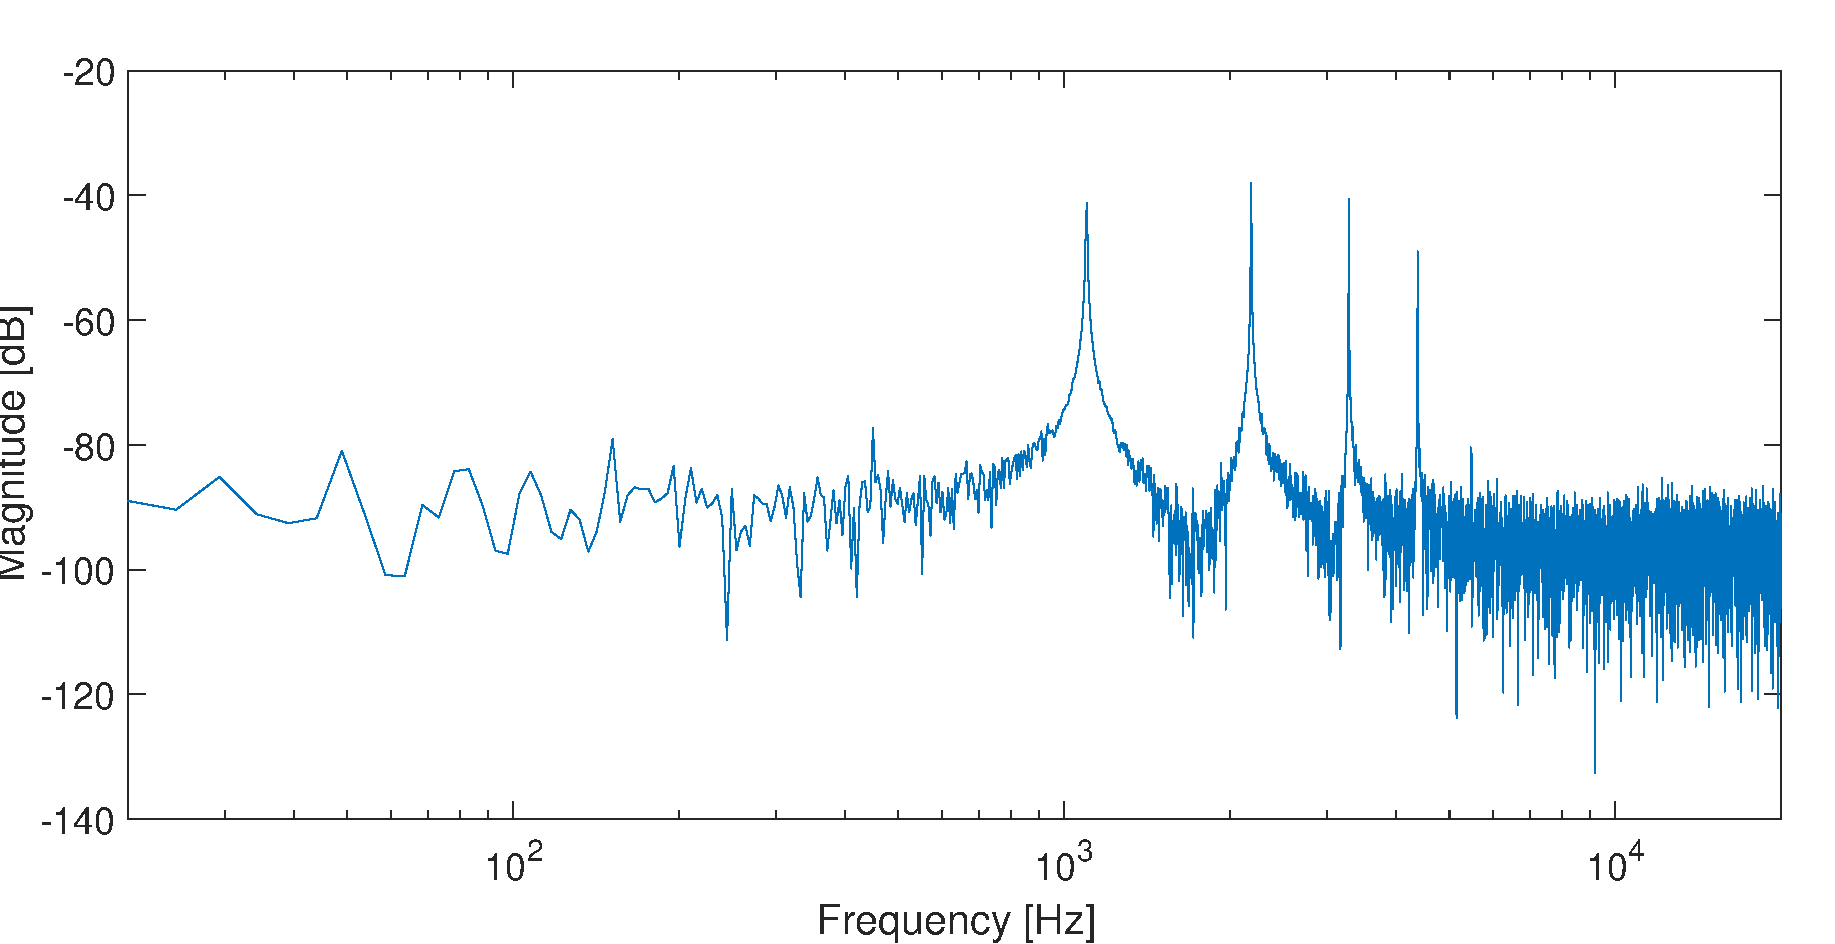
\includegraphics[width=1\textwidth]{guitar_high_Cis_bridge.pdf}
		\caption{Measurement of the high C\# note on the bridge pickup.}
		\label{fig:appendix:high_Cis_bridge}
\end{figure}

On  \autoref{fig:appendix:high_Cis_bridge} it is seen that the lowest significant frequency is around \SI{1100}{\hertz} and the highest significant frequency is around \SI{4400}{\hertz}, when playing the high C\# note on the guitar, using the bridge pickup. 

\begin{figure}[htbp!]
	\centering
		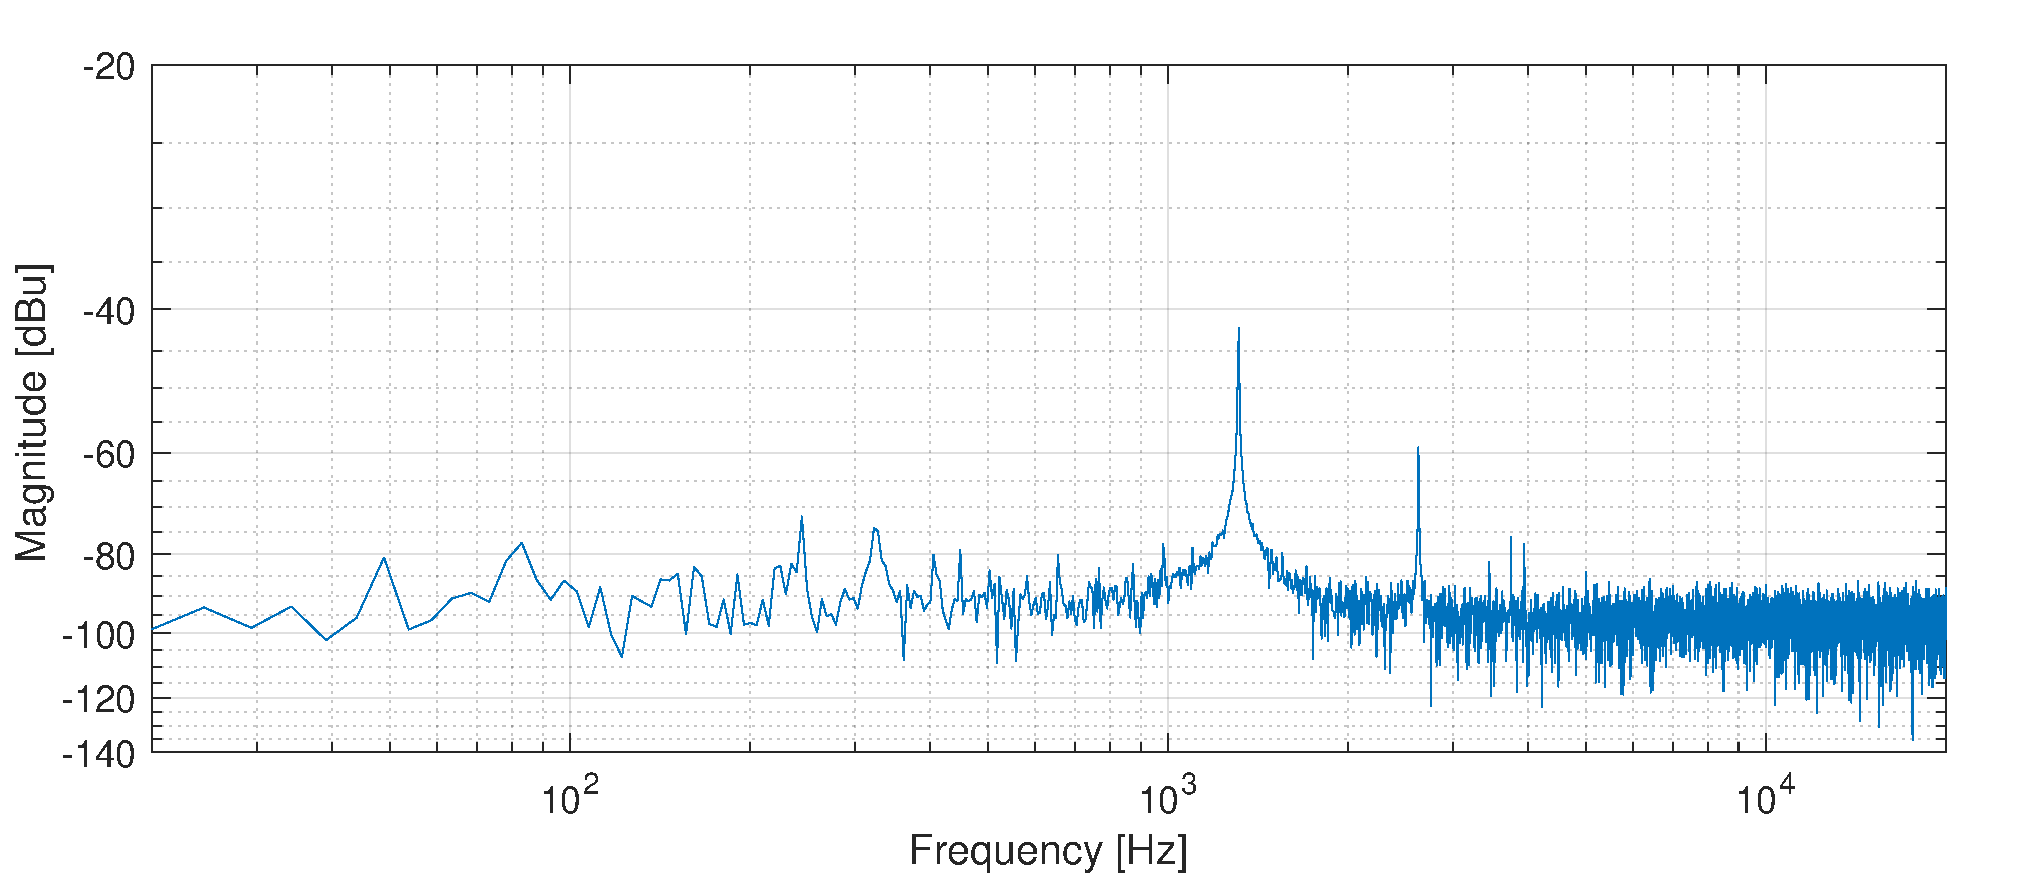
\includegraphics[width=1\textwidth]{guitar_high_E_flasholet_bridge.pdf}
		\caption{Measurement of the high E note, played as flasholet, on the bridge pickup.}
		\label{fig:appendix:high_E_bridge_flasholet}
\end{figure}

On  \autoref{fig:appendix:high_E_bridge_flasholet} it is seen that the lowest significant frequency is around \SI{1300}{\hertz} and the highest significant frequency is around \SI{2600}{\hertz}, when playing the high E note on the guitar as flasholet, using the bridge pickup. 

\caption{Setup for measuring frequency area on a guitar.}
		\label{fig:appendix:guitar_freq}
\end{figure}

\section*{Test procedure}
To the frequency area on a guitar, the following steps are made:
\begin{enumerate}
\item The materials are set up as in \autoref{fig:appendix:guitar_freq}.
\item Digilent Waveforms 2015 is set as a spectrum analyser. 
\item The guitar is set to use the neck pickup and the volume control and the tone control are turned all the way up.
\item The highest and the lowest tone on the guitar are played, measured by the oscilloscope and analysed in Digilent Waveforms 2015.
\item The guitar is set to use the bridge pickup and step 4 is repeated. 
\item The data is plotted in MATLAB.
\end{enumerate}

\section*{Results}

\begin{figure}[htbp!]
	\centering
		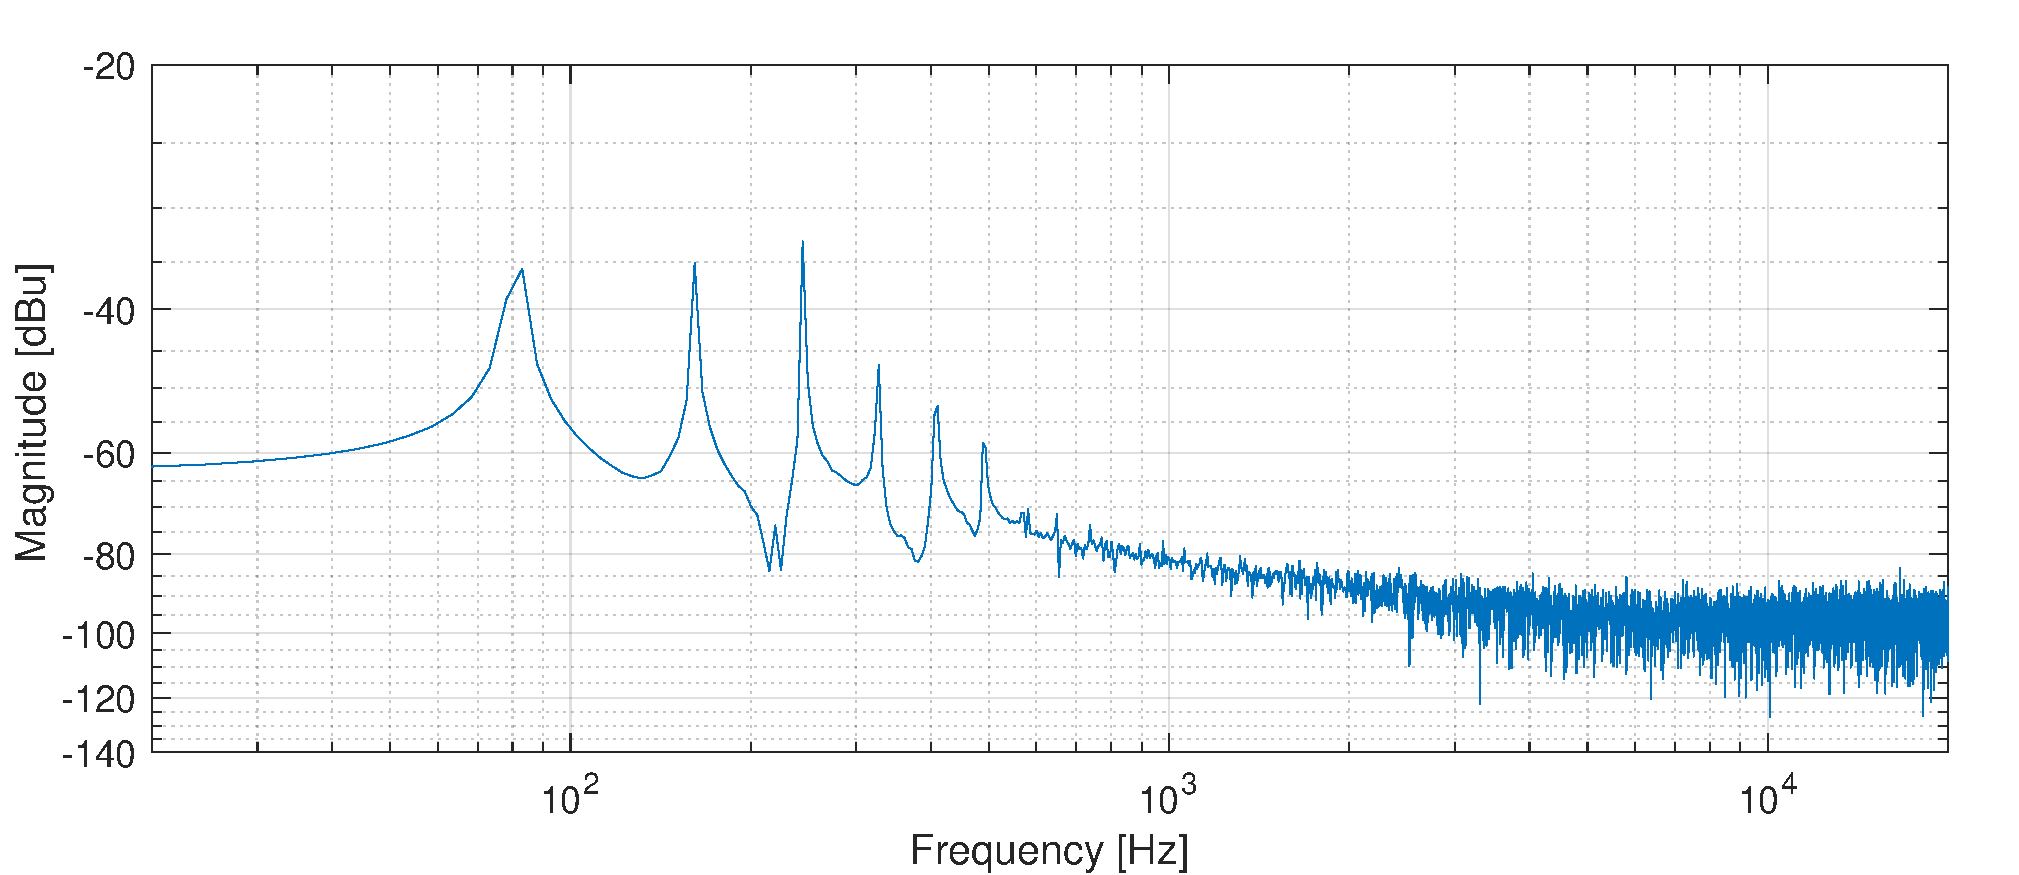
\includegraphics[width=1\textwidth]{guitar_low_E_neck.pdf}
		\caption{Measurement of the low E note on the neck pickup.}
		\label{fig:appendix:low_E_neck}
\end{figure}

On  \autoref{fig:appendix:low_E_neck} it is seen that the lowest significant frequency is around \SI{80}{\hertz} and the highest significant frequency is around \SI{400}{\hertz}, when playing the low E note on the guitar, using the neck pickup.

\begin{figure}[htbp!]
	\centering
		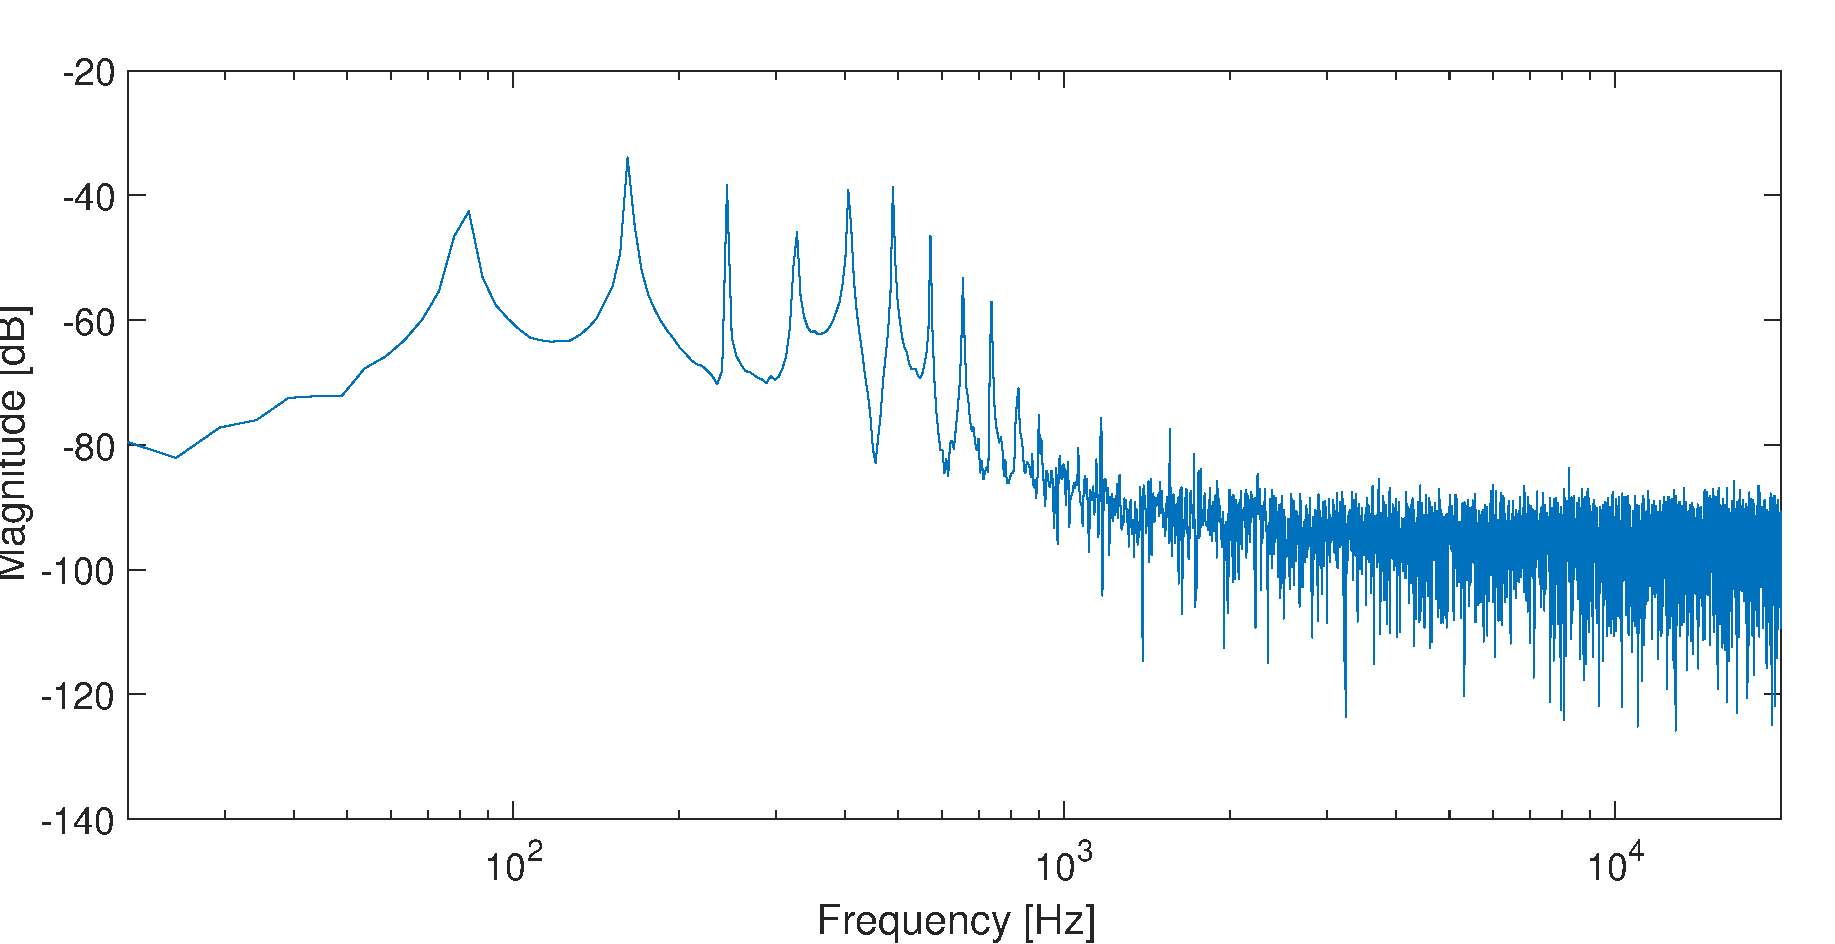
\includegraphics[width=1\textwidth]{guitar_low_E_bridge.pdf}
		\caption{Measurement of the low E note on the bridge pickup.}
		\label{fig:appendix:low_E_bridge}
\end{figure}

On  \autoref{fig:appendix:low_E_bridge} it is seen that the lowest significant frequency is around \SI{80}{\hertz} and the highest significant frequency is around \SI{730}{\hertz}, when playing the low E note on the guitar, using the bridge pickup.

\begin{figure}[htbp!]
	\centering
		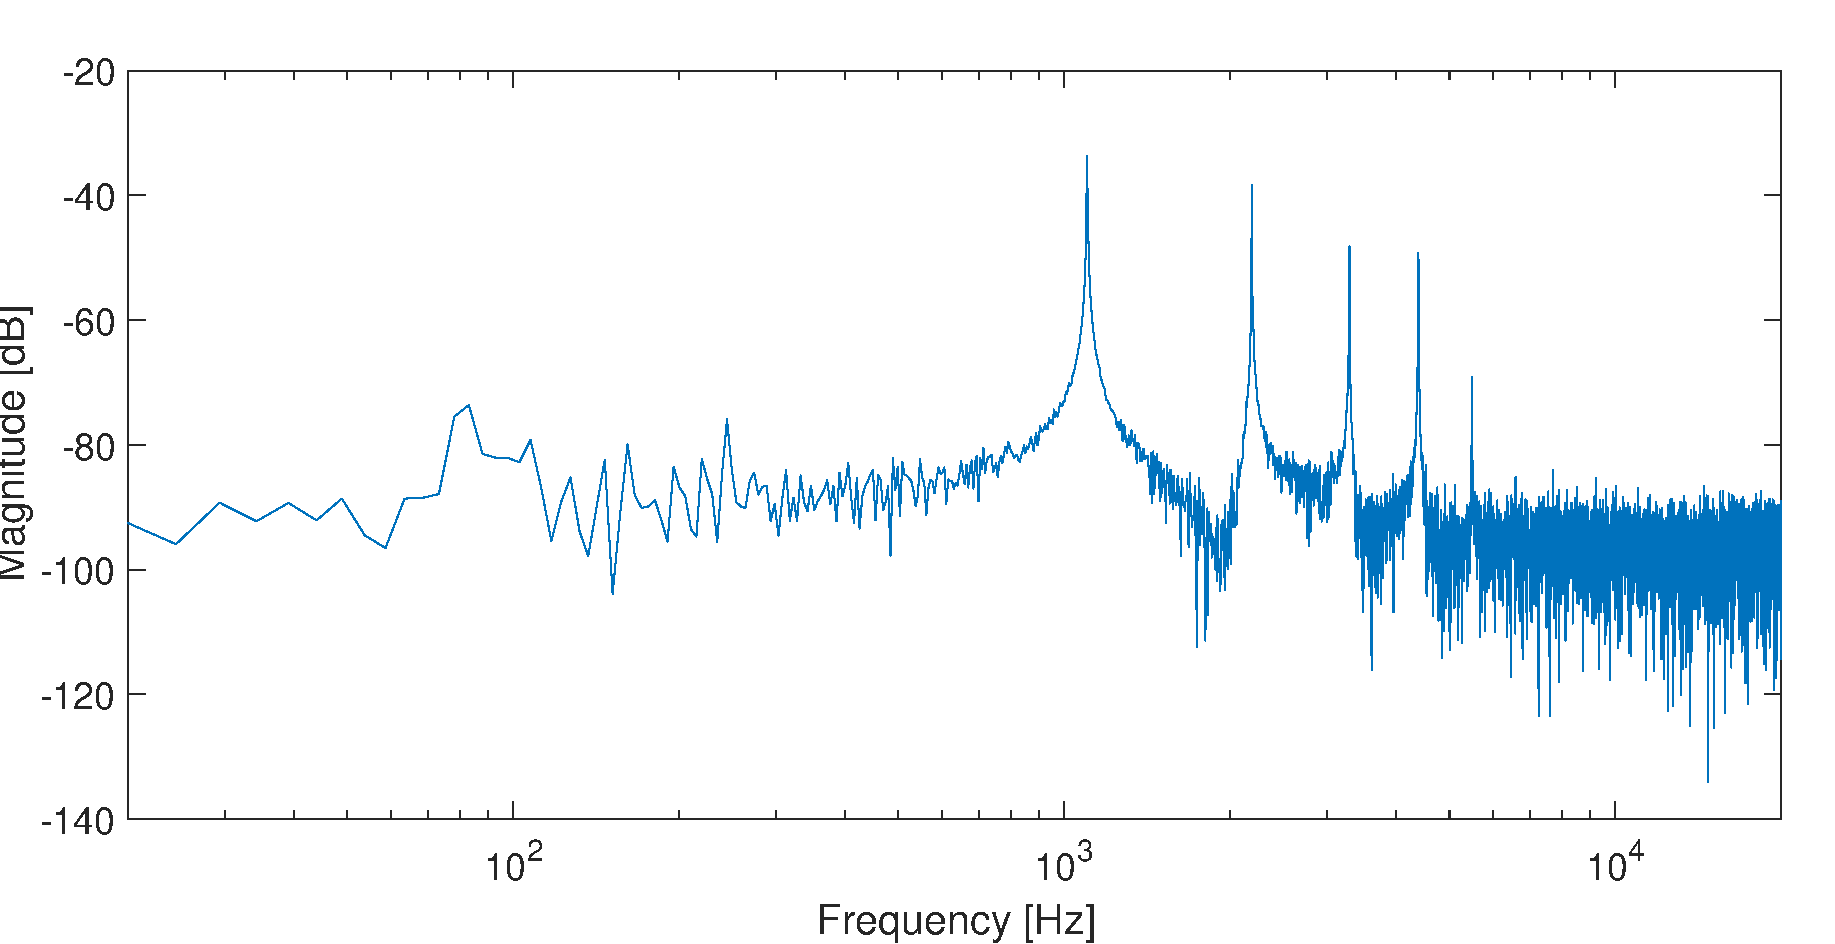
\includegraphics[width=1\textwidth]{guitar_high_Cis_neck.pdf}
		\caption{Measurement of the high C\# note on the neck pickup.}
		\label{fig:appendix:high_Cis_neck}
\end{figure}

On  \autoref{fig:appendix:high_Cis_neck} it is seen that the lowest significant frequency is around \SI{1100}{\hertz} and the highest significant frequency is around \SI{4400}{\hertz}, when playing the high C\# note on the guitar, using the neck pickup.

\begin{figure}[htbp!]
	\centering
		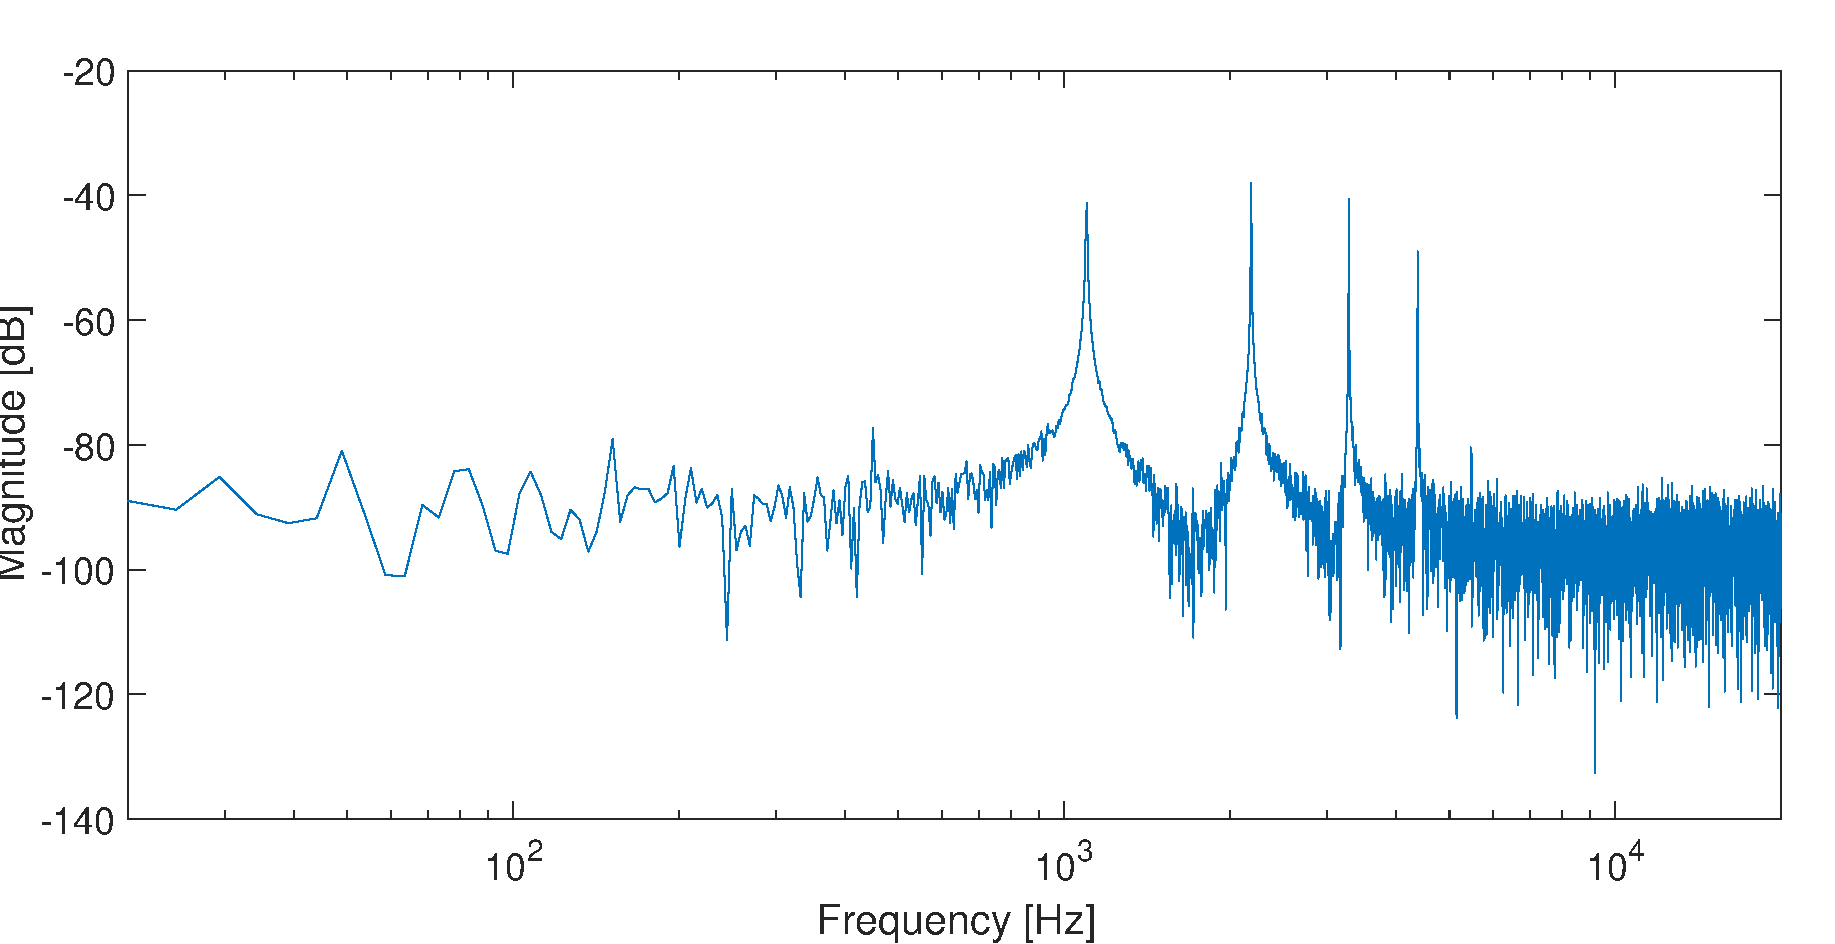
\includegraphics[width=1\textwidth]{guitar_high_Cis_bridge.pdf}
		\caption{Measurement of the high C\# note on the bridge pickup.}
		\label{fig:appendix:high_Cis_bridge}
\end{figure}

On  \autoref{fig:appendix:high_Cis_bridge} it is seen that the lowest significant frequency is around \SI{1100}{\hertz} and the highest significant frequency is around \SI{4400}{\hertz}, when playing the high C\# note on the guitar, using the bridge pickup. 

\begin{figure}[htbp!]
	\centering
		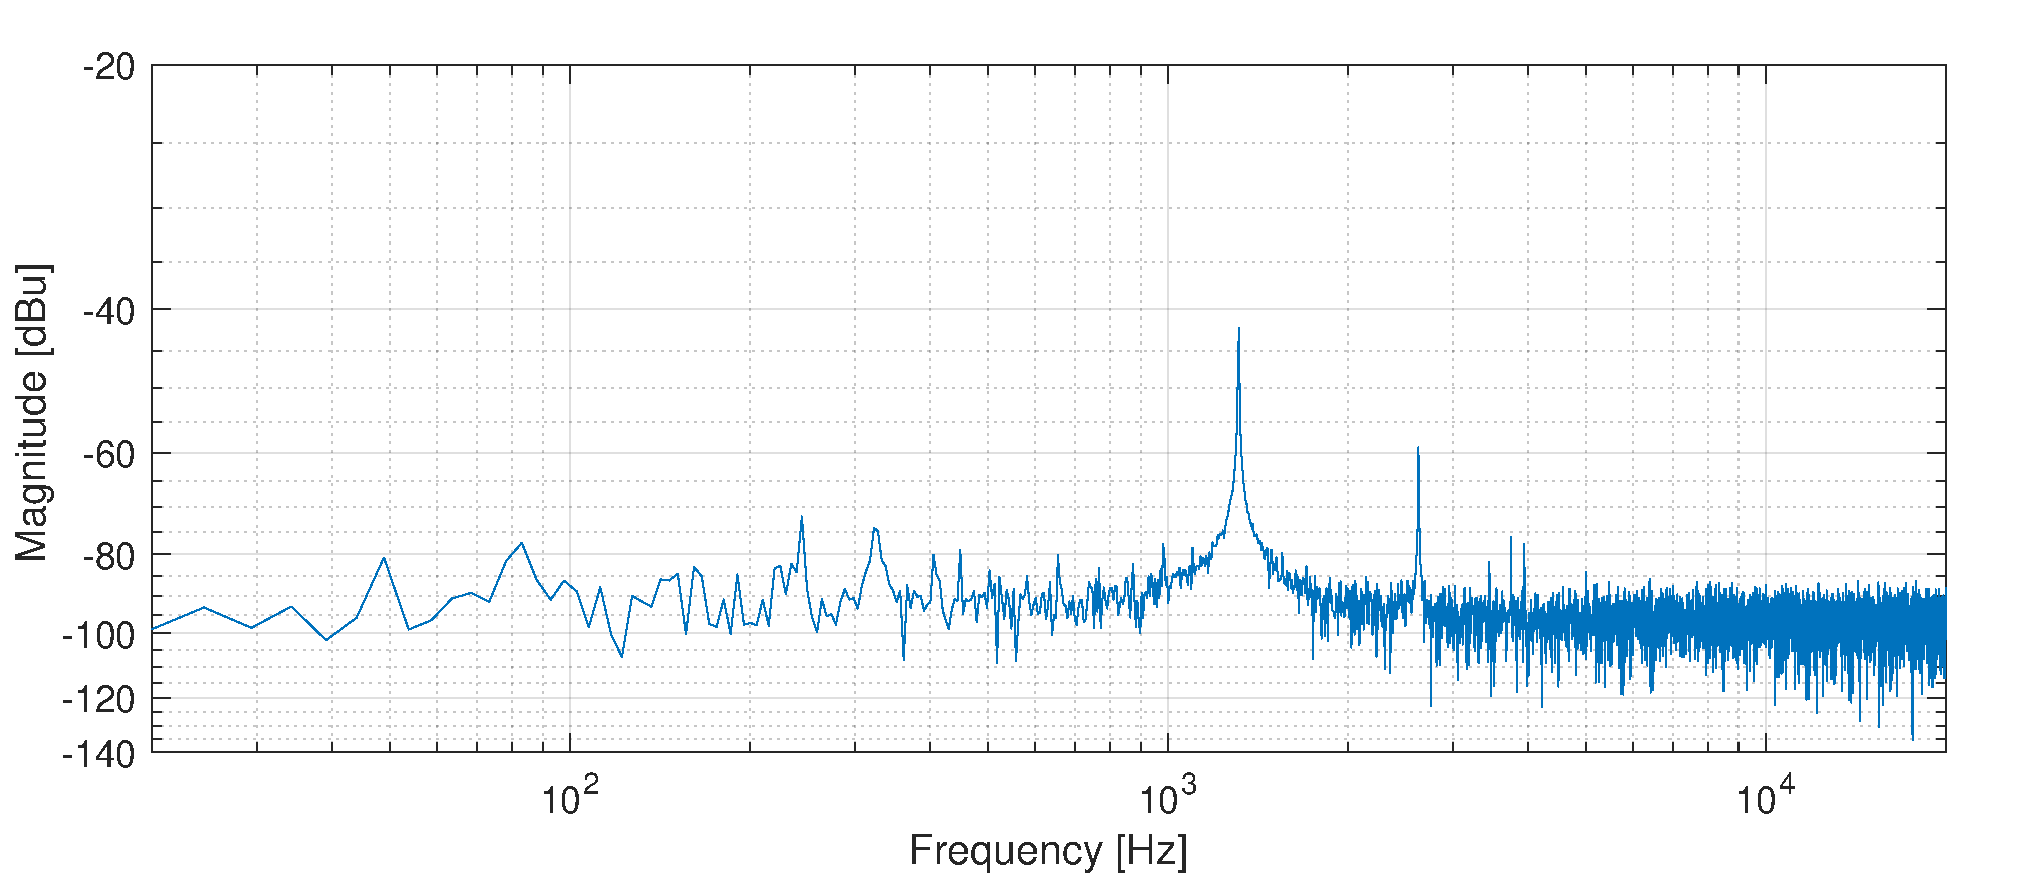
\includegraphics[width=1\textwidth]{guitar_high_E_flasholet_bridge.pdf}
		\caption{Measurement of the high E note, played as flasholet, on the bridge pickup.}
		\label{fig:appendix:high_E_bridge_flasholet}
\end{figure}

On  \autoref{fig:appendix:high_E_bridge_flasholet} it is seen that the lowest significant frequency is around \SI{1300}{\hertz} and the highest significant frequency is around \SI{2600}{\hertz}, when playing the high E note on the guitar as flasholet, using the bridge pickup. 

\caption{Setup for measuring frequency area on a guitar.}
		\label{fig:appendix:guitar_freq}
\end{figure}

\section*{Test procedure}
To the frequency area on a guitar, the following steps are made:
\begin{enumerate}
\item The materials are set up as in \autoref{fig:appendix:guitar_freq}.
\item Digilent Waveforms 2015 is set as a spectrum analyser. 
\item The guitar is set to use the neck pickup and the volume control and the tone control are turned all the way up.
\item The highest and the lowest tone on the guitar are played, measured by the oscilloscope and analysed in Digilent Waveforms 2015.
\item The guitar is set to use the bridge pickup and step 4 is repeated. 
\item The data is plotted in MATLAB.
\end{enumerate}

\section*{Results}

\begin{figure}[htbp!]
	\centering
		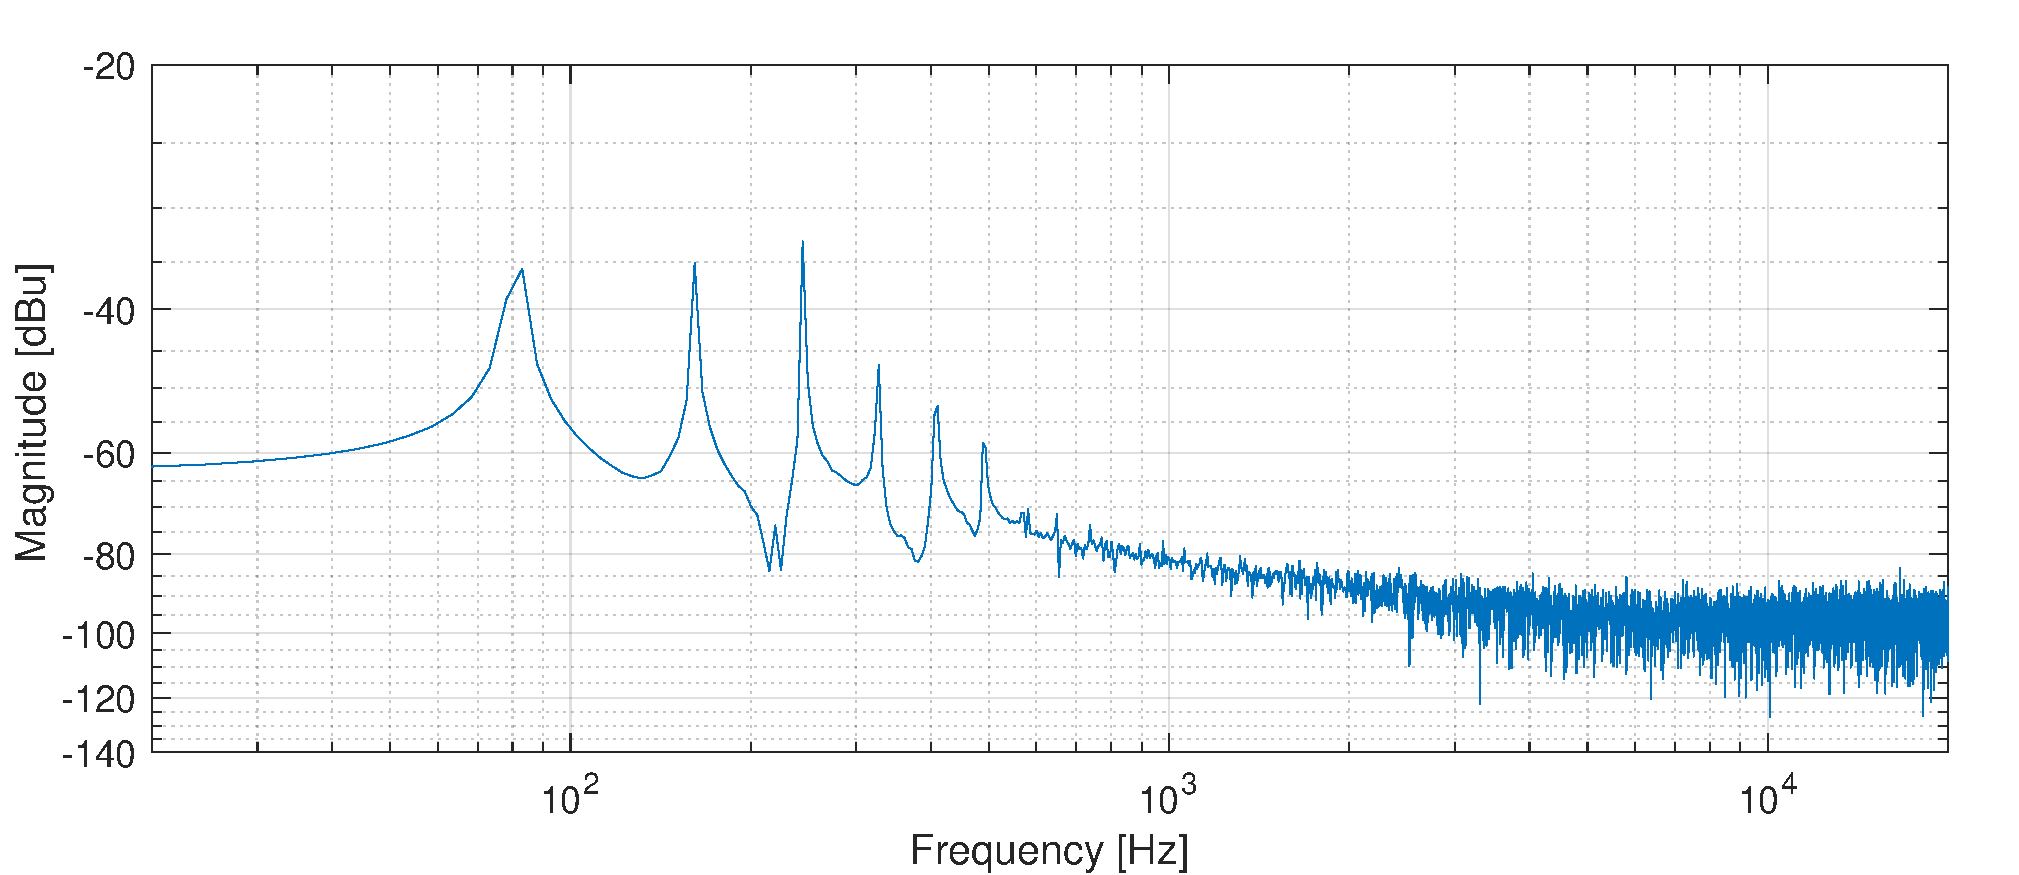
\includegraphics[width=1\textwidth]{guitar_low_E_neck.pdf}
		\caption{Measurement of the low E note on the neck pickup.}
		\label{fig:appendix:low_E_neck}
\end{figure}

On  \autoref{fig:appendix:low_E_neck} it is seen that the lowest significant frequency is around \SI{80}{\hertz} and the highest significant frequency is around \SI{400}{\hertz}, when playing the low E note on the guitar, using the neck pickup.

\begin{figure}[htbp!]
	\centering
		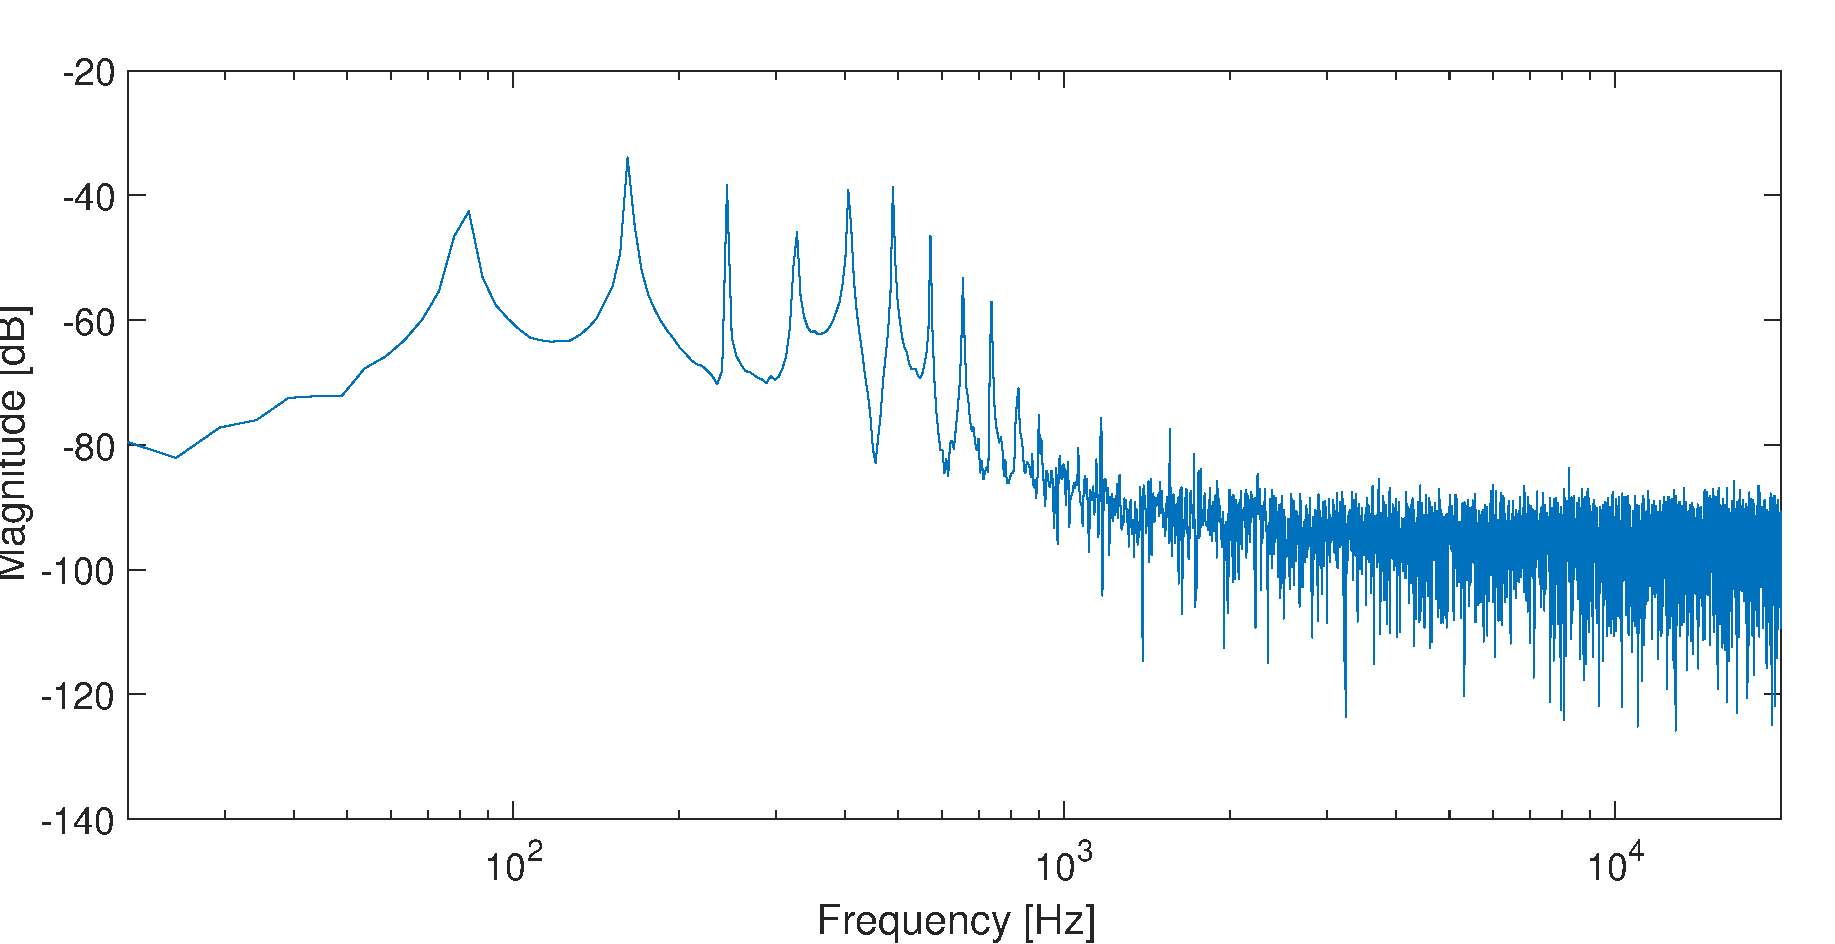
\includegraphics[width=1\textwidth]{guitar_low_E_bridge.pdf}
		\caption{Measurement of the low E note on the bridge pickup.}
		\label{fig:appendix:low_E_bridge}
\end{figure}

On  \autoref{fig:appendix:low_E_bridge} it is seen that the lowest significant frequency is around \SI{80}{\hertz} and the highest significant frequency is around \SI{730}{\hertz}, when playing the low E note on the guitar, using the bridge pickup.

\begin{figure}[htbp!]
	\centering
		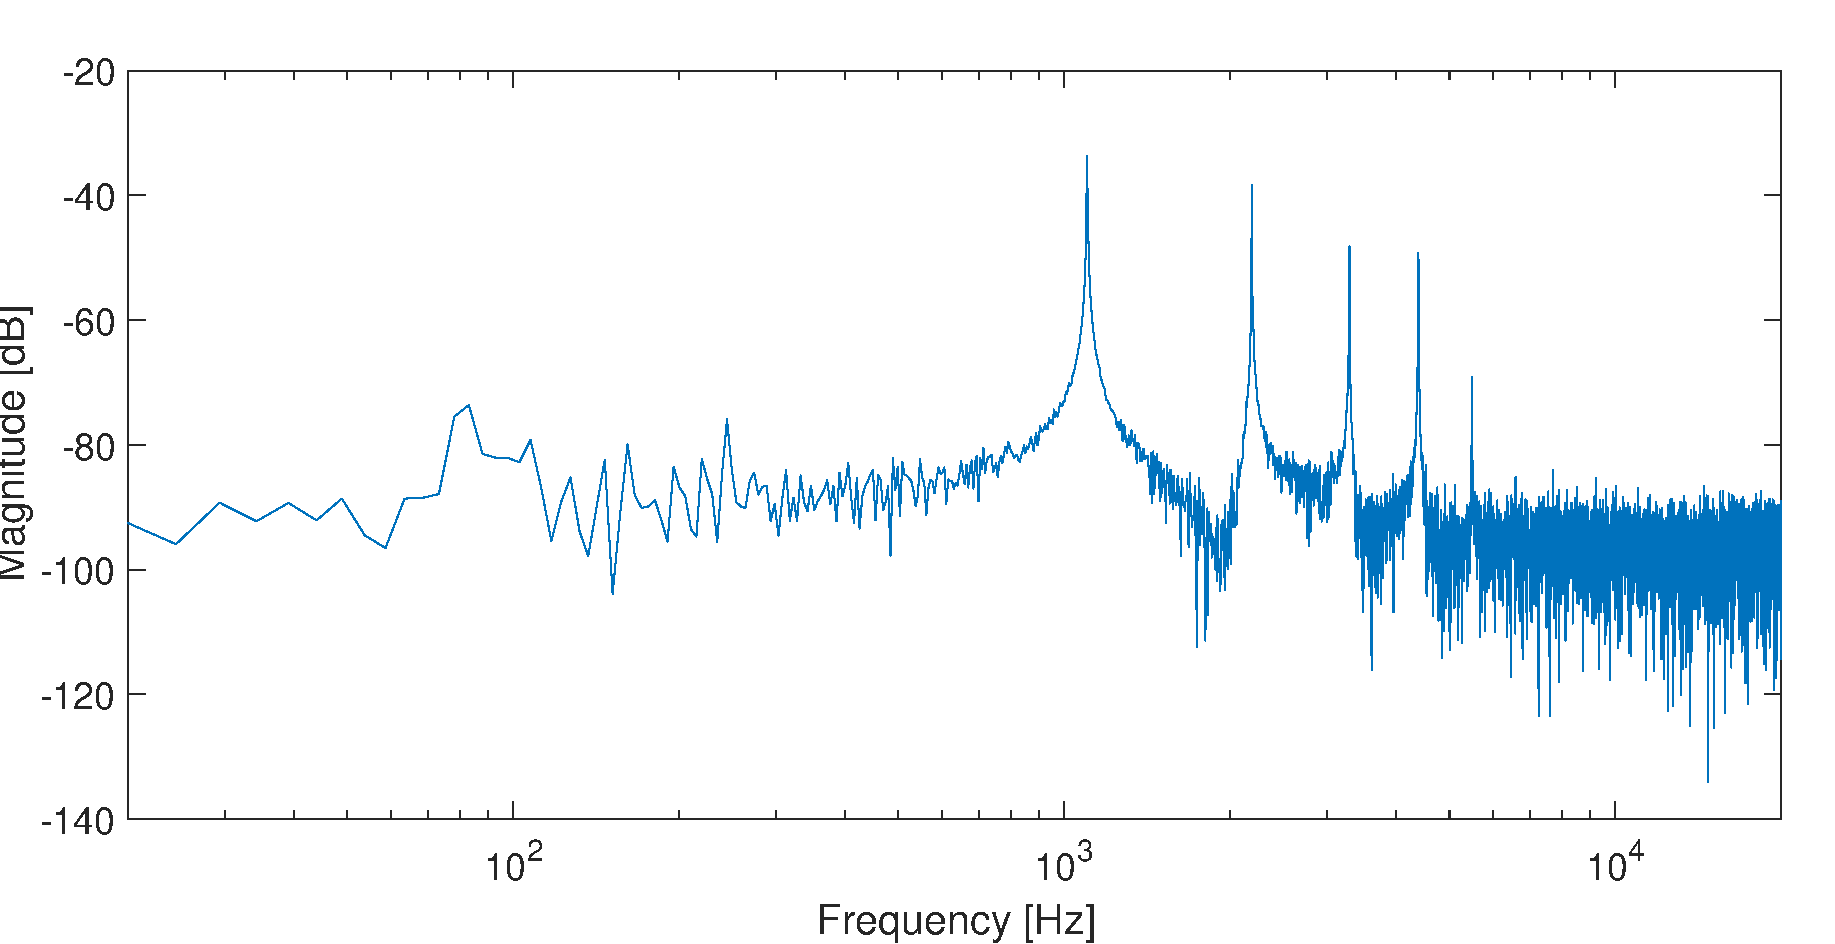
\includegraphics[width=1\textwidth]{guitar_high_Cis_neck.pdf}
		\caption{Measurement of the high C\# note on the neck pickup.}
		\label{fig:appendix:high_Cis_neck}
\end{figure}

On  \autoref{fig:appendix:high_Cis_neck} it is seen that the lowest significant frequency is around \SI{1100}{\hertz} and the highest significant frequency is around \SI{4400}{\hertz}, when playing the high C\# note on the guitar, using the neck pickup.

\begin{figure}[htbp!]
	\centering
		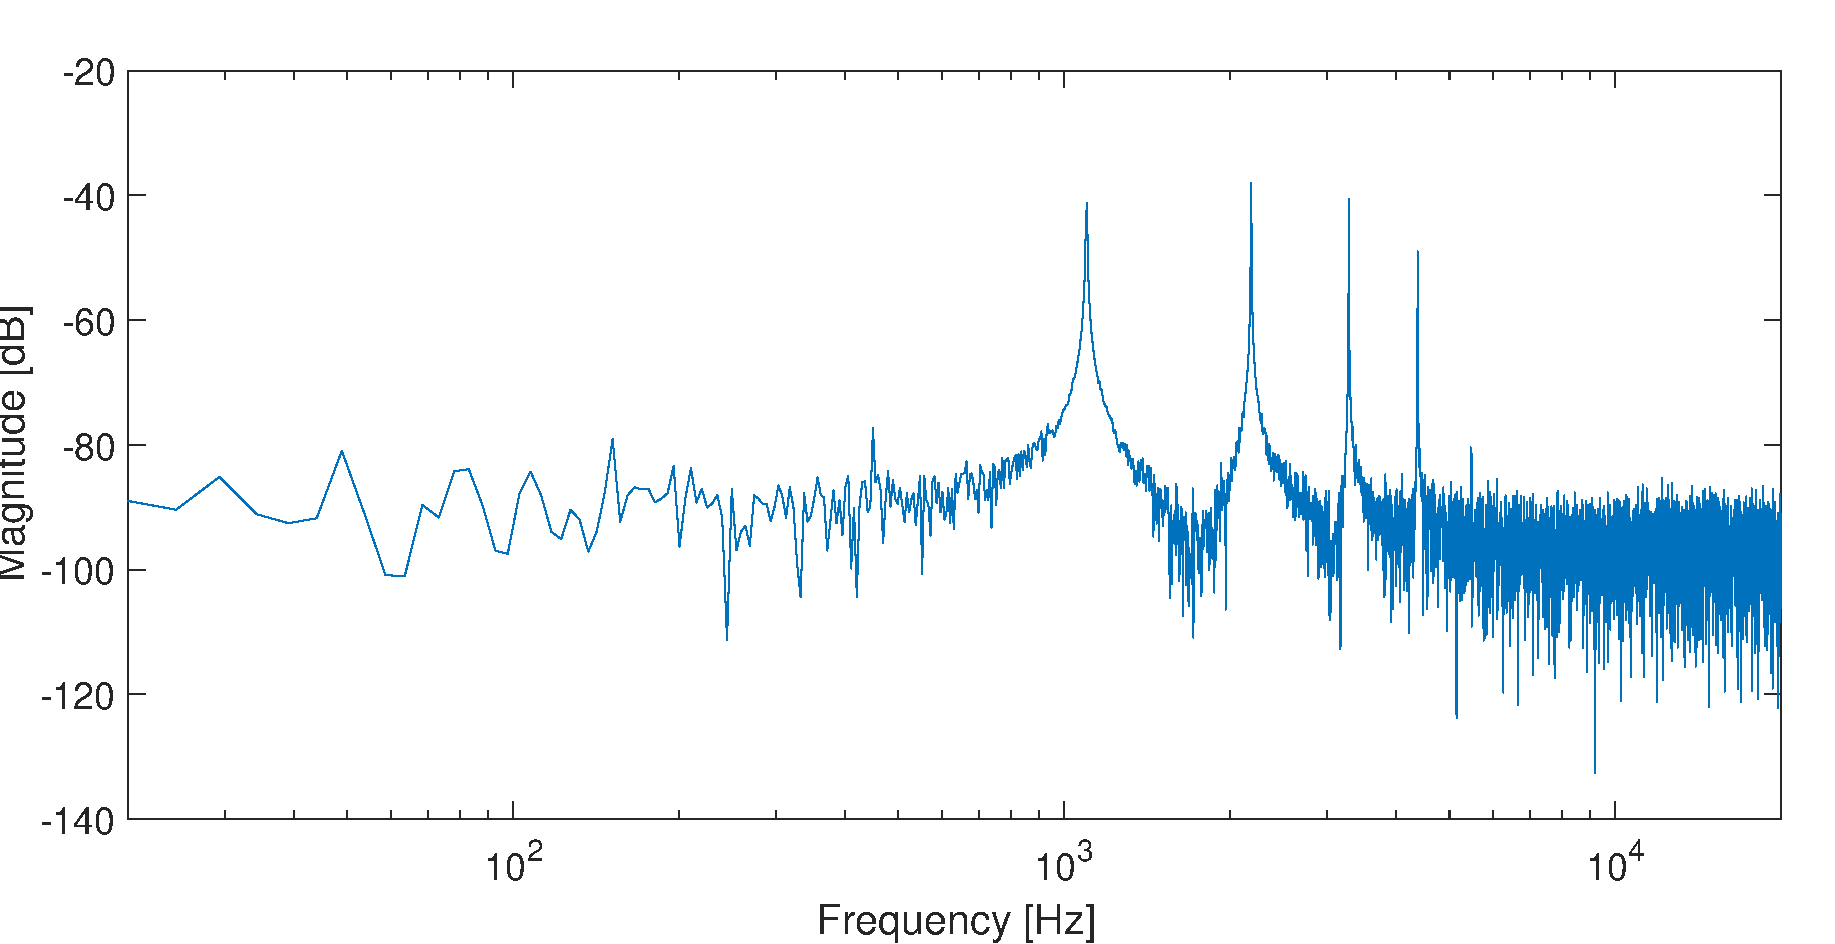
\includegraphics[width=1\textwidth]{guitar_high_Cis_bridge.pdf}
		\caption{Measurement of the high C\# note on the bridge pickup.}
		\label{fig:appendix:high_Cis_bridge}
\end{figure}

On  \autoref{fig:appendix:high_Cis_bridge} it is seen that the lowest significant frequency is around \SI{1100}{\hertz} and the highest significant frequency is around \SI{4400}{\hertz}, when playing the high C\# note on the guitar, using the bridge pickup. 

\begin{figure}[htbp!]
	\centering
		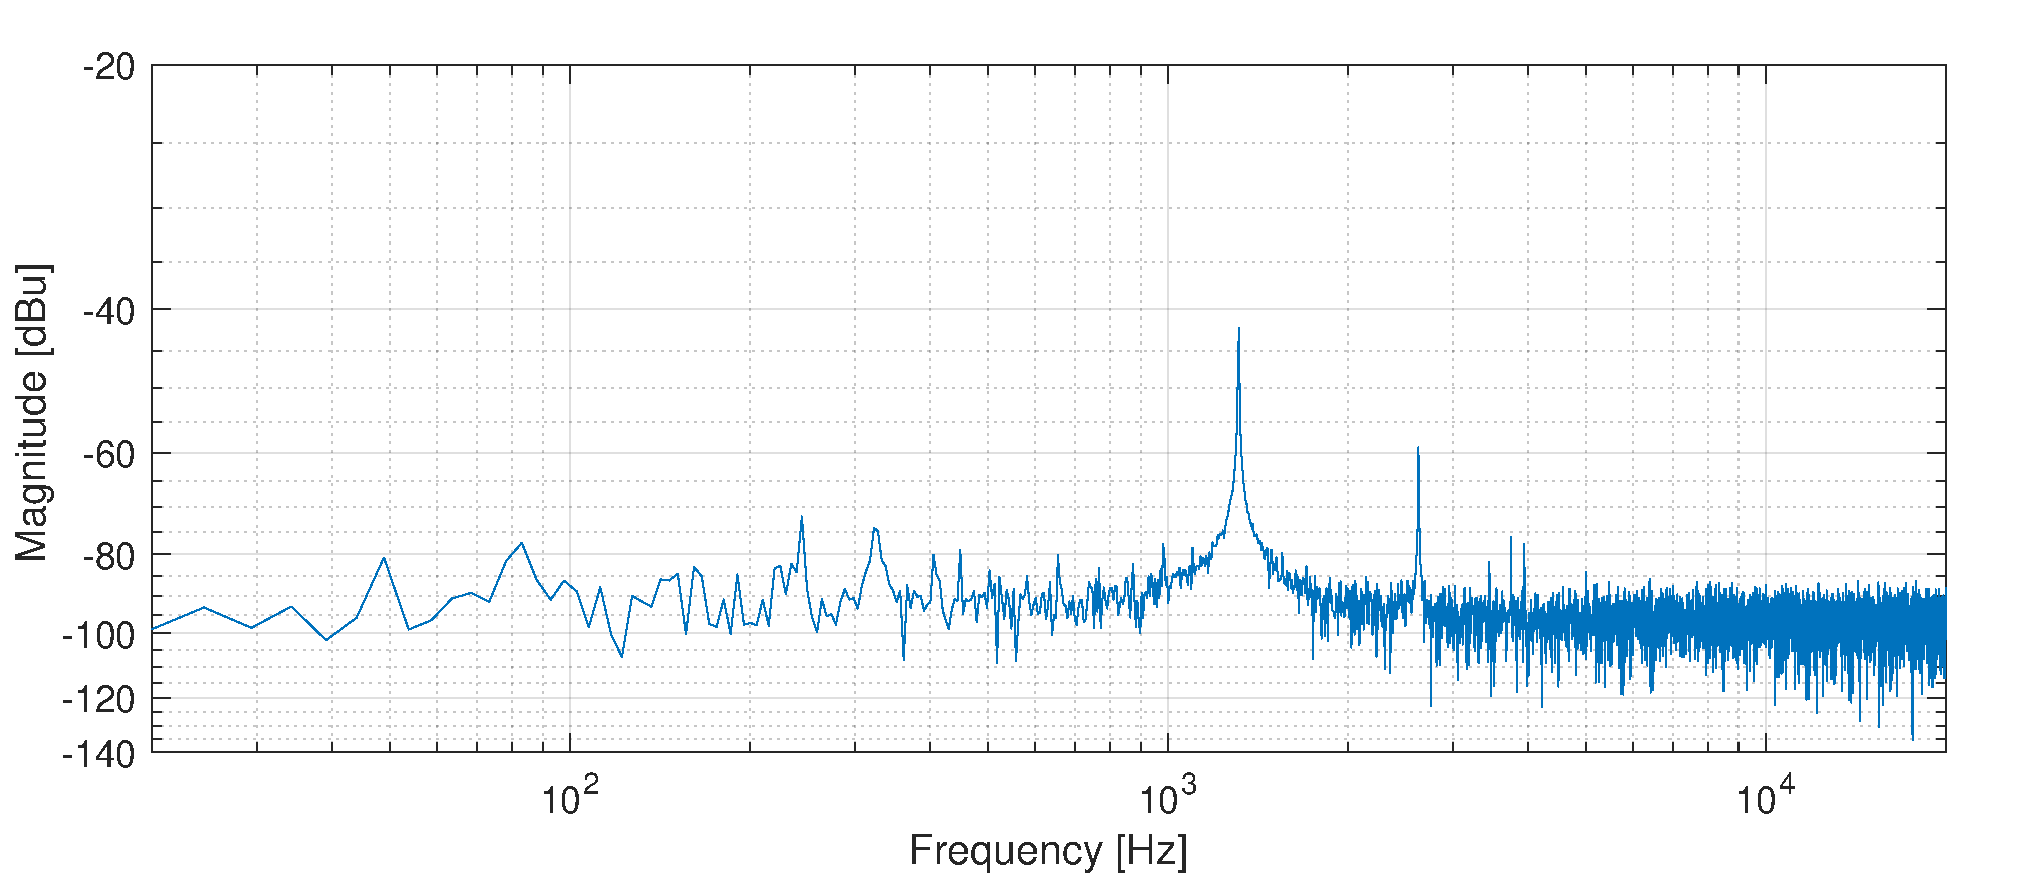
\includegraphics[width=1\textwidth]{guitar_high_E_flasholet_bridge.pdf}
		\caption{Measurement of the high E note, played as flasholet, on the bridge pickup.}
		\label{fig:appendix:high_E_bridge_flasholet}
\end{figure}

On  \autoref{fig:appendix:high_E_bridge_flasholet} it is seen that the lowest significant frequency is around \SI{1300}{\hertz} and the highest significant frequency is around \SI{2600}{\hertz}, when playing the high E note on the guitar as flasholet, using the bridge pickup. 

\chapter{Test a guitars frequency area}\label{app:frequency_area}
A test was made to get a view of the frequency area, in which the tones from a guitar lies.

\section*{Materials and setup}
To measure the frequency area on a guitar, the following materials are used:
\begin{itemize}
\item Digilent Analog Discovery 2 (Oscilloscope)
\item Fender Squier Classic Vibe Telecaster (Guitar)
\item Digilent Waveforms 2015 (PC - software)
\end{itemize}

\begin{figure}[htbp!]
\centering
\def\svgwidth{\columnwidth}
\chapter{Test a guitars frequency area}\label{app:frequency_area}
A test was made to get a view of the frequency area, in which the tones from a guitar lies.

\section*{Materials and setup}
To measure the frequency area on a guitar, the following materials are used:
\begin{itemize}
\item Digilent Analog Discovery 2 (Oscilloscope)
\item Fender Squier Classic Vibe Telecaster (Guitar)
\item Digilent Waveforms 2015 (PC - software)
\end{itemize}

\begin{figure}[htbp!]
\centering
\def\svgwidth{\columnwidth}
\chapter{Test a guitars frequency area}\label{app:frequency_area}
A test was made to get a view of the frequency area, in which the tones from a guitar lies.

\section*{Materials and setup}
To measure the frequency area on a guitar, the following materials are used:
\begin{itemize}
\item Digilent Analog Discovery 2 (Oscilloscope)
\item Fender Squier Classic Vibe Telecaster (Guitar)
\item Digilent Waveforms 2015 (PC - software)
\end{itemize}

\begin{figure}[htbp!]
\centering
\def\svgwidth{\columnwidth}
\input{figures/appendix/guitar_frequency_test.pdf_tex}
\caption{Setup for measuring frequency area on a guitar.}
		\label{fig:appendix:guitar_freq}
\end{figure}

\section*{Test procedure}
To the frequency area on a guitar, the following steps are made:
\begin{enumerate}
\item The materials are set up as in \autoref{fig:appendix:guitar_freq}.
\item Digilent Waveforms 2015 is set as a spectrum analyser. 
\item The guitar is set to use the neck pickup and the volume control and the tone control are turned all the way up.
\item The highest and the lowest tone on the guitar are played, measured by the oscilloscope and analysed in Digilent Waveforms 2015.
\item The guitar is set to use the bridge pickup and step 4 is repeated. 
\item The data is plotted in MATLAB.
\end{enumerate}

\section*{Results}

\begin{figure}[htbp!]
	\centering
		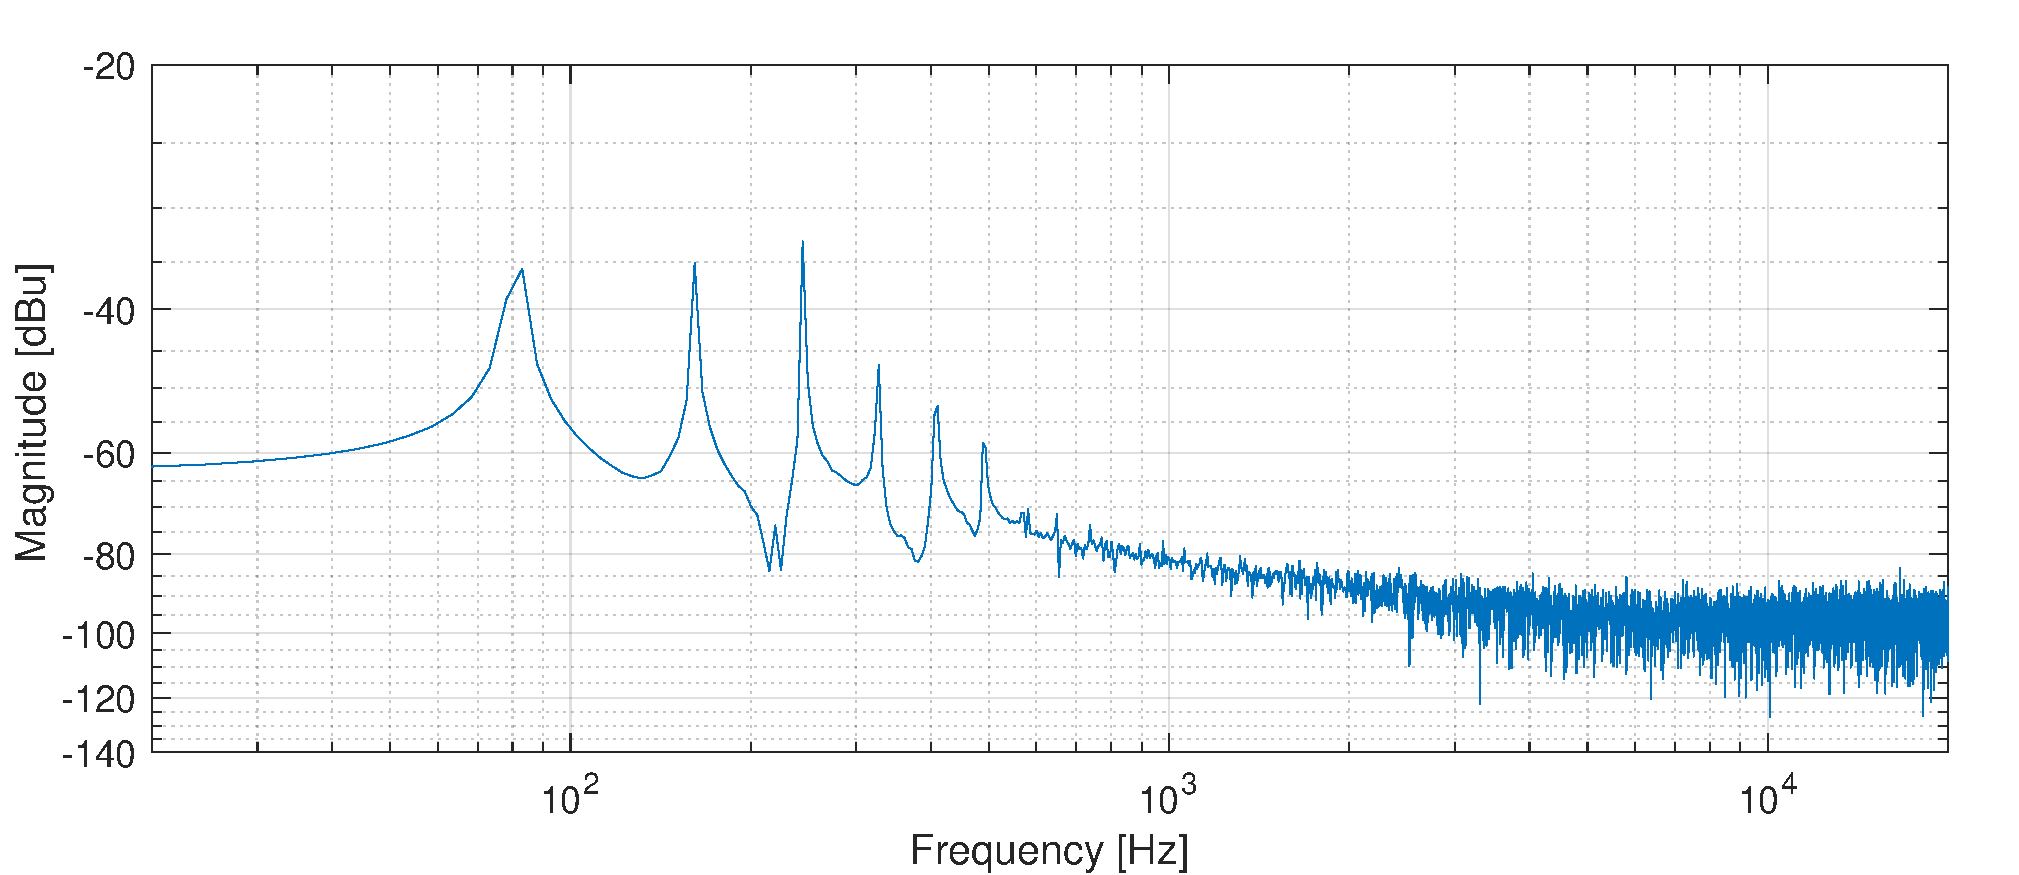
\includegraphics[width=1\textwidth]{guitar_low_E_neck.pdf}
		\caption{Measurement of the low E note on the neck pickup.}
		\label{fig:appendix:low_E_neck}
\end{figure}

On  \autoref{fig:appendix:low_E_neck} it is seen that the lowest significant frequency is around \SI{80}{\hertz} and the highest significant frequency is around \SI{400}{\hertz}, when playing the low E note on the guitar, using the neck pickup.

\begin{figure}[htbp!]
	\centering
		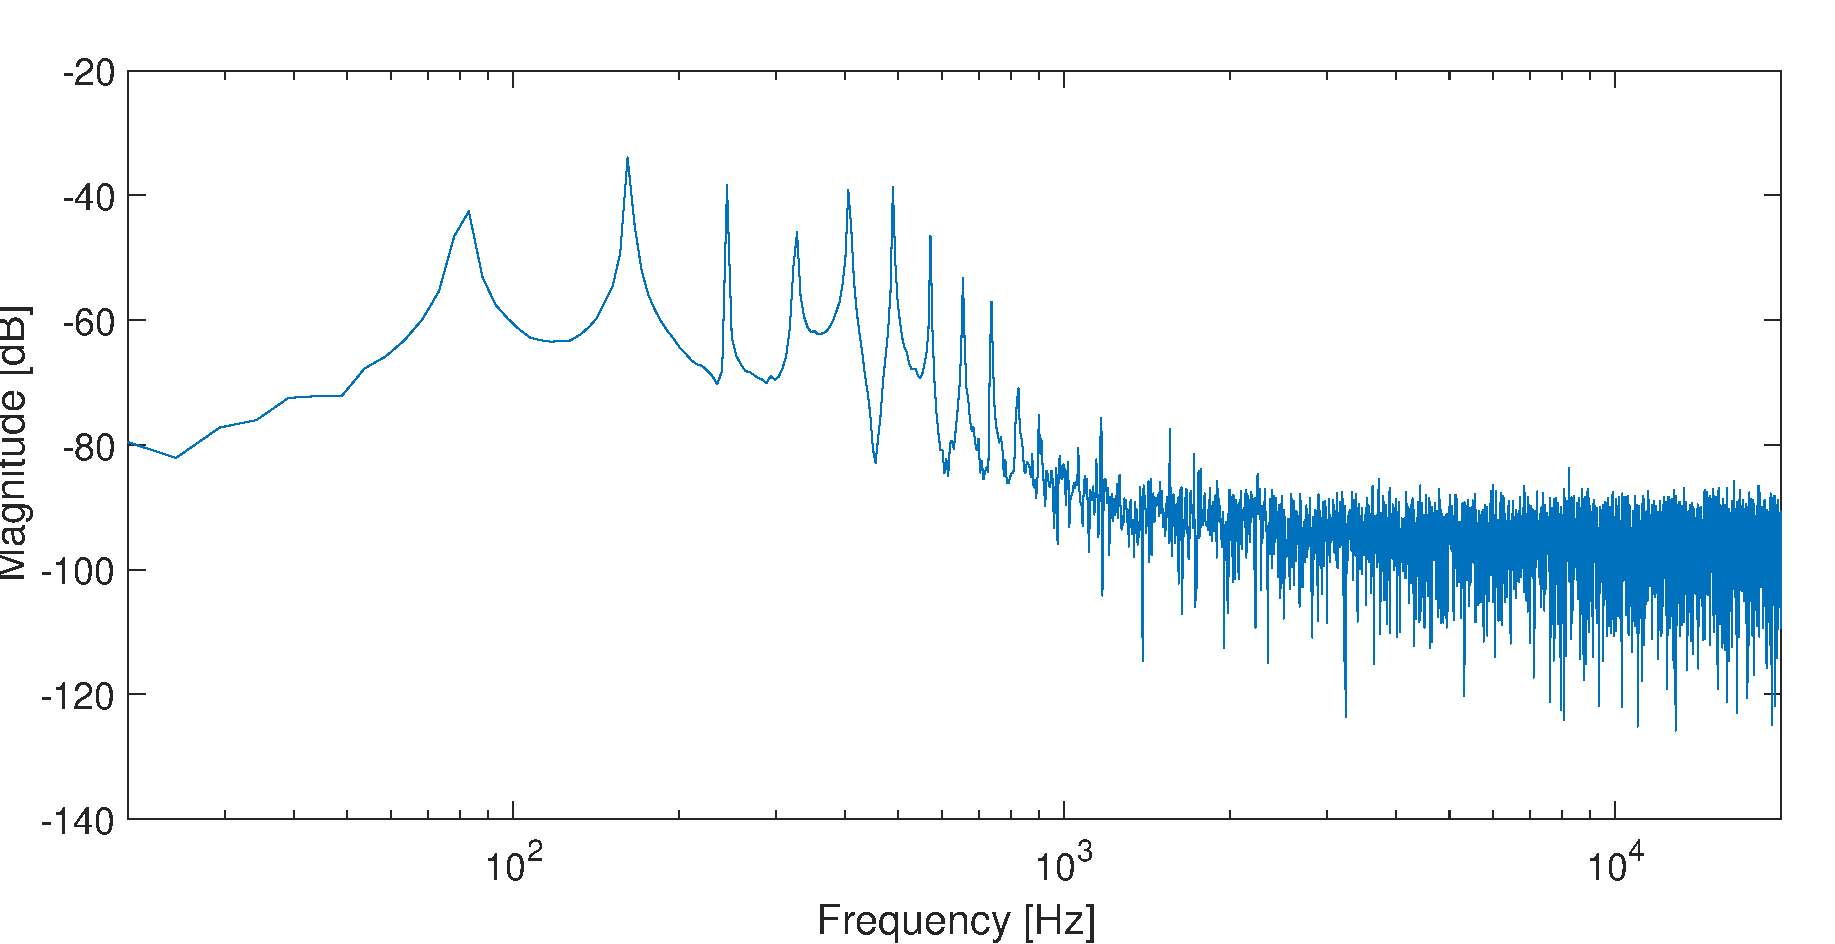
\includegraphics[width=1\textwidth]{guitar_low_E_bridge.pdf}
		\caption{Measurement of the low E note on the bridge pickup.}
		\label{fig:appendix:low_E_bridge}
\end{figure}

On  \autoref{fig:appendix:low_E_bridge} it is seen that the lowest significant frequency is around \SI{80}{\hertz} and the highest significant frequency is around \SI{730}{\hertz}, when playing the low E note on the guitar, using the bridge pickup.

\begin{figure}[htbp!]
	\centering
		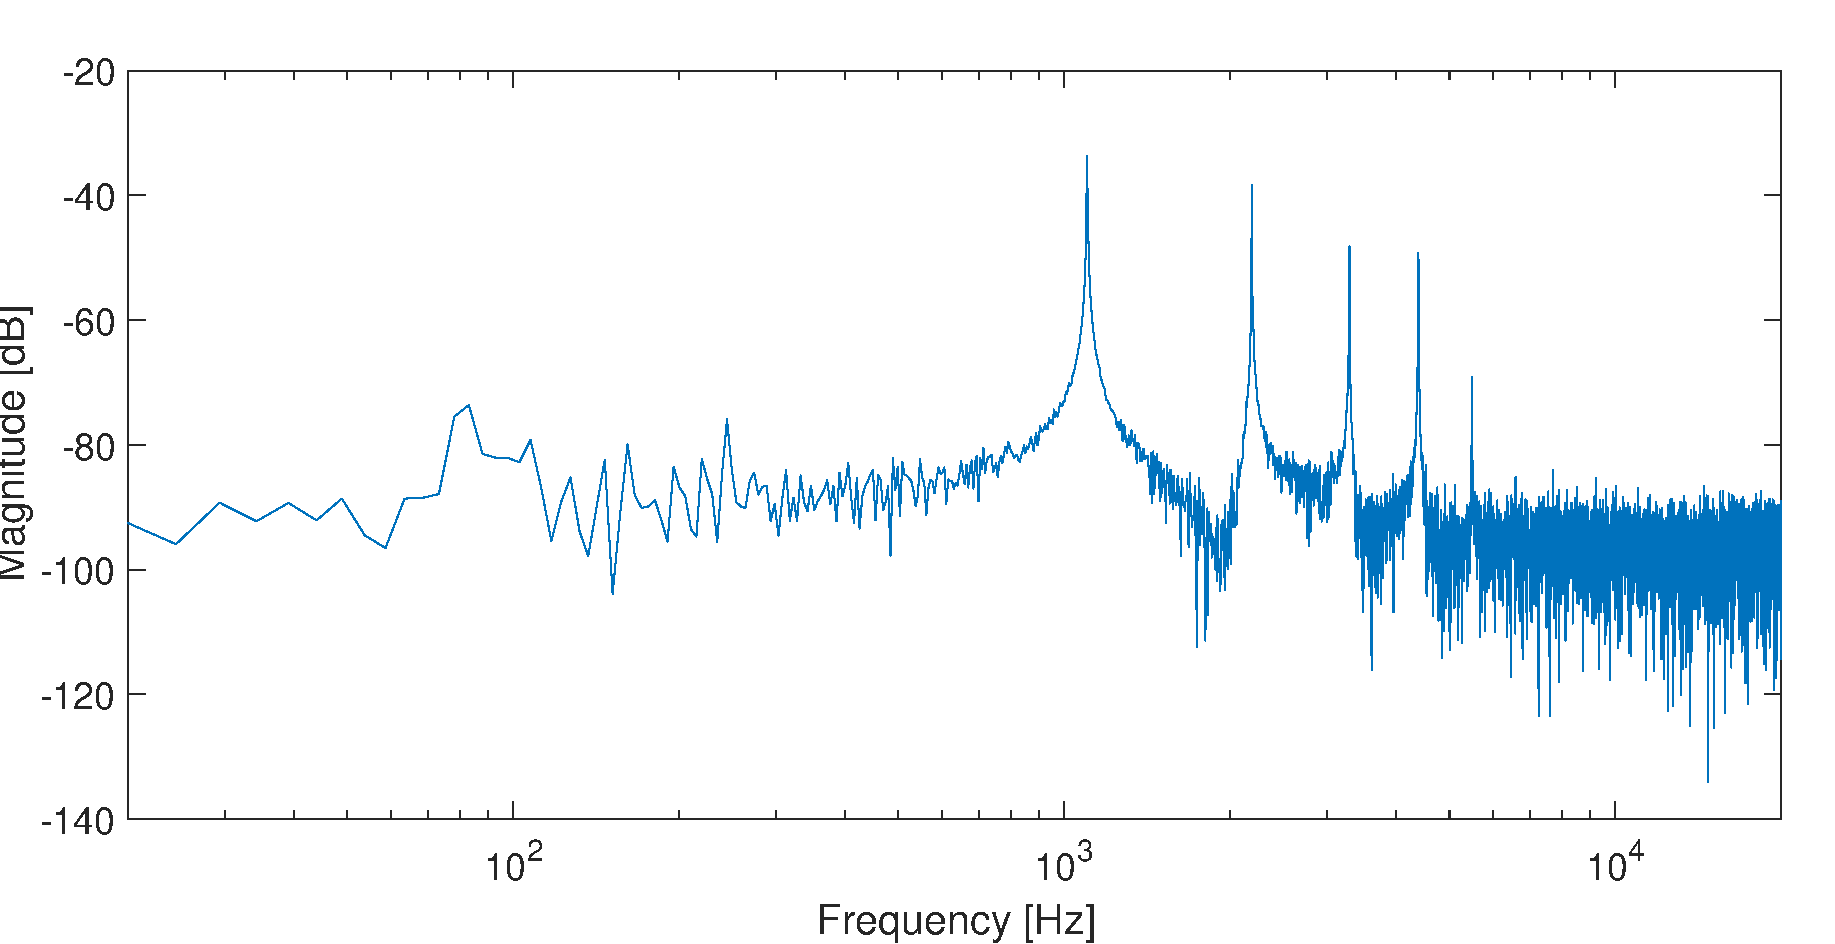
\includegraphics[width=1\textwidth]{guitar_high_Cis_neck.pdf}
		\caption{Measurement of the high C\# note on the neck pickup.}
		\label{fig:appendix:high_Cis_neck}
\end{figure}

On  \autoref{fig:appendix:high_Cis_neck} it is seen that the lowest significant frequency is around \SI{1100}{\hertz} and the highest significant frequency is around \SI{4400}{\hertz}, when playing the high C\# note on the guitar, using the neck pickup.

\begin{figure}[htbp!]
	\centering
		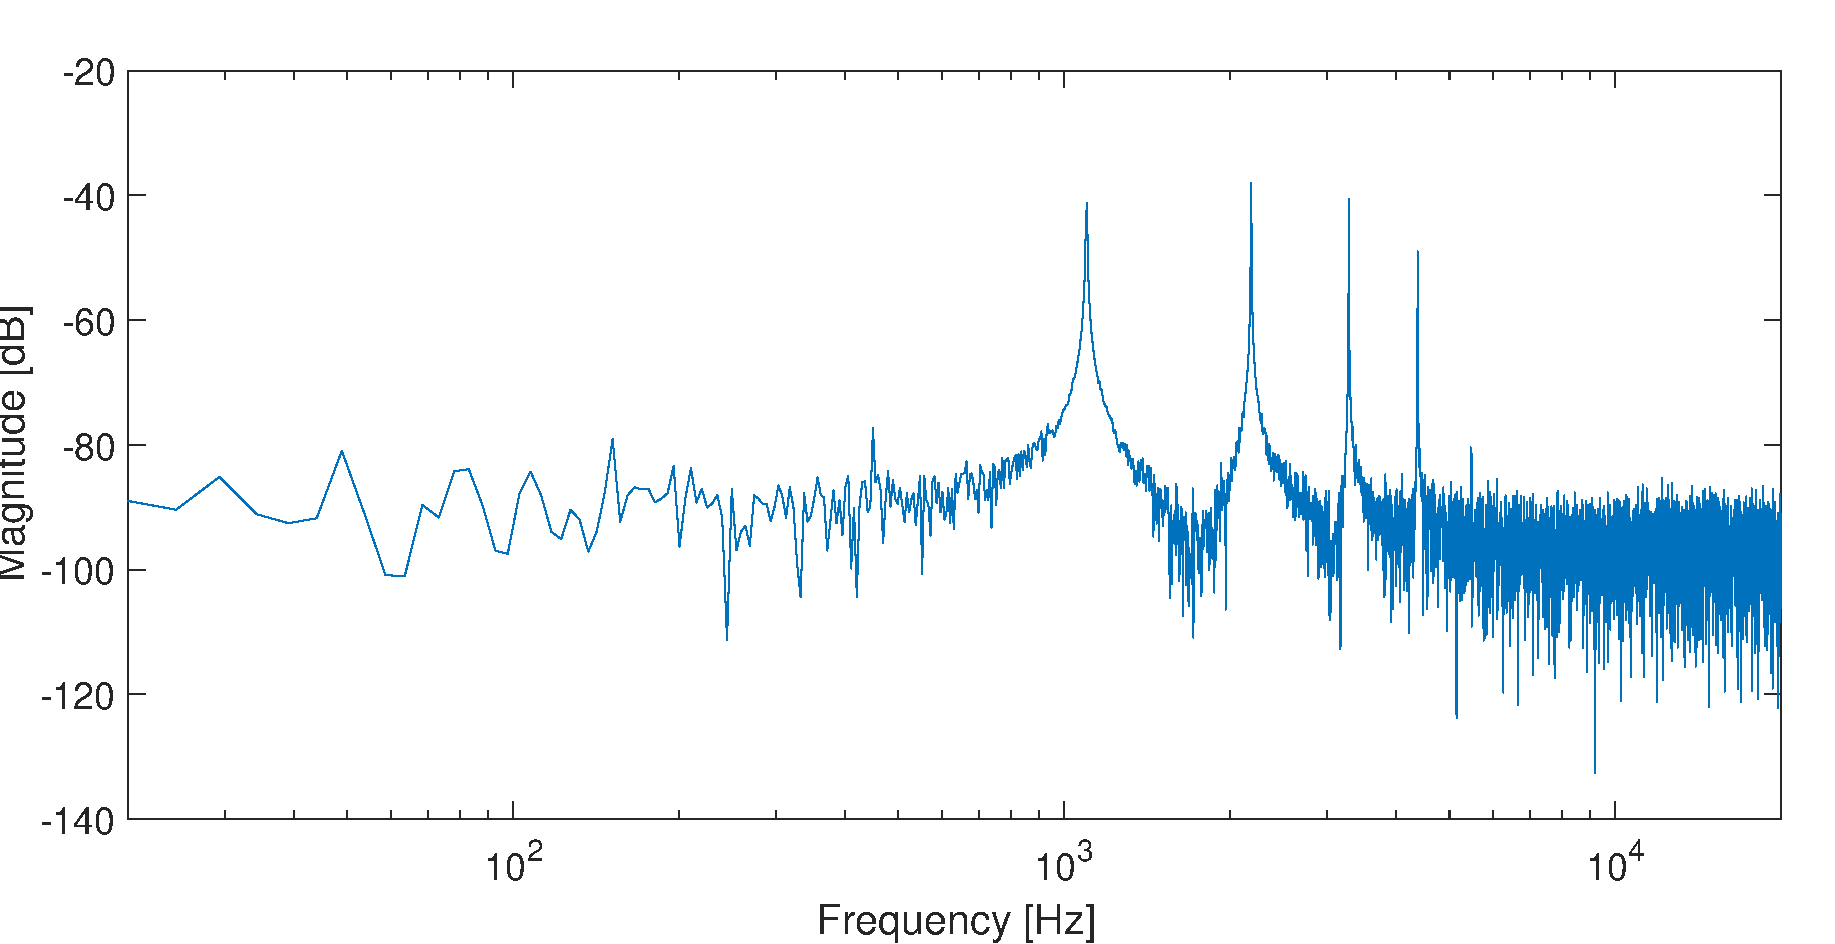
\includegraphics[width=1\textwidth]{guitar_high_Cis_bridge.pdf}
		\caption{Measurement of the high C\# note on the bridge pickup.}
		\label{fig:appendix:high_Cis_bridge}
\end{figure}

On  \autoref{fig:appendix:high_Cis_bridge} it is seen that the lowest significant frequency is around \SI{1100}{\hertz} and the highest significant frequency is around \SI{4400}{\hertz}, when playing the high C\# note on the guitar, using the bridge pickup. 

\begin{figure}[htbp!]
	\centering
		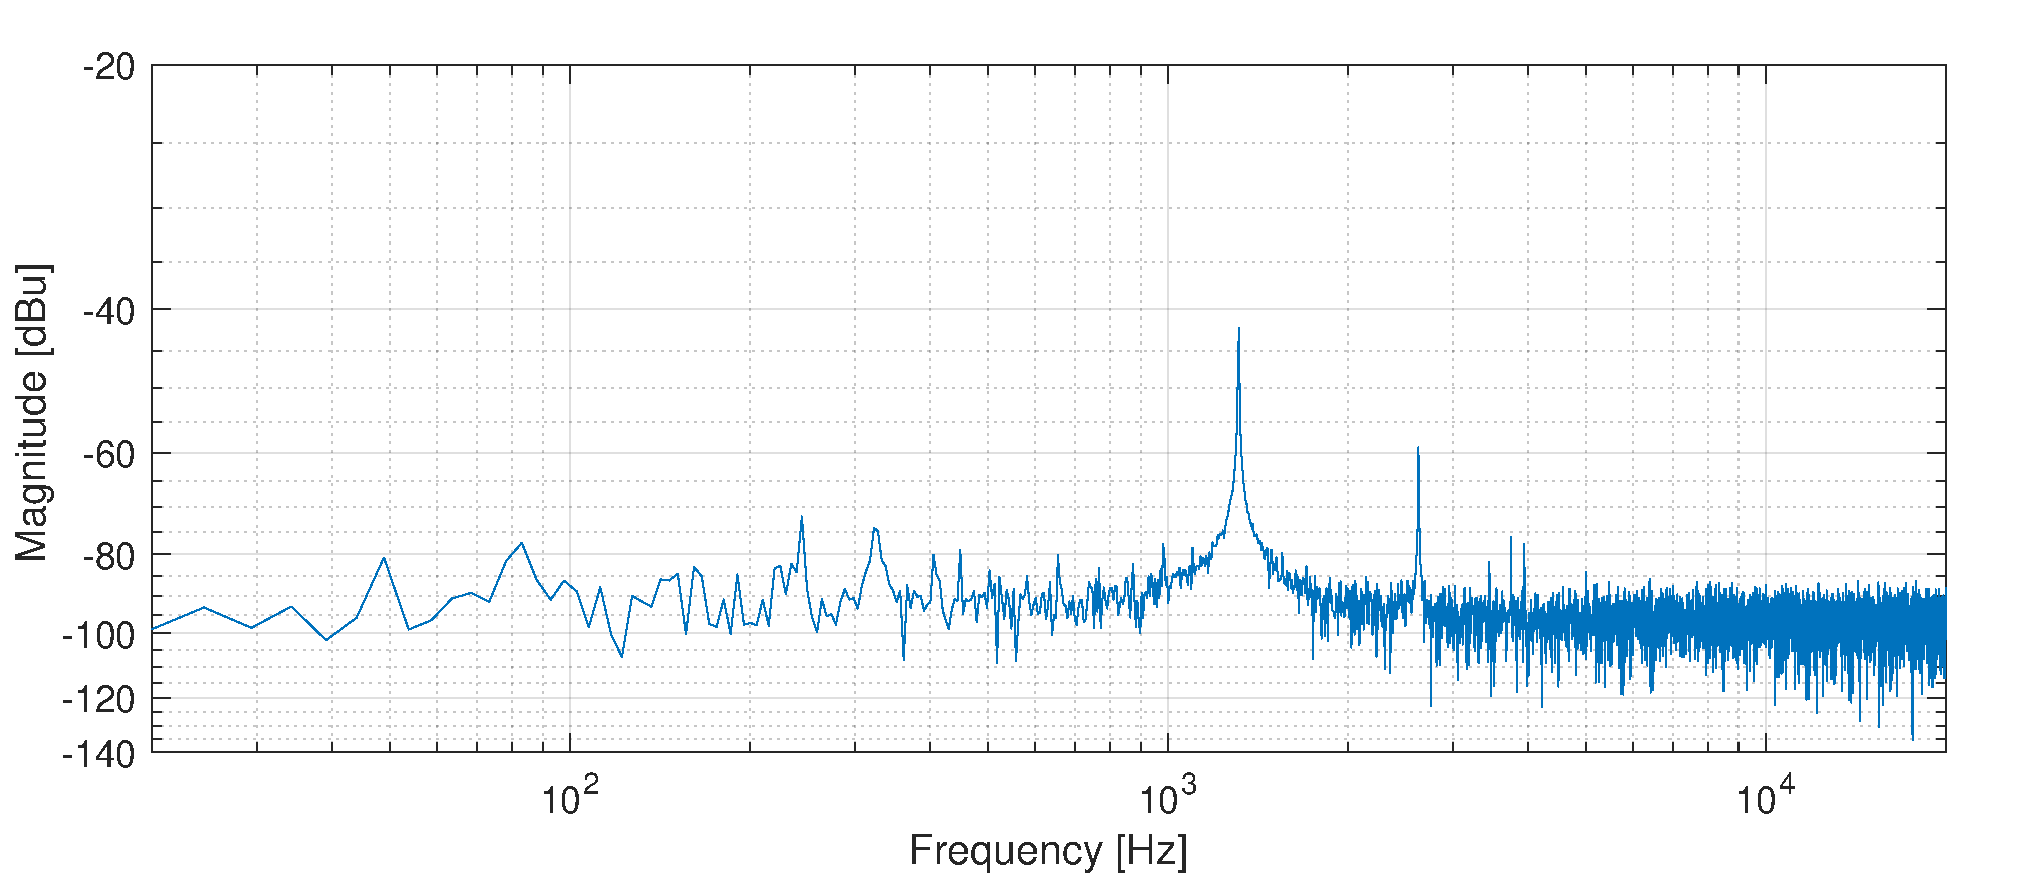
\includegraphics[width=1\textwidth]{guitar_high_E_flasholet_bridge.pdf}
		\caption{Measurement of the high E note, played as flasholet, on the bridge pickup.}
		\label{fig:appendix:high_E_bridge_flasholet}
\end{figure}

On  \autoref{fig:appendix:high_E_bridge_flasholet} it is seen that the lowest significant frequency is around \SI{1300}{\hertz} and the highest significant frequency is around \SI{2600}{\hertz}, when playing the high E note on the guitar as flasholet, using the bridge pickup. 

\caption{Setup for measuring frequency area on a guitar.}
		\label{fig:appendix:guitar_freq}
\end{figure}

\section*{Test procedure}
To the frequency area on a guitar, the following steps are made:
\begin{enumerate}
\item The materials are set up as in \autoref{fig:appendix:guitar_freq}.
\item Digilent Waveforms 2015 is set as a spectrum analyser. 
\item The guitar is set to use the neck pickup and the volume control and the tone control are turned all the way up.
\item The highest and the lowest tone on the guitar are played, measured by the oscilloscope and analysed in Digilent Waveforms 2015.
\item The guitar is set to use the bridge pickup and step 4 is repeated. 
\item The data is plotted in MATLAB.
\end{enumerate}

\section*{Results}

\begin{figure}[htbp!]
	\centering
		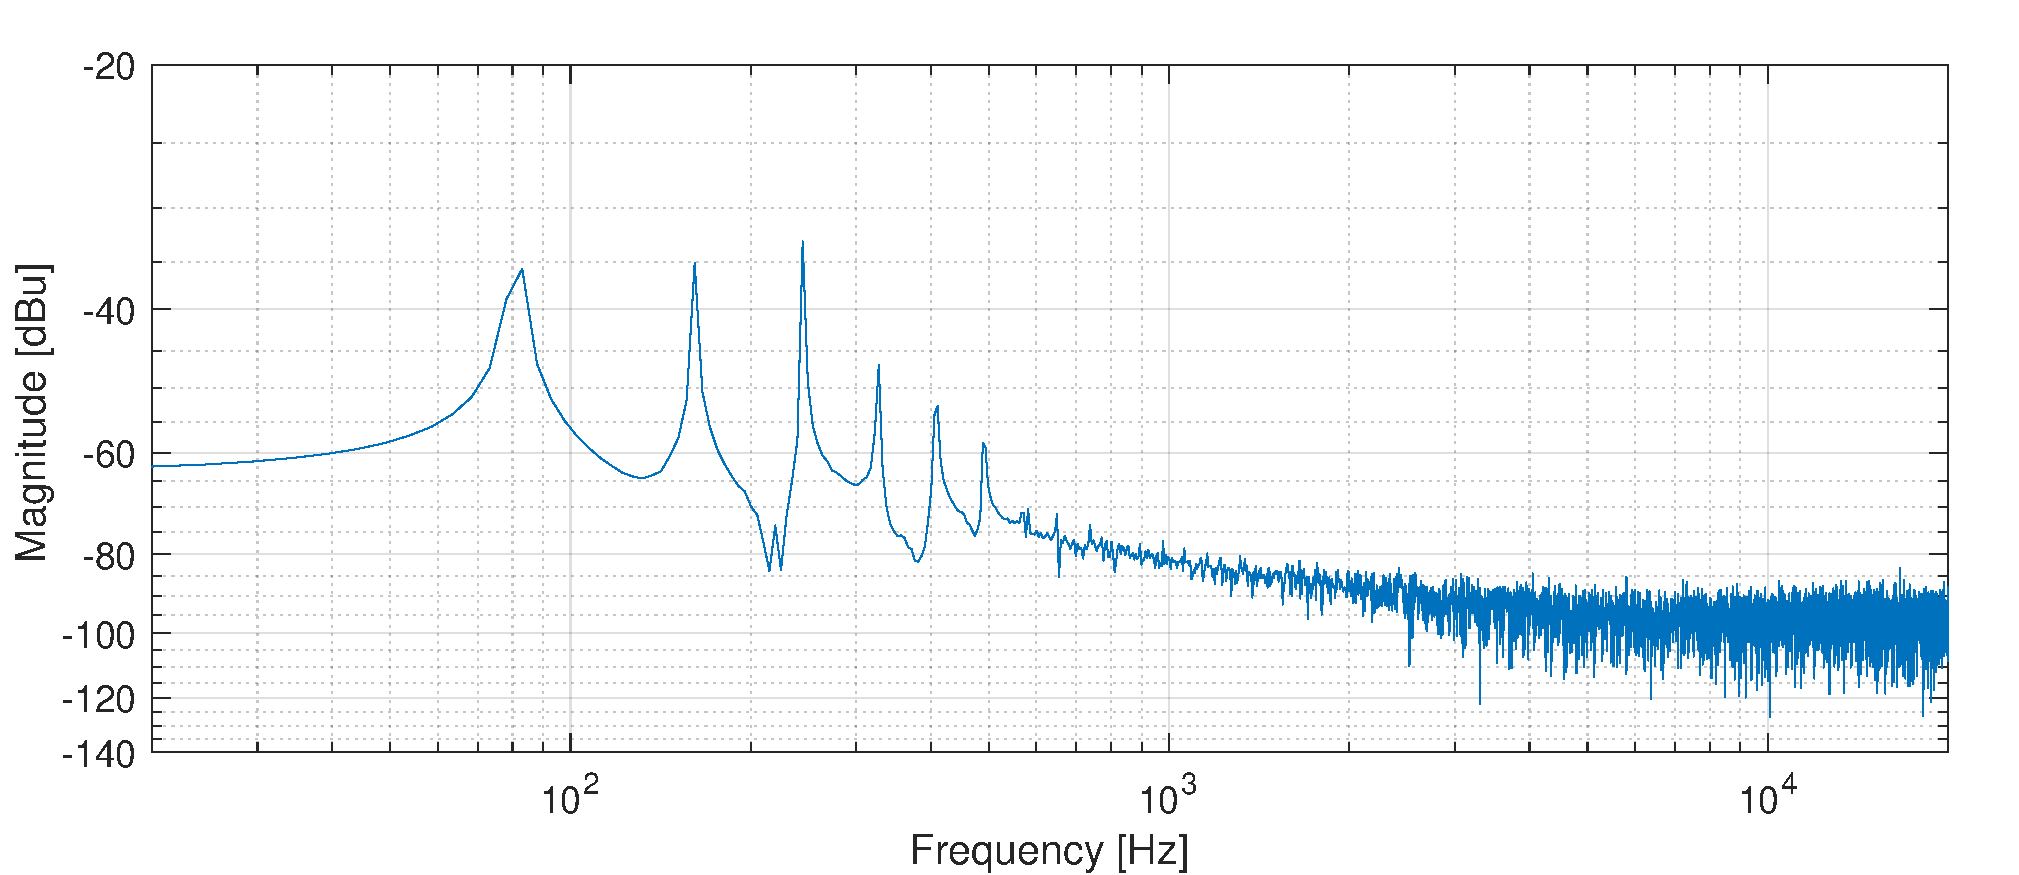
\includegraphics[width=1\textwidth]{guitar_low_E_neck.pdf}
		\caption{Measurement of the low E note on the neck pickup.}
		\label{fig:appendix:low_E_neck}
\end{figure}

On  \autoref{fig:appendix:low_E_neck} it is seen that the lowest significant frequency is around \SI{80}{\hertz} and the highest significant frequency is around \SI{400}{\hertz}, when playing the low E note on the guitar, using the neck pickup.

\begin{figure}[htbp!]
	\centering
		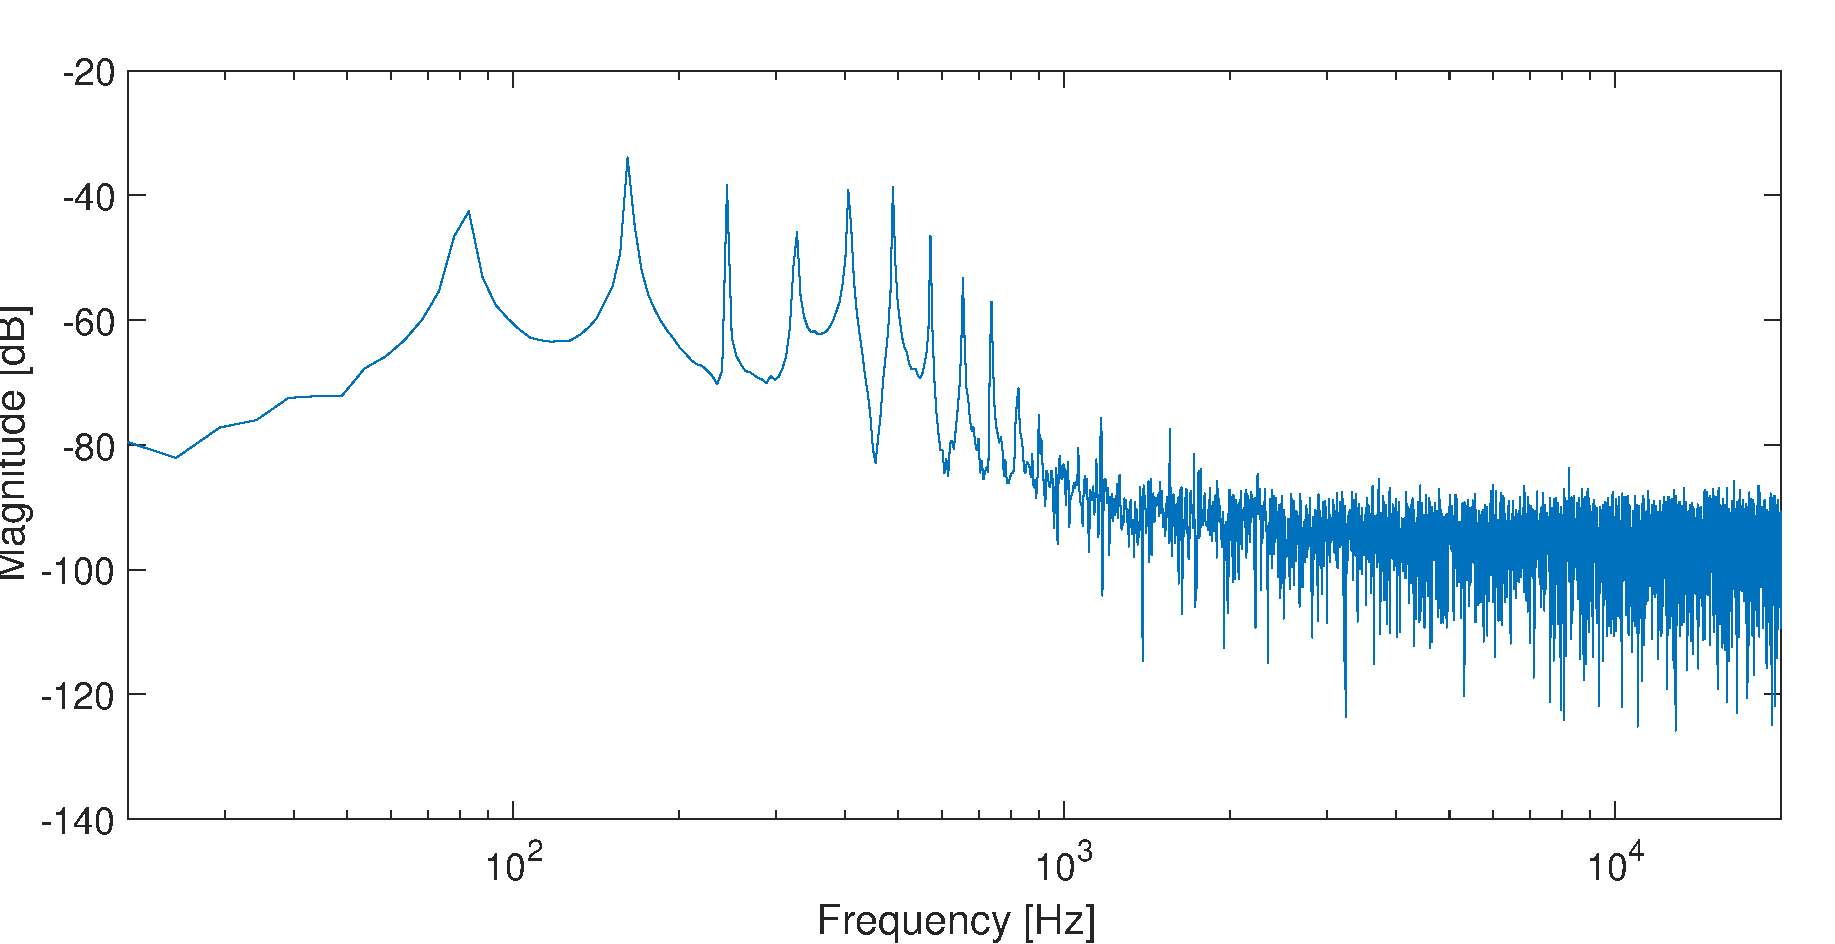
\includegraphics[width=1\textwidth]{guitar_low_E_bridge.pdf}
		\caption{Measurement of the low E note on the bridge pickup.}
		\label{fig:appendix:low_E_bridge}
\end{figure}

On  \autoref{fig:appendix:low_E_bridge} it is seen that the lowest significant frequency is around \SI{80}{\hertz} and the highest significant frequency is around \SI{730}{\hertz}, when playing the low E note on the guitar, using the bridge pickup.

\begin{figure}[htbp!]
	\centering
		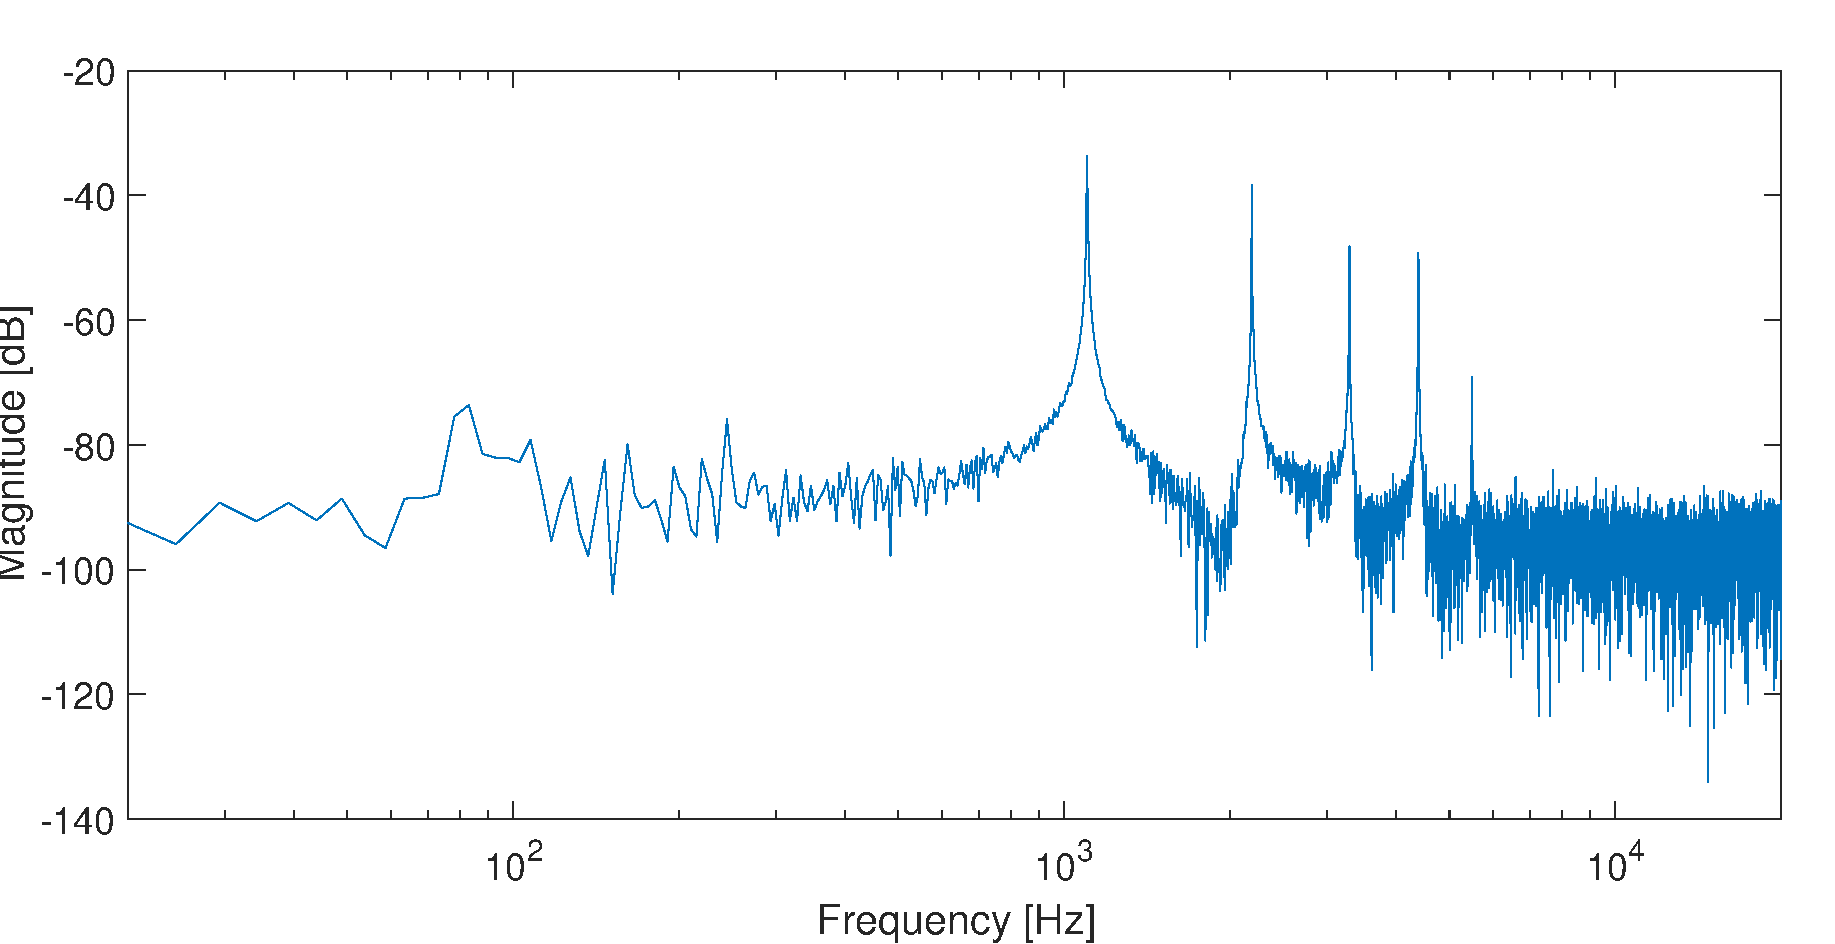
\includegraphics[width=1\textwidth]{guitar_high_Cis_neck.pdf}
		\caption{Measurement of the high C\# note on the neck pickup.}
		\label{fig:appendix:high_Cis_neck}
\end{figure}

On  \autoref{fig:appendix:high_Cis_neck} it is seen that the lowest significant frequency is around \SI{1100}{\hertz} and the highest significant frequency is around \SI{4400}{\hertz}, when playing the high C\# note on the guitar, using the neck pickup.

\begin{figure}[htbp!]
	\centering
		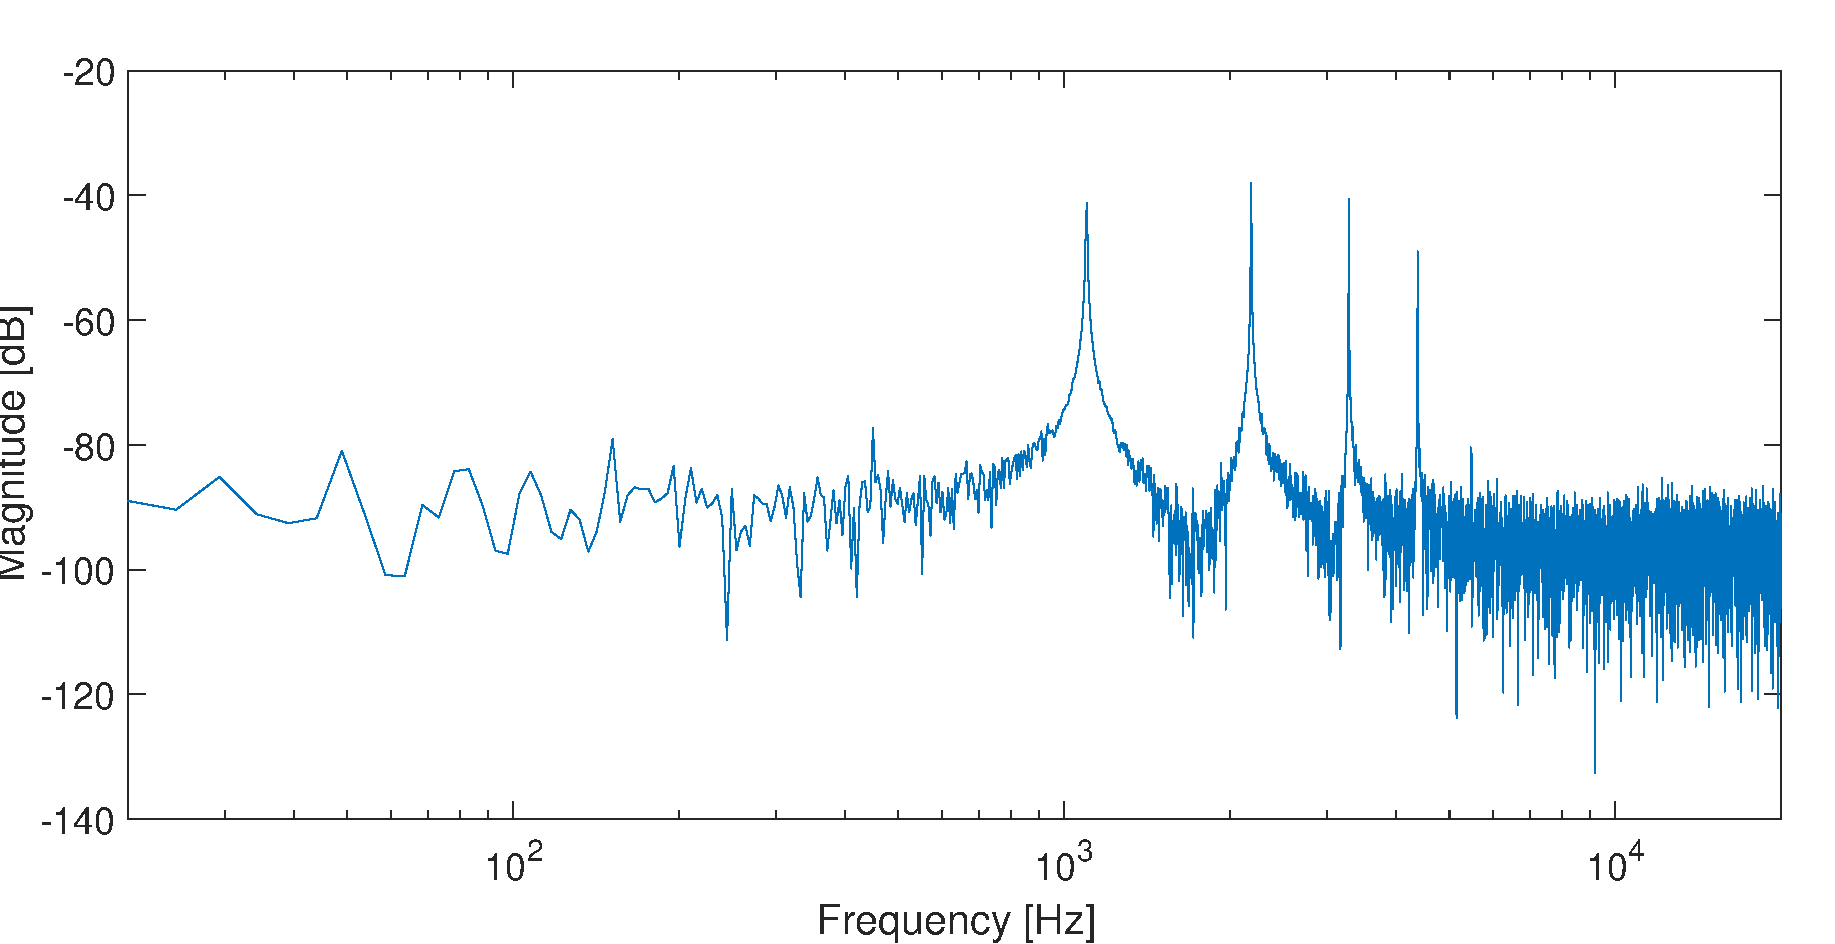
\includegraphics[width=1\textwidth]{guitar_high_Cis_bridge.pdf}
		\caption{Measurement of the high C\# note on the bridge pickup.}
		\label{fig:appendix:high_Cis_bridge}
\end{figure}

On  \autoref{fig:appendix:high_Cis_bridge} it is seen that the lowest significant frequency is around \SI{1100}{\hertz} and the highest significant frequency is around \SI{4400}{\hertz}, when playing the high C\# note on the guitar, using the bridge pickup. 

\begin{figure}[htbp!]
	\centering
		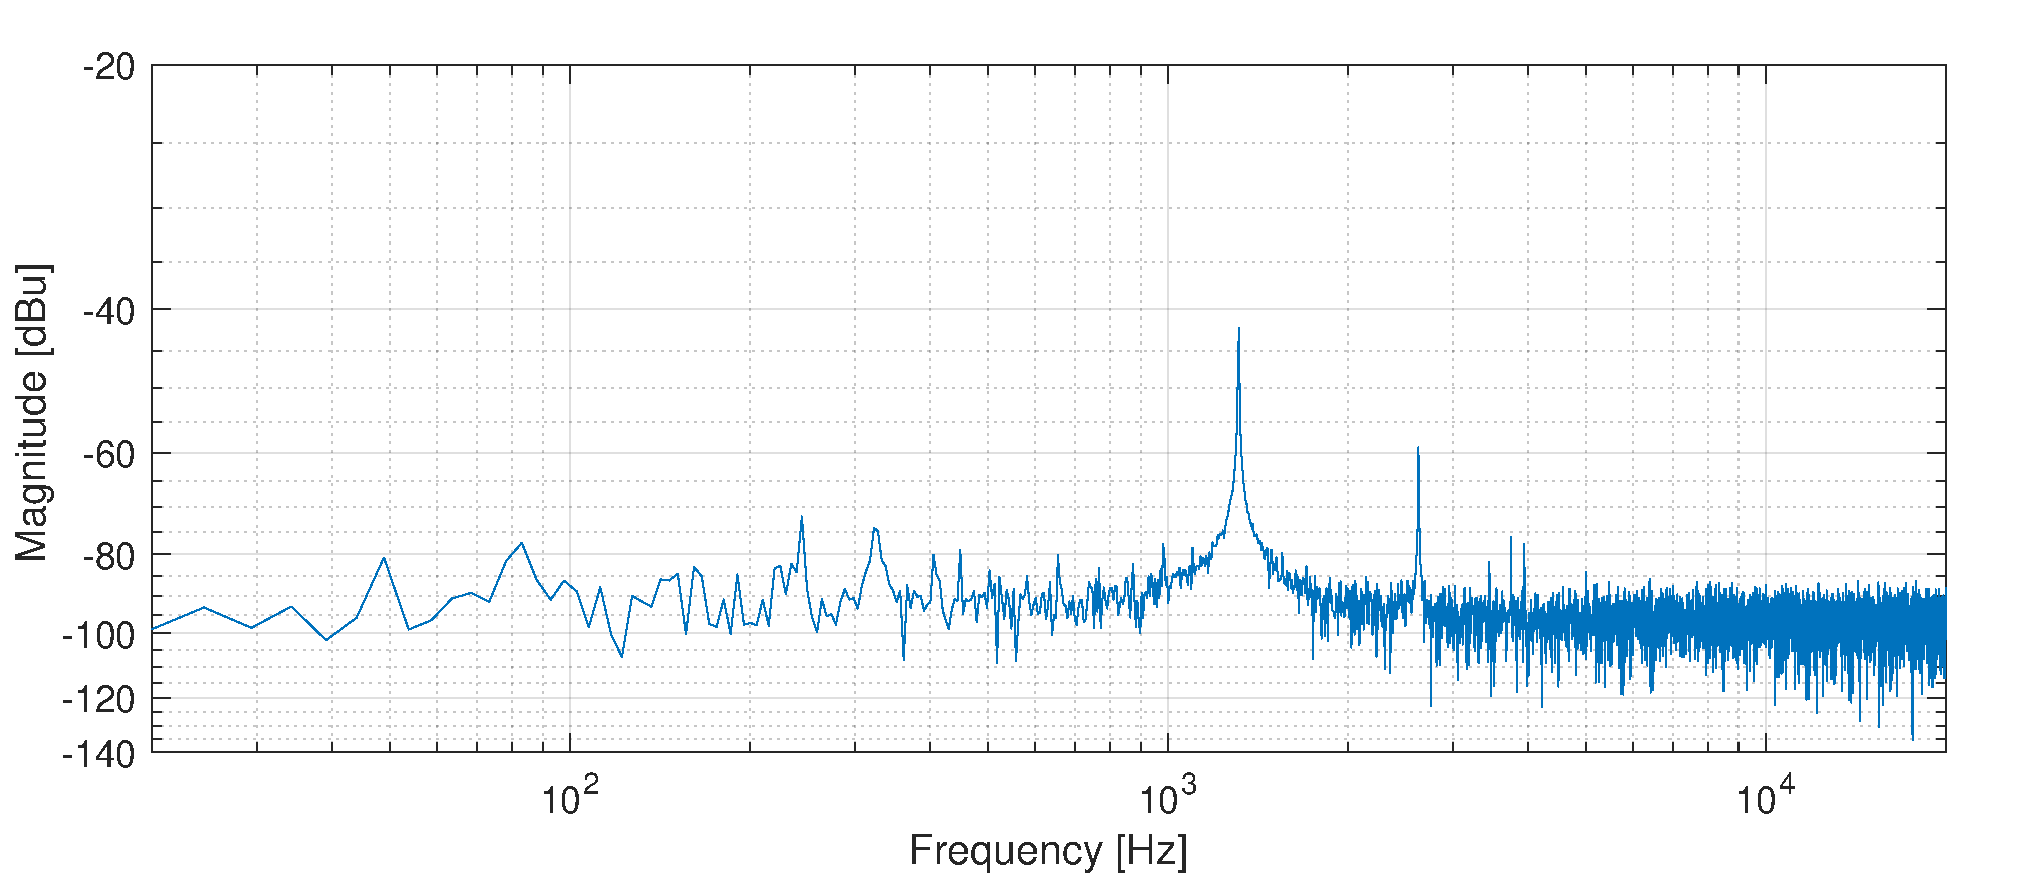
\includegraphics[width=1\textwidth]{guitar_high_E_flasholet_bridge.pdf}
		\caption{Measurement of the high E note, played as flasholet, on the bridge pickup.}
		\label{fig:appendix:high_E_bridge_flasholet}
\end{figure}

On  \autoref{fig:appendix:high_E_bridge_flasholet} it is seen that the lowest significant frequency is around \SI{1300}{\hertz} and the highest significant frequency is around \SI{2600}{\hertz}, when playing the high E note on the guitar as flasholet, using the bridge pickup. 

\caption{Setup for measuring frequency area on a guitar.}
		\label{fig:appendix:guitar_freq}
\end{figure}

\section*{Test procedure}
To the frequency area on a guitar, the following steps are made:
\begin{enumerate}
\item The materials are set up as in \autoref{fig:appendix:guitar_freq}.
\item Digilent Waveforms 2015 is set as a spectrum analyser. 
\item The guitar is set to use the neck pickup and the volume control and the tone control are turned all the way up.
\item The highest and the lowest tone on the guitar are played, measured by the oscilloscope and analysed in Digilent Waveforms 2015.
\item The guitar is set to use the bridge pickup and step 4 is repeated. 
\item The data is plotted in MATLAB.
\end{enumerate}

\section*{Results}

\begin{figure}[htbp!]
	\centering
		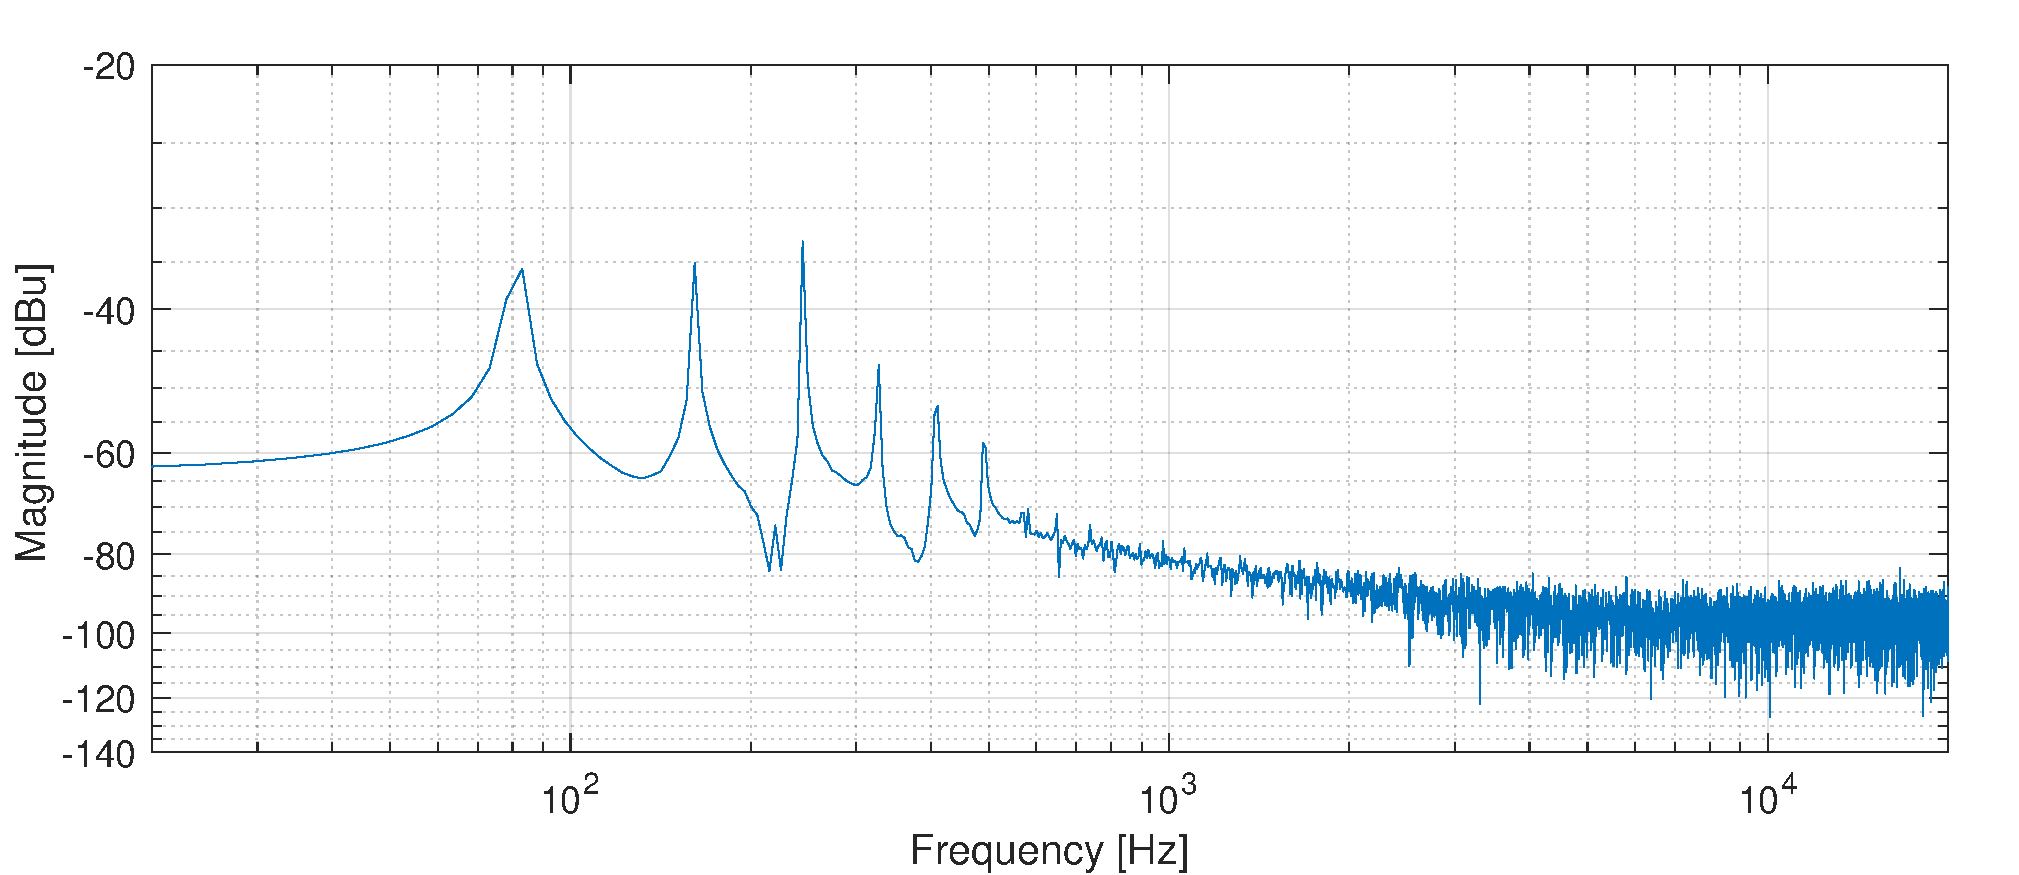
\includegraphics[width=1\textwidth]{guitar_low_E_neck.pdf}
		\caption{Measurement of the low E note on the neck pickup.}
		\label{fig:appendix:low_E_neck}
\end{figure}

On  \autoref{fig:appendix:low_E_neck} it is seen that the lowest significant frequency is around \SI{80}{\hertz} and the highest significant frequency is around \SI{400}{\hertz}, when playing the low E note on the guitar, using the neck pickup.

\begin{figure}[htbp!]
	\centering
		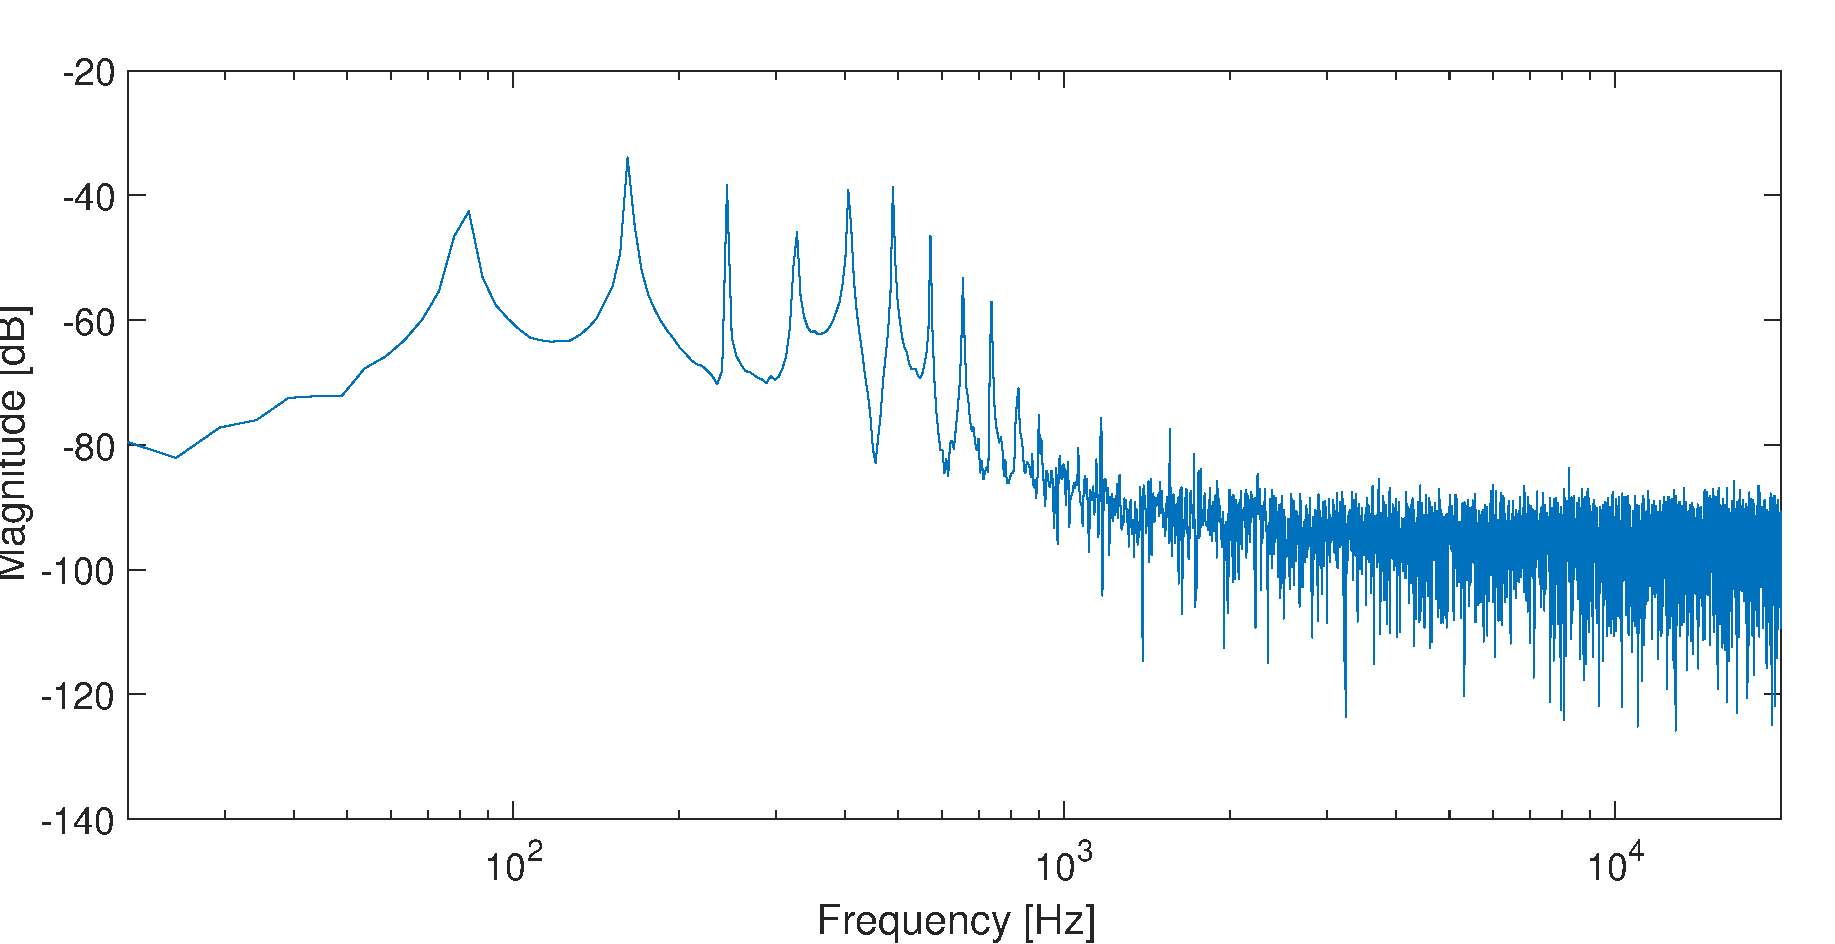
\includegraphics[width=1\textwidth]{guitar_low_E_bridge.pdf}
		\caption{Measurement of the low E note on the bridge pickup.}
		\label{fig:appendix:low_E_bridge}
\end{figure}

On  \autoref{fig:appendix:low_E_bridge} it is seen that the lowest significant frequency is around \SI{80}{\hertz} and the highest significant frequency is around \SI{730}{\hertz}, when playing the low E note on the guitar, using the bridge pickup.

\begin{figure}[htbp!]
	\centering
		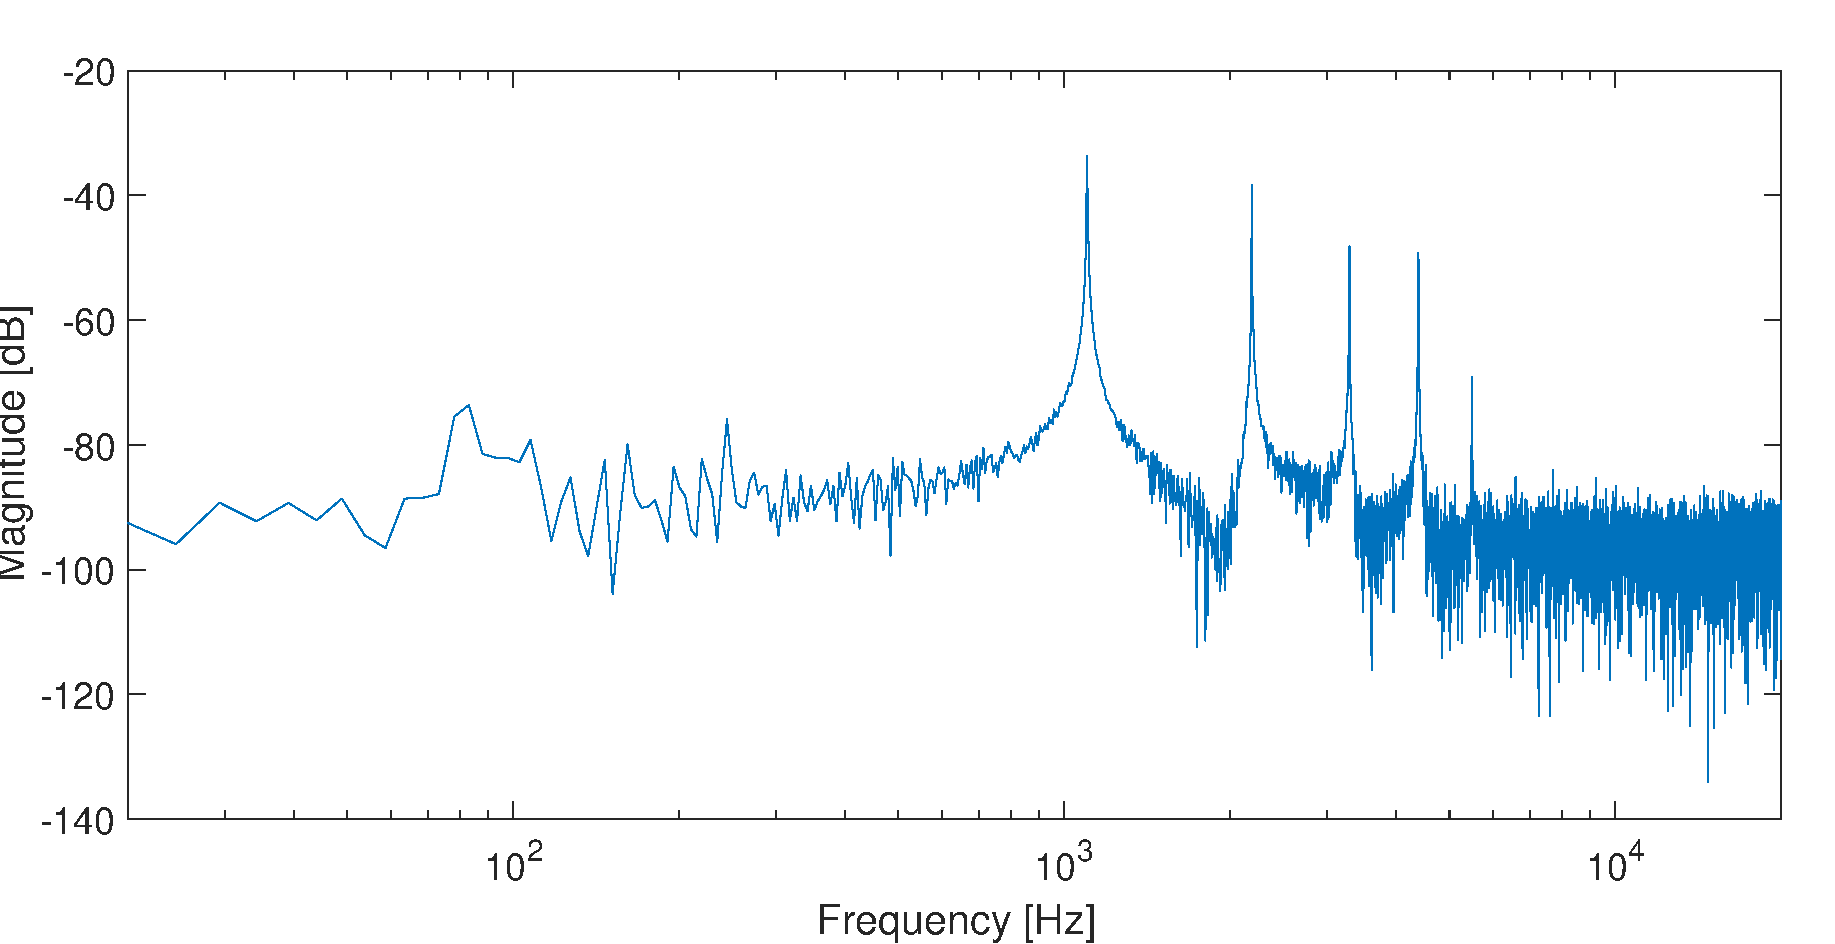
\includegraphics[width=1\textwidth]{guitar_high_Cis_neck.pdf}
		\caption{Measurement of the high C\# note on the neck pickup.}
		\label{fig:appendix:high_Cis_neck}
\end{figure}

On  \autoref{fig:appendix:high_Cis_neck} it is seen that the lowest significant frequency is around \SI{1100}{\hertz} and the highest significant frequency is around \SI{4400}{\hertz}, when playing the high C\# note on the guitar, using the neck pickup.

\begin{figure}[htbp!]
	\centering
		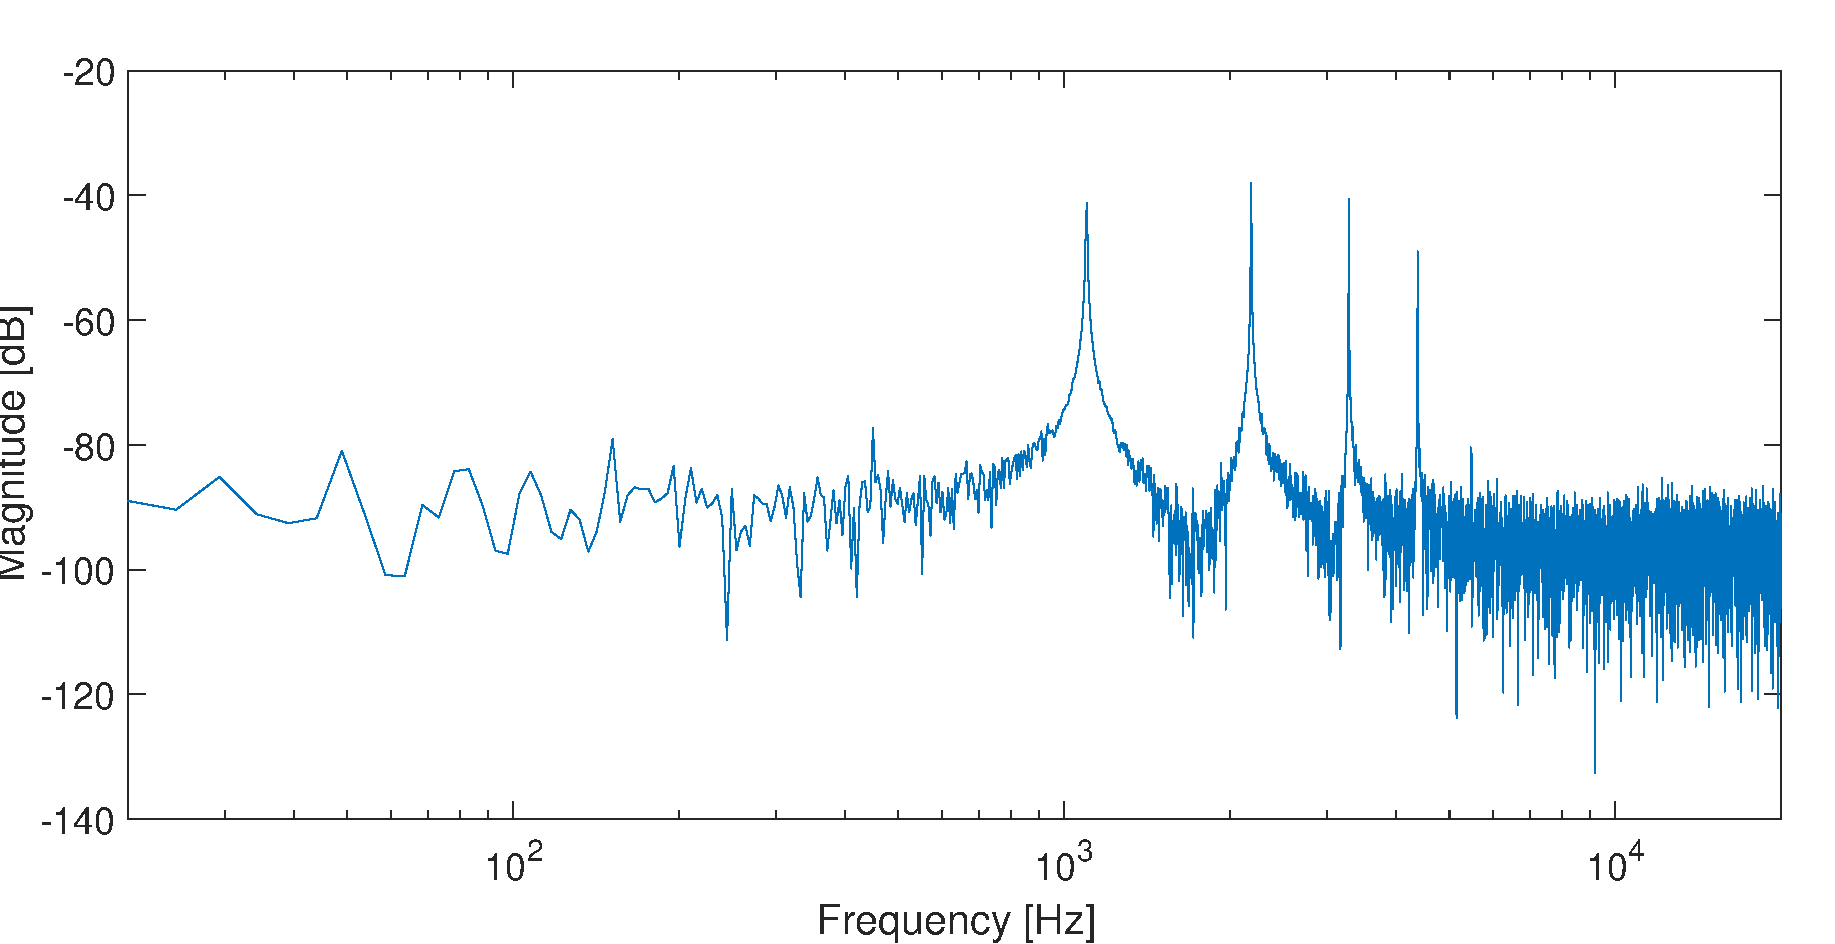
\includegraphics[width=1\textwidth]{guitar_high_Cis_bridge.pdf}
		\caption{Measurement of the high C\# note on the bridge pickup.}
		\label{fig:appendix:high_Cis_bridge}
\end{figure}

On  \autoref{fig:appendix:high_Cis_bridge} it is seen that the lowest significant frequency is around \SI{1100}{\hertz} and the highest significant frequency is around \SI{4400}{\hertz}, when playing the high C\# note on the guitar, using the bridge pickup. 

\begin{figure}[htbp!]
	\centering
		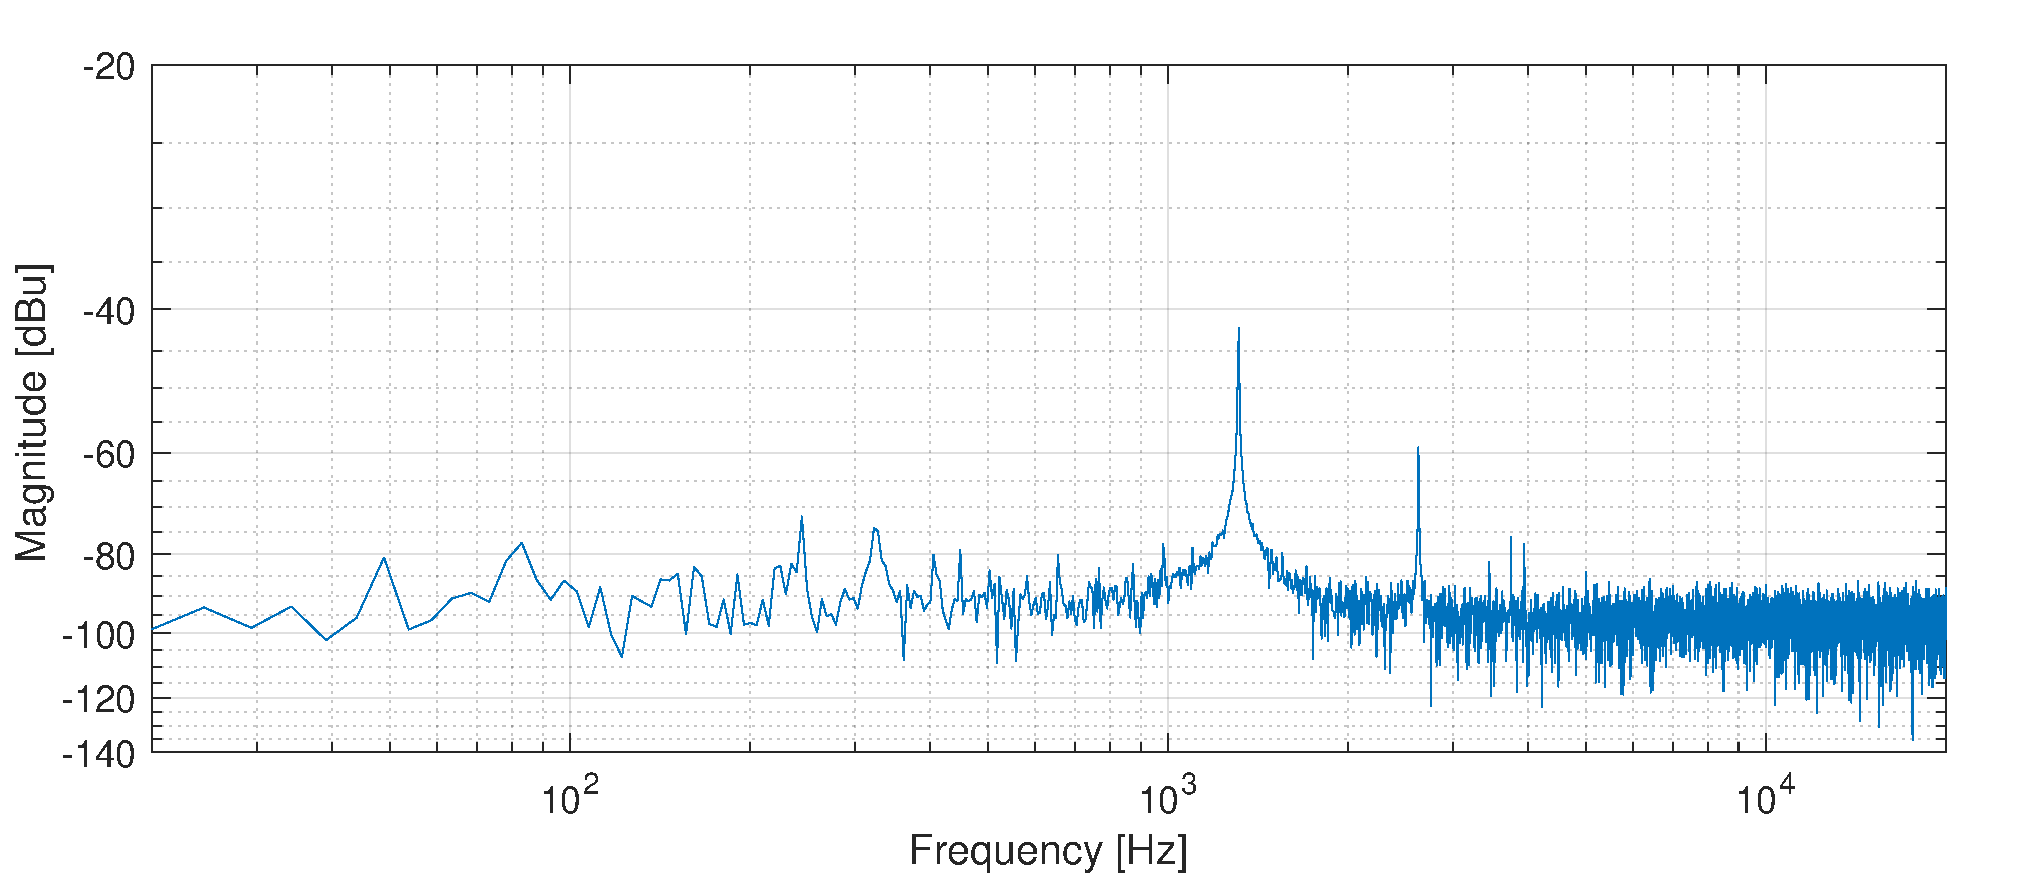
\includegraphics[width=1\textwidth]{guitar_high_E_flasholet_bridge.pdf}
		\caption{Measurement of the high E note, played as flasholet, on the bridge pickup.}
		\label{fig:appendix:high_E_bridge_flasholet}
\end{figure}

On  \autoref{fig:appendix:high_E_bridge_flasholet} it is seen that the lowest significant frequency is around \SI{1300}{\hertz} and the highest significant frequency is around \SI{2600}{\hertz}, when playing the high E note on the guitar as flasholet, using the bridge pickup. 

\chapter*{Test a guitars frequency area}
A test was made to get a view of the output impedance of a guitar.

\section*{Materials and setup}
To measure the output impedance on a guitar, the following materials are used:
\begin{itemize}
\item Digilent Analog Discovery 2 (Oscilloscope)
\item Fender Squier Classic Vibe Telecaster (Guitar)
\item Digilent Waveforms 2015 (PC - software)
\end{itemize}

\begin{figure}[htbp!]
\centering
\def\svgwidth{\columnwidth}
\chapter{Test a guitars frequency area}\label{app:frequency_area}
A test was made to get a view of the frequency area, in which the tones from a guitar lies.

\section*{Materials and setup}
To measure the frequency area on a guitar, the following materials are used:
\begin{itemize}
\item Digilent Analog Discovery 2 (Oscilloscope)
\item Fender Squier Classic Vibe Telecaster (Guitar)
\item Digilent Waveforms 2015 (PC - software)
\end{itemize}

\begin{figure}[htbp!]
\centering
\def\svgwidth{\columnwidth}
\chapter{Test a guitars frequency area}\label{app:frequency_area}
A test was made to get a view of the frequency area, in which the tones from a guitar lies.

\section*{Materials and setup}
To measure the frequency area on a guitar, the following materials are used:
\begin{itemize}
\item Digilent Analog Discovery 2 (Oscilloscope)
\item Fender Squier Classic Vibe Telecaster (Guitar)
\item Digilent Waveforms 2015 (PC - software)
\end{itemize}

\begin{figure}[htbp!]
\centering
\def\svgwidth{\columnwidth}
\input{figures/appendix/guitar_frequency_test.pdf_tex}
\caption{Setup for measuring frequency area on a guitar.}
		\label{fig:appendix:guitar_freq}
\end{figure}

\section*{Test procedure}
To the frequency area on a guitar, the following steps are made:
\begin{enumerate}
\item The materials are set up as in \autoref{fig:appendix:guitar_freq}.
\item Digilent Waveforms 2015 is set as a spectrum analyser. 
\item The guitar is set to use the neck pickup and the volume control and the tone control are turned all the way up.
\item The highest and the lowest tone on the guitar are played, measured by the oscilloscope and analysed in Digilent Waveforms 2015.
\item The guitar is set to use the bridge pickup and step 4 is repeated. 
\item The data is plotted in MATLAB.
\end{enumerate}

\section*{Results}

\begin{figure}[htbp!]
	\centering
		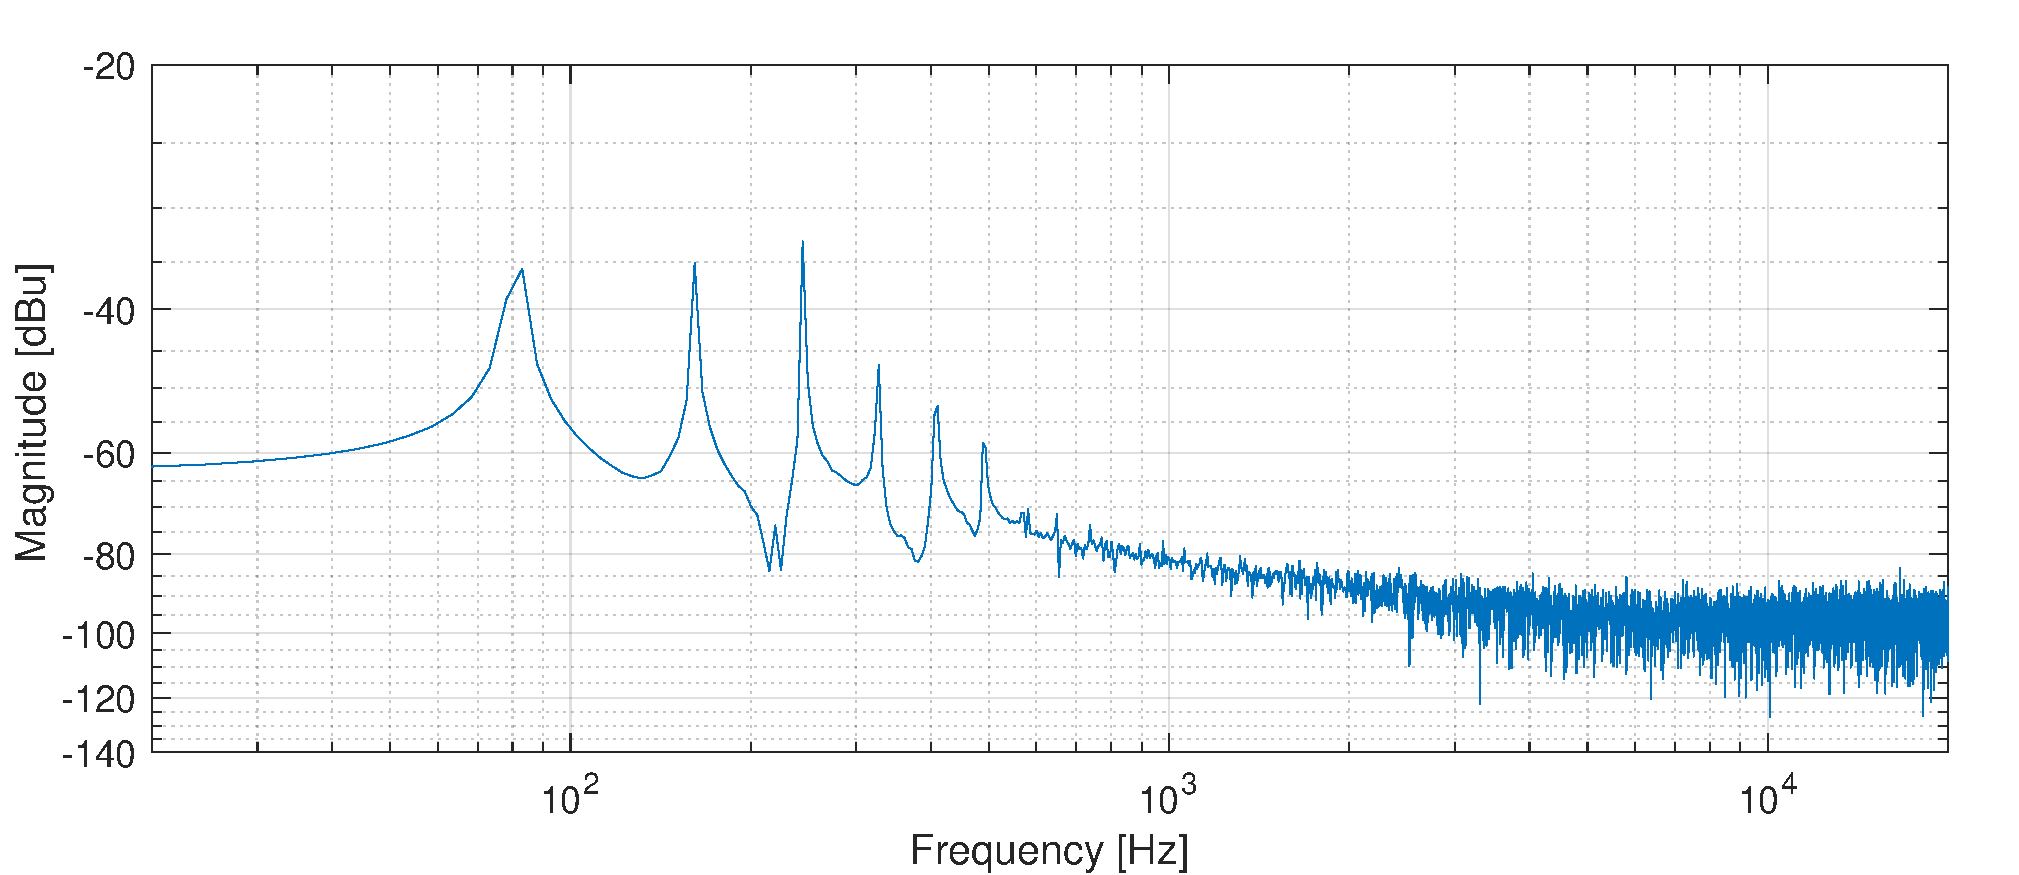
\includegraphics[width=1\textwidth]{guitar_low_E_neck.pdf}
		\caption{Measurement of the low E note on the neck pickup.}
		\label{fig:appendix:low_E_neck}
\end{figure}

On  \autoref{fig:appendix:low_E_neck} it is seen that the lowest significant frequency is around \SI{80}{\hertz} and the highest significant frequency is around \SI{400}{\hertz}, when playing the low E note on the guitar, using the neck pickup.

\begin{figure}[htbp!]
	\centering
		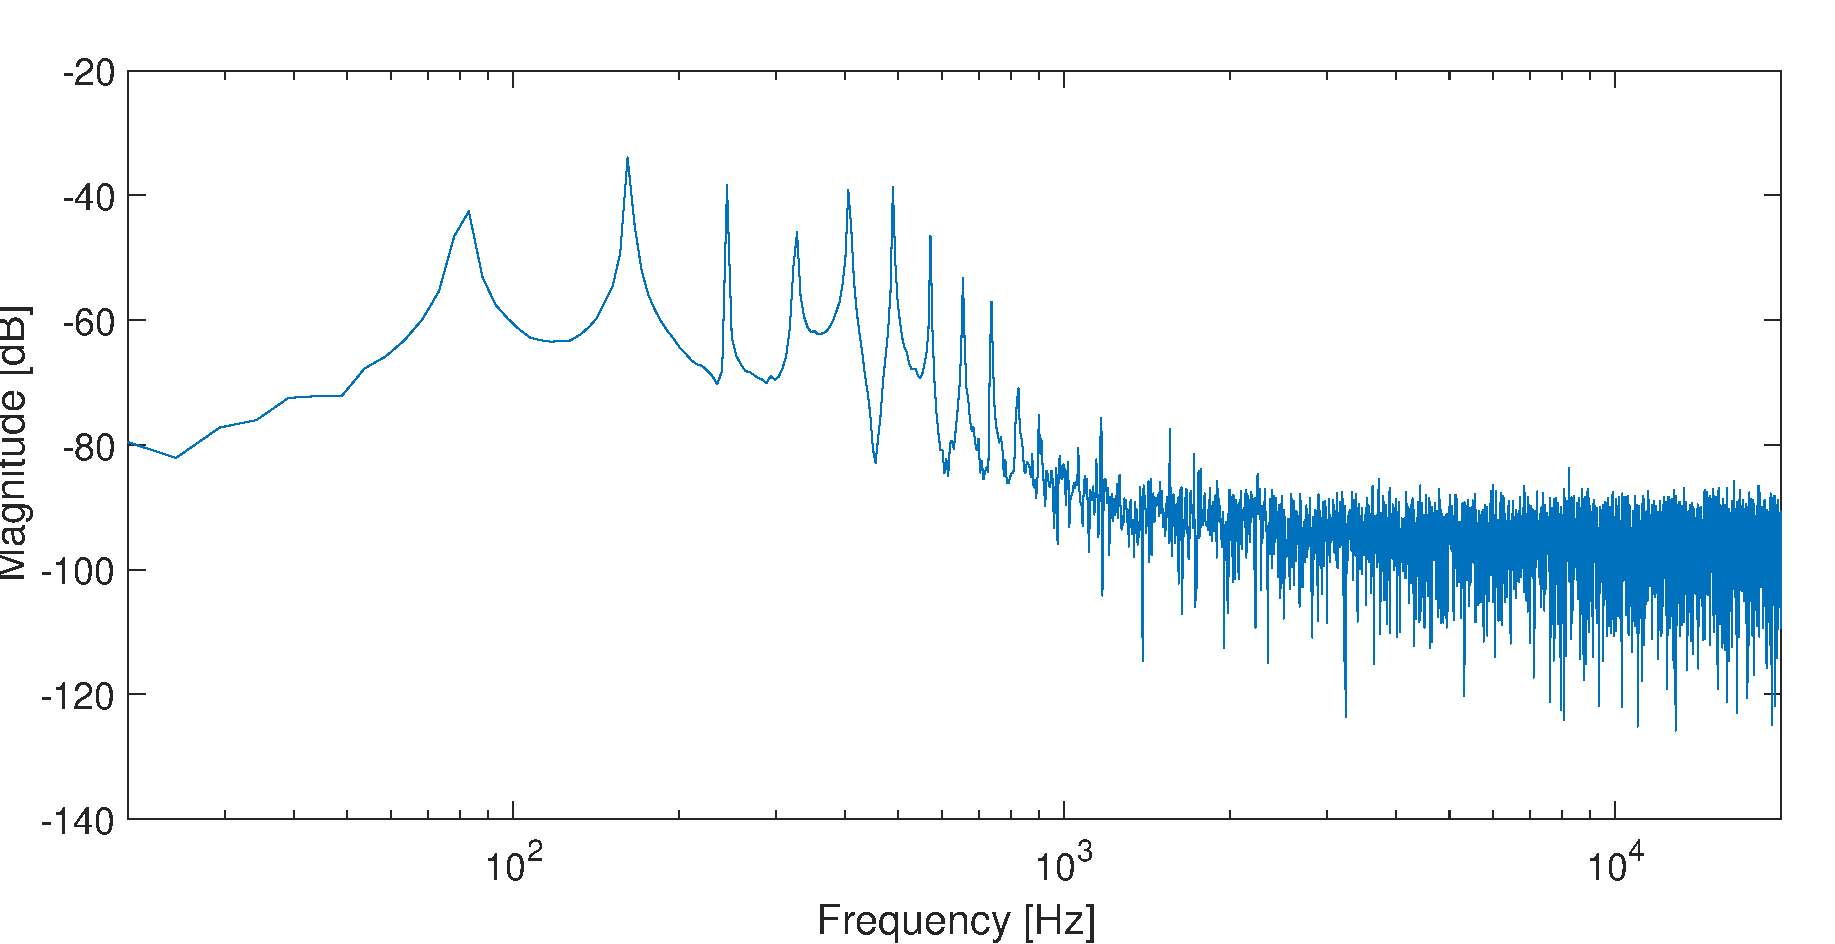
\includegraphics[width=1\textwidth]{guitar_low_E_bridge.pdf}
		\caption{Measurement of the low E note on the bridge pickup.}
		\label{fig:appendix:low_E_bridge}
\end{figure}

On  \autoref{fig:appendix:low_E_bridge} it is seen that the lowest significant frequency is around \SI{80}{\hertz} and the highest significant frequency is around \SI{730}{\hertz}, when playing the low E note on the guitar, using the bridge pickup.

\begin{figure}[htbp!]
	\centering
		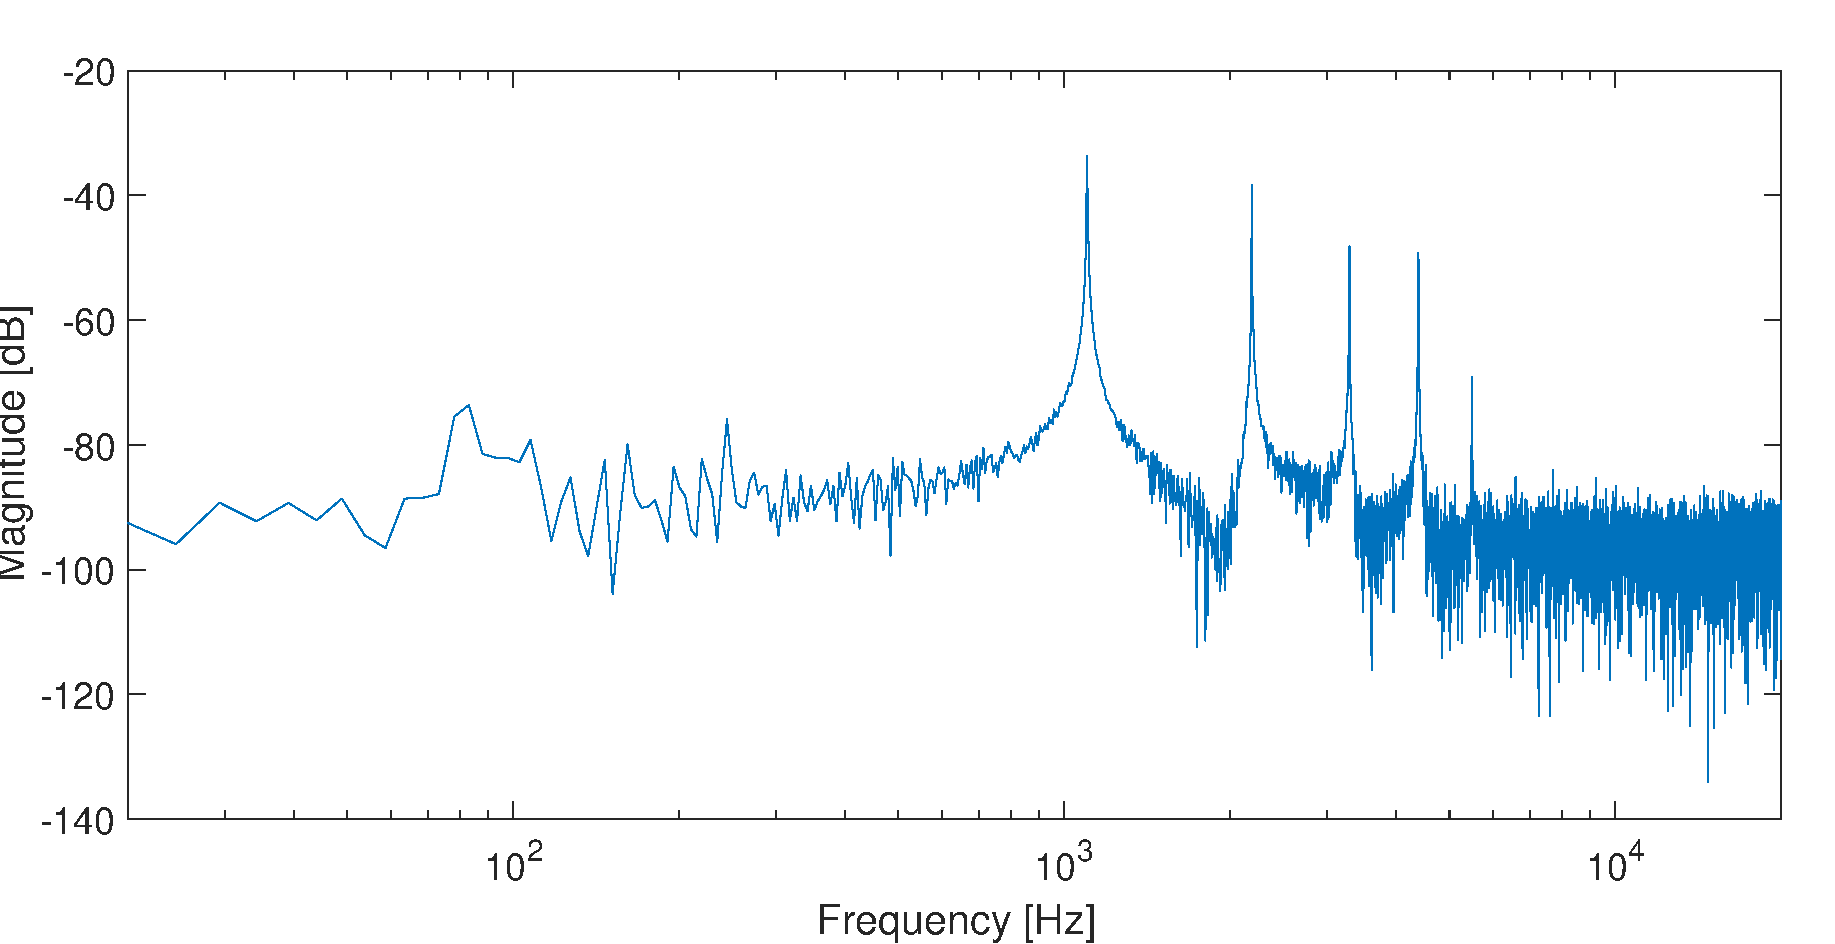
\includegraphics[width=1\textwidth]{guitar_high_Cis_neck.pdf}
		\caption{Measurement of the high C\# note on the neck pickup.}
		\label{fig:appendix:high_Cis_neck}
\end{figure}

On  \autoref{fig:appendix:high_Cis_neck} it is seen that the lowest significant frequency is around \SI{1100}{\hertz} and the highest significant frequency is around \SI{4400}{\hertz}, when playing the high C\# note on the guitar, using the neck pickup.

\begin{figure}[htbp!]
	\centering
		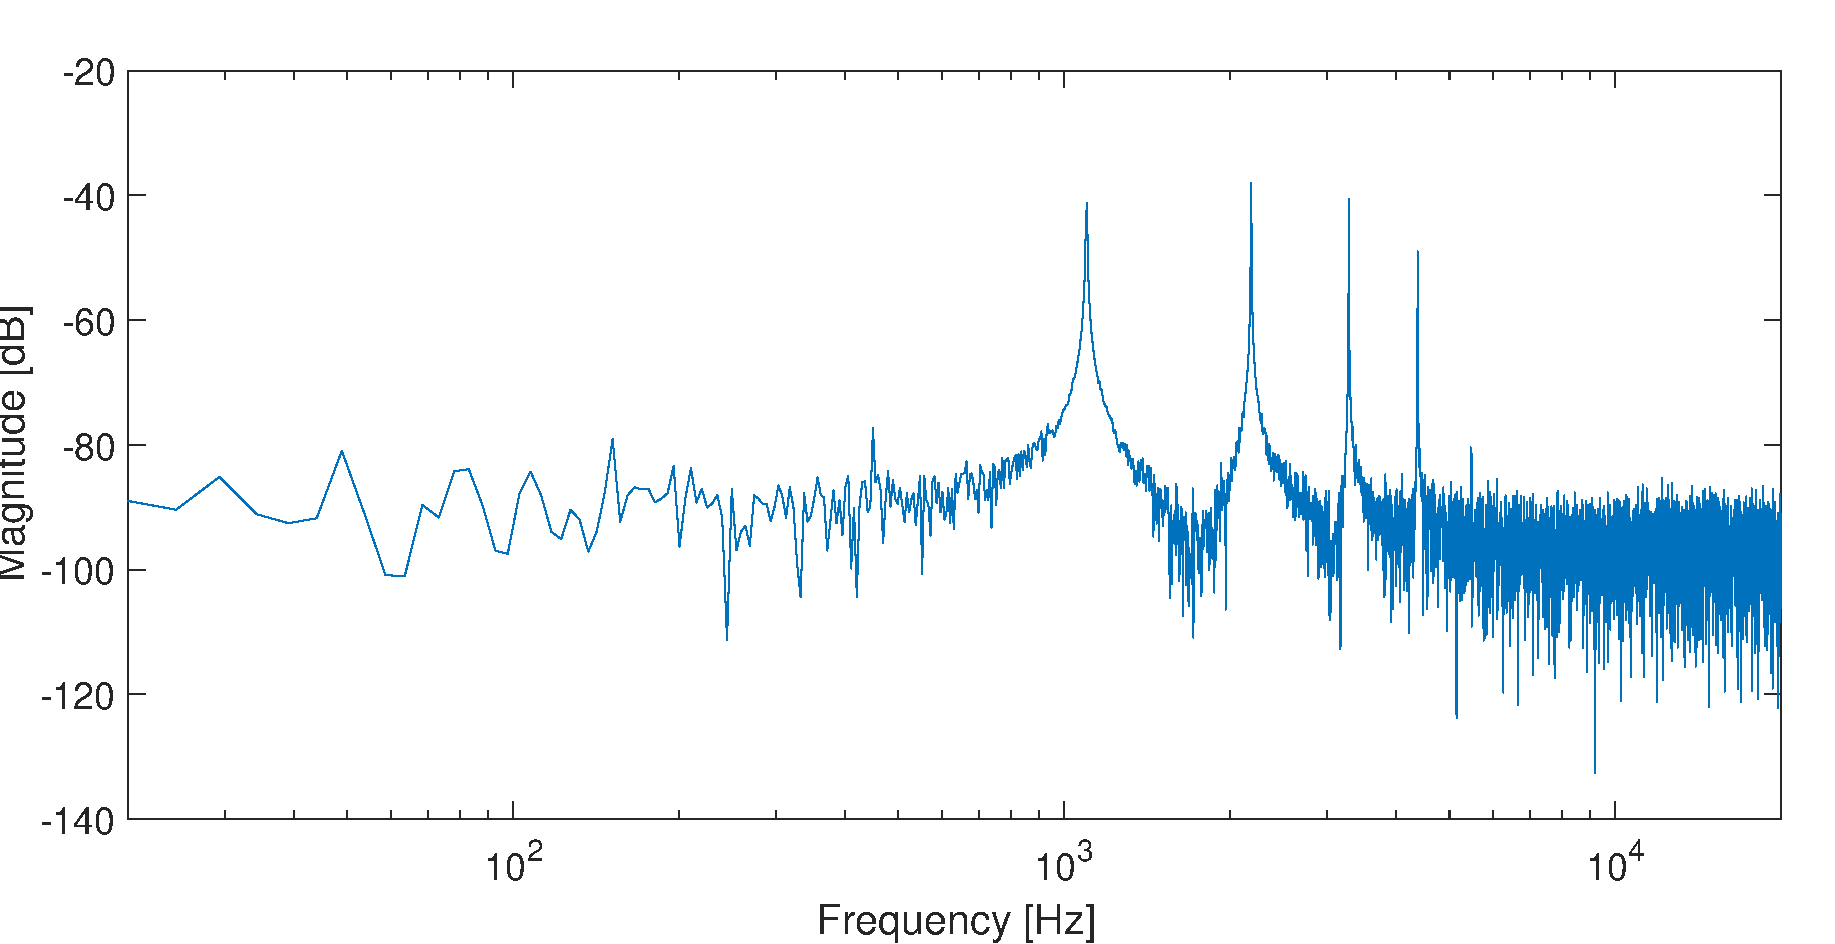
\includegraphics[width=1\textwidth]{guitar_high_Cis_bridge.pdf}
		\caption{Measurement of the high C\# note on the bridge pickup.}
		\label{fig:appendix:high_Cis_bridge}
\end{figure}

On  \autoref{fig:appendix:high_Cis_bridge} it is seen that the lowest significant frequency is around \SI{1100}{\hertz} and the highest significant frequency is around \SI{4400}{\hertz}, when playing the high C\# note on the guitar, using the bridge pickup. 

\begin{figure}[htbp!]
	\centering
		\includegraphics[width=1\textwidth]{guitar_high_E_flasholet_bridge.pdf}
		\caption{Measurement of the high E note, played as flasholet, on the bridge pickup.}
		\label{fig:appendix:high_E_bridge_flasholet}
\end{figure}

On  \autoref{fig:appendix:high_E_bridge_flasholet} it is seen that the lowest significant frequency is around \SI{1300}{\hertz} and the highest significant frequency is around \SI{2600}{\hertz}, when playing the high E note on the guitar as flasholet, using the bridge pickup. 

\caption{Setup for measuring frequency area on a guitar.}
		\label{fig:appendix:guitar_freq}
\end{figure}

\section*{Test procedure}
To the frequency area on a guitar, the following steps are made:
\begin{enumerate}
\item The materials are set up as in \autoref{fig:appendix:guitar_freq}.
\item Digilent Waveforms 2015 is set as a spectrum analyser. 
\item The guitar is set to use the neck pickup and the volume control and the tone control are turned all the way up.
\item The highest and the lowest tone on the guitar are played, measured by the oscilloscope and analysed in Digilent Waveforms 2015.
\item The guitar is set to use the bridge pickup and step 4 is repeated. 
\item The data is plotted in MATLAB.
\end{enumerate}

\section*{Results}

\begin{figure}[htbp!]
	\centering
		\includegraphics[width=1\textwidth]{guitar_low_E_neck.pdf}
		\caption{Measurement of the low E note on the neck pickup.}
		\label{fig:appendix:low_E_neck}
\end{figure}

On  \autoref{fig:appendix:low_E_neck} it is seen that the lowest significant frequency is around \SI{80}{\hertz} and the highest significant frequency is around \SI{400}{\hertz}, when playing the low E note on the guitar, using the neck pickup.

\begin{figure}[htbp!]
	\centering
		\includegraphics[width=1\textwidth]{guitar_low_E_bridge.pdf}
		\caption{Measurement of the low E note on the bridge pickup.}
		\label{fig:appendix:low_E_bridge}
\end{figure}

On  \autoref{fig:appendix:low_E_bridge} it is seen that the lowest significant frequency is around \SI{80}{\hertz} and the highest significant frequency is around \SI{730}{\hertz}, when playing the low E note on the guitar, using the bridge pickup.

\begin{figure}[htbp!]
	\centering
		\includegraphics[width=1\textwidth]{guitar_high_Cis_neck.pdf}
		\caption{Measurement of the high C\# note on the neck pickup.}
		\label{fig:appendix:high_Cis_neck}
\end{figure}

On  \autoref{fig:appendix:high_Cis_neck} it is seen that the lowest significant frequency is around \SI{1100}{\hertz} and the highest significant frequency is around \SI{4400}{\hertz}, when playing the high C\# note on the guitar, using the neck pickup.

\begin{figure}[htbp!]
	\centering
		\includegraphics[width=1\textwidth]{guitar_high_Cis_bridge.pdf}
		\caption{Measurement of the high C\# note on the bridge pickup.}
		\label{fig:appendix:high_Cis_bridge}
\end{figure}

On  \autoref{fig:appendix:high_Cis_bridge} it is seen that the lowest significant frequency is around \SI{1100}{\hertz} and the highest significant frequency is around \SI{4400}{\hertz}, when playing the high C\# note on the guitar, using the bridge pickup. 

\begin{figure}[htbp!]
	\centering
		\includegraphics[width=1\textwidth]{guitar_high_E_flasholet_bridge.pdf}
		\caption{Measurement of the high E note, played as flasholet, on the bridge pickup.}
		\label{fig:appendix:high_E_bridge_flasholet}
\end{figure}

On  \autoref{fig:appendix:high_E_bridge_flasholet} it is seen that the lowest significant frequency is around \SI{1300}{\hertz} and the highest significant frequency is around \SI{2600}{\hertz}, when playing the high E note on the guitar as flasholet, using the bridge pickup. 

\caption{Setup for measuring frequency area on a guitar.}
		\label{fig:appendix:guitar_freq}
\end{figure}

\section*{Test procedure}


\begin{enumerate}
\item The materials are set up as in \autoref{fig:appendix:guitar_output_impedance}.
\item 
\item  
\item  
\item 
\item 
\end{enumerate}

\section*{Results}

\begin{figure}[htbp!]
	\centering
		\includegraphics[width=1\textwidth]{guitar_low_E_neck.pdf}
		\caption{Measurement of the low E note on the neck pickup.}
		\label{fig:appendix:low_E_neck}
\end{figure}

On  \autoref{fig:appendix:low_E_neck} it is seen that the lowest significant frequency is around \SI{80}{\hertz} and the highest significant frequency is around \SI{400}{\hertz}, when playing the low E note on the guitar, using the neck pickup.


